% Body of the final report (abstract to appendices), for COMPSCI 4411/9538, Group 6.
%
% To use it in the course Overleaf template (copy the template first, it is read-only):
%   1. Upload this file, references.bib and the figures/ folder to the project.
%   2. In the template's main file, after the title block, add:  % Body of the final report (abstract to appendices), for COMPSCI 4411/9538, Group 6.
%
% To use it in the course Overleaf template (copy the template first, it is read-only):
%   1. Upload this file, references.bib and the figures/ folder to the project.
%   2. In the template's main file, after the title block, add:  % Body of the final report (abstract to appendices), for COMPSCI 4411/9538, Group 6.
%
% To use it in the course Overleaf template (copy the template first, it is read-only):
%   1. Upload this file, references.bib and the figures/ folder to the project.
%   2. In the template's main file, after the title block, add:  % Body of the final report (abstract to appendices), for COMPSCI 4411/9538, Group 6.
%
% To use it in the course Overleaf template (copy the template first, it is read-only):
%   1. Upload this file, references.bib and the figures/ folder to the project.
%   2. In the template's main file, after the title block, add:  \input{body}
%   3. Add the packages below to the template's preamble if it does not load them already:
%        booktabs, tabularx, array, graphicx, float, caption, enumitem, tikz (with libraries
%        positioning, arrows.meta, shapes.geometric, fit, backgrounds), xurl, hyperref
%        and this macro:   \newcommand{\code}[1]{\texttt{#1}}
%        and this column type:   \newcolumntype{Y}{>{\raggedright\arraybackslash}X}
%        and:   \graphicspath{{figures/}}
%   4. If the template sets up its own bibliography, delete the two lines near the end of this file
%      (\bibliographystyle and \bibliography) and keep the template's.
%
% report/main.tex is a ready-made wrapper that does exactly this, so it compiles on its own.

\begin{abstract}
Trading desks want per-minute summaries and alerts within seconds of each trade. We built that
pipeline from Apache Kafka 4.4 (three brokers, KRaft) and Spark 4.2 Structured Streaming (PySpark).
It writes one-minute open, high, low, close and volume-weighted average price (VWAP) bars and
three-sigma alerts to PostgreSQL, shows them in Grafana, and starts with one \code{docker compose up}.
A seeded generator makes the correct output known exactly, so we check every run bar by bar. We
reproduce two published results, producer batching (Kreps et al., Figure 4) and continuous versus
micro-batch latency (Armbrust et al., Figure 7), and add what neither paper measured: whether the output
stays correct when a broker or the Spark job crashes, and what exactly-once output costs. No
acknowledged trade was lost in 12 broker crashes. Spark recovered from its own crash in about 14
seconds with exact output. Plain inserts left 300 duplicate rows after every crash, while upserts left
none and cost nothing we could measure at 2,000 trades per second. All measurements come from one
4-CPU machine, and Section~\ref{sec:limits} says what that does to the conclusions.
\end{abstract}

%------------------------------------------------------------------------------------------------
\section{Background and significance}
Market data arrives as a continuous stream of trades. A common design pairs a durable, partitioned
log that stores the events with a stream processor that reads the log and computes results over time
windows.

\paragraph{Apache Kafka.} Kafka~\cite{kreps2011,wang2015} is the log. A topic is split into
partitions, and each partition is an append-only file on a broker, written and read sequentially in
batches. Kreps et al.\ showed that this gives much higher throughput than traditional message
queues~\cite{kreps2011}. Kafka orders events only within a partition, so keying trades by symbol keeps
each symbol's trades in order. Each partition is copied to several brokers: a leader serves reads and
writes, and the followers that are caught up form the in-sync replica set (ISR). Whether an acknowledged
write survives a broker crash depends on three settings: the replication factor, the number of copies
the producer waits for (\code{acks}), and the minimum number of in-sync replicas~\cite{wang2015}. Kafka 4
keeps cluster metadata in its own Raft-based protocol (KRaft), so it no longer needs ZooKeeper.

\paragraph{Spark Structured Streaming.} Structured Streaming~\cite{armbrust2018} is the processor. It
treats a stream as an unbounded table and runs a normal SQL-style query over it incrementally, usually
in micro-batches, an approach that descends from discretized streams~\cite{zaharia2013}. It aggregates
over event-time windows and keeps intermediate state between batches. A watermark says how long Spark
waits for late events before it finalizes a window, an idea from the Dataflow model~\cite{akidau2015}.
Spark records each batch's Kafka offsets and its state in a checkpoint. Kafka can re-deliver from any
offset, so after a crash Spark re-runs exactly the unfinished batches, and an idempotent sink then makes
the result the same as if each event had been processed once. An experimental continuous mode lowers
latency, but it supports only per-record operations and delivers at least once.

\paragraph{Why test them together.} The papers promise high throughput from batched sequential I/O,
durability from replication, and exactly-once results from replay plus checkpoints. Each promise
depends on configuration and on how the two systems are connected. We test them on a financial
workload with a known correct answer, and we focus on the seam between the systems more than on either
one alone.

%------------------------------------------------------------------------------------------------
\section{Goals and objectives}
We set out to answer three research questions.
\begin{enumerate}[label=\textbf{RQ\arabic*.},leftmargin=*]
  \item How do the number of partitions, the trigger interval and the processing mode trade latency
        against throughput?
  \item Which Kafka settings prevent lost or duplicated data when a broker crashes, and how long does
        Spark take to recover from its own crash?
  \item What does exactly-once output cost compared with at-least-once output?
\end{enumerate}
The objectives are: (1) explain how Kafka, Spark and their integration work; (2) build a case-study
pipeline that starts with one command; (3) reproduce Kreps et al.\ Figure~4 and Armbrust et al.\
Figure~7, comparing the shape of each curve and not the absolute numbers; (4) extend both papers with
experiments they did not run, namely correctness under crashes and the cost of exactly-once output;
and (5) publish a repository that others can run, with pinned versions and scripted experiments.

%------------------------------------------------------------------------------------------------
\section{Architecture analysis}
\label{sec:arch}
Figure~\ref{fig:pipeline} shows the pipeline we built. A generator publishes trades, keyed by symbol,
to a topic with six partitions. Spark reads one task per partition, builds one-minute bars with a
10-second watermark, and writes each batch to PostgreSQL in one transaction. Grafana reads PostgreSQL.

\begin{figure}[H]
\centering
\resizebox{\textwidth}{!}{%
\begin{tikzpicture}[
  node distance=9mm and 8mm,
  box/.style={draw,rounded corners=2pt,align=center,inner sep=4pt,font=\small,minimum height=10mm},
  store/.style={draw,cylinder,shape border rotate=90,aspect=0.25,align=center,font=\small,minimum height=11mm,inner sep=3pt},
  arr/.style={-{Stealth[length=2mm]},thick},
  lab/.style={font=\scriptsize,align=center}]
  \node[box] (gen) {Generator\\(seeded, or\\Coinbase live)};
  \node[box,right=26mm of gen] (kafka) {Kafka, 3 brokers\\topic \code{trades}\\6 partitions, RF 3,\\min ISR 2};
  \node[box,right=26mm of kafka] (spark) {Spark\\\code{local[4]}, 1 s trigger\\watermark 10 s,\\1-minute windows};
  \node[store,right=30mm of spark] (pg) {PostgreSQL\\bars, alerts};
  \node[box,right=12mm of pg] (graf) {Grafana};
  \node[store,below=8mm of spark] (ck) {Checkpoint\\volume};
  \draw[arr] (gen) -- node[lab,above]{key = symbol} node[lab,below]{acks=all} (kafka);
  \draw[arr] (kafka) -- node[lab,above]{one task per} node[lab,below]{partition} (spark);
  \draw[arr] (spark) -- node[lab,above]{one transaction} node[lab,below]{per batch} (pg);
  \draw[arr] (pg) -- (graf);
  \draw[arr,dashed] (spark) -- node[lab,right]{offsets, state} (ck);
\end{tikzpicture}}
\caption{The pipeline. A separate pass-through job (not shown) copies \code{trades} to a second
topic for the latency experiments.}
\label{fig:pipeline}
\end{figure}

\subsection{Kafka}
Table~\ref{tab:kafka} lists the Kafka mechanisms we rely on and where each one shows up in the project.

\begin{table}[H]
\centering\small
\caption{Kafka mechanisms and their role in this project.}
\label{tab:kafka}
\begin{tabularx}{\textwidth}{@{}>{\raggedright\arraybackslash}p{3.1cm}YY@{}}
\toprule
Mechanism & How it works & In this project \\
\midrule
Partitions and ordering & A partition is an append-only log on a broker, written and read sequentially. Order holds only within a partition; the producer picks the partition by hashing the key. & \code{trades} has 6 partitions on 3 brokers. Key = symbol, so every symbol lands in one partition and stays in order (checked from the acknowledgement log). \\
Throughput design~\cite{kreps2011} & Batching many records per request, sequential disk I/O, the page cache, zero-copy transfer. & E1a reproduces the batching effect. \\
Retention & Records stay for a time or size limit whether or not they were read, so a consumer can re-read from any offset. & \code{trades} keeps one day. Replay after a crash depends on it. \\
Replication and ISR~\cite{wang2015} & A partition has a leader and followers. A write is committed when every in-sync replica has it. & RF 3, \code{min.insync.replicas=2}, unclean leader election off, so only an in-sync replica can become leader. \\
Producer \code{acks} & 0: no wait. 1: the leader only. all: every in-sync replica. & E2 kills a leader with acks=1 and acks=all. \\
Idempotent producer & The broker drops a retried batch it has already seen, using the producer id and a sequence number. & On by default with acks=all. Without it, a leader kill once duplicated a trade (Section~\ref{sec:challenges}). \\
KRaft & Metadata lives in a Raft-replicated log on controller nodes. & Three nodes, each broker and controller. \\
Consumer groups & Consumers with one \code{group.id} split a topic's partitions, and Kafka stores the group's committed offsets. & Used by our verifier and latency collectors. Spark does not use them (Section~\ref{sec:integration}). \\
Delivery guarantees & At most once, at least once, or exactly once (idempotent producer plus transactions inside Kafka). & End-to-end exactly-once here comes from Spark's replay plus an idempotent sink. \\
Security & TLS encrypts traffic, SASL authenticates clients, ACLs authorize operations. & Described, not measured. The stack runs PLAINTEXT on one machine, with Grafana and PostgreSQL bound to localhost. \\
\bottomrule
\end{tabularx}
\end{table}

\subsection{Spark Structured Streaming}
Table~\ref{tab:spark} does the same for Spark.

\begin{table}[H]
\centering\small
\caption{Spark mechanisms and their role in this project.}
\label{tab:spark}
\begin{tabularx}{\textwidth}{@{}>{\raggedright\arraybackslash}p{3.1cm}YY@{}}
\toprule
Mechanism & How it works & In this project \\
\midrule
Unbounded table~\cite{armbrust2018} & A streaming query is an ordinary DataFrame query that Spark runs incrementally. The optimizer turns it into an incremental plan with stateful operators. & The bars job is a \code{groupBy(window, symbol)} aggregation. \\
Micro-batch and triggers~\cite{zaharia2013} & A trigger starts a batch at fixed intervals; each batch reads the offsets that arrived since the last one. & Trigger 1 s by default. E1c varies it from 100 ms to 5 s. \\
Continuous processing & Long-running tasks handle one record at a time and checkpoint in epochs. Lower latency, but only map-like operations, at-least-once, and one core per input partition. & Cannot run the bars job. E1b runs a pass-through job in both modes. With 6 partitions on 4 cores, two partitions were never processed. \\
Event time and watermark~\cite{akidau2015} & Windows follow the record's event time. The watermark is the largest event time seen minus a delay. In append mode a window is emitted once, when the watermark passes its end. & One-minute tumbling windows, 10 s watermark. A closing trade for a reserved symbol advances the watermark past the last windows. \\
State store & Partial aggregates per window and key, written to the checkpoint every batch and dropped after the watermark passes. & Open, high, low, close (using \code{min\_by} and \code{max\_by} on time and trade id), volume, notional, count. \\
Checkpoint & \code{offsets/} (the range each batch will read, written before processing), \code{commits/} (finished batches), \code{state/}. & A named volume that survives \code{docker kill}. E3 and E4 depend on it. \\
Sinks & Append, update or complete output; \code{foreachBatch} hands each batch to user code; the Kafka sink is at least once. & Append mode with \code{foreachBatch} into PostgreSQL. The pass-through job uses the Kafka sink. \\
Monitoring & A \code{StreamingQueryListener} receives one progress event per batch. & Written to a \code{query\_progress} table that feeds the dashboard and the throughput tests. \\
\bottomrule
\end{tabularx}
\end{table}

\subsection{Integration}
\label{sec:integration}
\paragraph{Partitions become tasks.} The Kafka source plans one Spark task per Kafka partition in each
batch, so the partition count bounds parallelism. E1c compares 1, 3 and 6 partitions on 4 cores.

\paragraph{Offsets live in Spark's checkpoint, not in a consumer group.} Spark picks each batch's offset
range and writes it to the checkpoint before it processes anything. That ties the offsets to the batch
id and to a version of the state. A consumer group's committed offset cannot do that: it says
``consumed'', not ``consumed and reflected in state version $n$ and in output batch $n$''. After a
crash Spark reads exactly the uncommitted range again. This requires Kafka to still hold the data
(\code{failOnDataLoss=true} stops the query if it does not) and the checkpoint to match the topic, so our
harness always wipes both together.

\paragraph{Exactly-once output is replay plus an idempotent sink.} Replay delivers a crashed batch a
second time, and the sink must make the second write harmless. Each batch's bars and alerts go to
PostgreSQL in one transaction, using \code{INSERT ... ON CONFLICT (symbol, window\_start) DO UPDATE},
and the \code{written\_at} column is set only on the first insert. Figure~\ref{fig:batch} shows the order
of events in one batch. A crash anywhere before the commit record makes Spark run the batch again from
the same offsets, and the upsert absorbs it. E4 tests exactly that.

\begin{figure}[H]
\centering\small
\begin{tabularx}{\textwidth}{@{}rlY@{}}
\toprule
Step & Actor & Action \\
\midrule
1 & Spark driver & Ask Kafka for the latest offset of every partition. \\
2 & Spark driver & Write the planned offset range to the checkpoint (\code{offsets/n}). \\
3 & Spark tasks & Read that range, one task per partition, and update the aggregation state. \\
4 & Spark driver & Emit the windows the watermark has passed. \\
5 & Sink & In one transaction: upsert the bars, read the 31 previous bars of each symbol, upsert the alerts, commit. \\
6 & Spark driver & Write \code{commits/n} and state version $n$. \\
\bottomrule
\end{tabularx}
\caption{One micro-batch. A crash between steps 5 and 6 replays the batch.}
\label{fig:batch}
\end{figure}

\subsection{Failure behavior}
Table~\ref{tab:failure} lists each failure we injected or considered and what the experiments showed.

\begin{table}[H]
\centering\small
\caption{Failure behavior and where we measured it.}
\label{tab:failure}
\begin{tabularx}{\textwidth}{@{}>{\raggedright\arraybackslash}p{3.6cm}Yl@{}}
\toprule
Failure & What happens & Measured in \\
\midrule
Leader broker killed, acks=all & Writes to every partition stall until the controller fences the dead broker and removes it from the ISR; then they continue. No acknowledged trade is lost. The stall matches \code{broker.session.timeout.ms} (9,000 ms) plus up to one heartbeat interval. & E2 \\
Leader broker killed, acks=1 & Only the partitions the dead broker led stall. Records it had acknowledged but not yet replicated can be lost when a follower takes over; not every kill loses data. & E2 \\
Producer retry without idempotence & A retried batch can be written twice. & E2, Section~\ref{sec:challenges} \\
Spark killed & Spark restarts from the checkpoint. Recovery time is mostly JVM and Spark start-up. Output stays exact with the upsert sink. & E3 \\
Spark killed after the sink commits & Spark replays the batch: duplicates with plain inserts, none with upserts. & E4 \\
Topic recreated under a checkpoint & \code{failOnDataLoss=true} stops the query instead of skipping data. & Harness procedure \\
\bottomrule
\end{tabularx}
\end{table}

\subsection{Design choices}
Several choices trade one property for another. A shorter watermark lowers bar latency but drops more
late trades, and because we measure latency from the window end plus the watermark, the watermark
adds directly to the time to result. A shorter trigger lowers latency but adds per-batch overhead
(E1c). More partitions add parallel tasks but also state-store and planning work on four cores. Setting
acks=all with a minimum ISR of 2 survives one broker failure at the price of a write stall while the
ISR shrinks (E2). We read the alert history back from PostgreSQL, which keeps the Spark job a plain
windowed aggregation, at the cost of one indexed query per batch. Running Spark as \code{local[4]} in one
container matches the 4-core setup of Armbrust et al.\ and our memory budget, but it is not a test of
distributed Spark.

%------------------------------------------------------------------------------------------------
\section{Features exercised}
\begin{table}[H]
\centering\small
\caption{Each feature, how the pipeline uses it, and what demonstrates it.}
\begin{tabularx}{\textwidth}{@{}>{\raggedright\arraybackslash}p{3.4cm}YY@{}}
\toprule
Feature & Use in the pipeline & Demonstrated by \\
\midrule
Partitioned, keyed log & 6 partitions, key = symbol, per-symbol order & Acknowledgement-log check; E1c \\
Replication and acks & RF 3, min ISR 2, acks=all, idempotent producer & E2 \\
Event-time windows and watermark & 1-minute bars, 10 s watermark, append mode & 4,000 bars match the oracle exactly \\
Stateful lookback & Alert when the log return is more than 3 standard deviations from the previous 30 bars & 23 of 23 expected alerts; 20 of 20 injected shocks found \\
Checkpoint recovery & Restart from offsets and state after SIGKILL & E3 \\
Exactly-once output & One transaction per batch, upsert on (symbol, minute) & E4 \\
Continuous processing & Kafka-to-Kafka pass-through & E1b \\
Monitoring & Progress listener to \code{query\_progress}, Grafana dashboard & Live dashboard \\
\bottomrule
\end{tabularx}
\end{table}

%------------------------------------------------------------------------------------------------
\section{Case study: the market-data pipeline}
\paragraph{Generator.} A seeded generator makes random-walk prices for 100 symbols. The busiest symbol
trades about ten times as often as the quietest, sizes are log-normal, and permanent price shocks of
1.5\% to 3\% happen at known times after a 30-bar warm-up, so we know which alerts must fire. It has
virtual, realtime and replay modes and writes a per-trade acknowledgement log. A fourth mode reads live
trades from Coinbase, with capture and replay as a fallback.

\paragraph{Spark job.} The job parses the JSON with an explicit schema and groups by symbol and
one-minute window. Open and close come from \code{min\_by} and \code{max\_by} ordered by event time and
trade id, so they do not depend on arrival order. VWAP uses \code{try\_divide} because Spark 4 raises an
error on division by zero.

\paragraph{Alert rule.} Our proposal says an alert fires when a price change is more than three
standard deviations from that symbol's average over the previous 30 bars. We read ``price change'' as
the bar-to-bar log return of the close. For each bar we take the 30 previous returns, compute their
mean and sample standard deviation, and alert when the new return differs from the mean by more than
three standard deviations. A symbol with fewer than 31 bars, or with zero variance, never alerts.

\paragraph{Sink and dashboard.} Each batch is one PostgreSQL transaction (Section~\ref{sec:integration}).
Grafana shows candlesticks, VWAP, alerts and Spark's own progress metrics.

\paragraph{Verification.} We treat verification as part of the system. An oracle
(\path{tools/gen_sample_dataset.py}, copied into \path{verify/reference.py}) computes the exact expected bars
and alerts. The verifier compares every bar (open, high, low and close exactly, VWAP within $10^{-6}$)
and every alert, and a second verifier compares the producer's acknowledgement log with the contents of
the topic. A run therefore passes or fails, including every crash experiment. The golden dataset has
60,163 trades, 4,000 bars, 23 alerts and 20 shocks, and its SHA-256 hashes are in a manifest.

%------------------------------------------------------------------------------------------------
\section{Experiments and results}
\label{sec:results}
\paragraph{Setup.} All experiments ran on one virtual machine with 4 CPUs, 16 GB of memory and Docker,
alone on it, three runs per setting (six kills for E2 with acks=1). Latency is the median over runs of
each run's p50, p95 and p99. Sustained throughput is the highest input rate at which Spark keeps up
over a five-minute run. We drop a warm-up period from every latency measurement, because JVM
start-up made the first seconds about twenty times slower. Ranges in brackets are the minimum and
maximum over runs. The machine and versions are in Appendix~\ref{app:machine}, and the Kafka, Spark
and producer settings of every experiment are in Appendix~\ref{app:config}.

\subsection{E1a: producer batching (reproduction of Kreps et al., Figure 4)}
We ran Kafka's own producer performance tool with acks=0, 10 million records of 200 bytes, and one
partition with no replication, as the paper did, varying the batch size.

\begin{table}[H]
\centering\small
\caption{E1a: producer throughput against batch size (median of 3 runs).}
\label{tab:e1a}
\begin{tabular}{@{}lrrrrr@{}}
\toprule
Batch size (messages) & 1 & 10 & 50 & 100 & 200 \\
\midrule
Records per second & 19,798 & 154,909 & 525,376 & 739,153 & 848,033 \\
\bottomrule
\end{tabular}
\end{table}

Batching raised throughput 26 times from 1 to 50 messages per batch. The paper reports about 8 times,
from roughly 50,000 to 400,000 messages per second. With acks=0 the tool's latency column means
nothing, so we do not report it. See Figure~\ref{fig:e1a}.

\begin{figure}[H]
\centering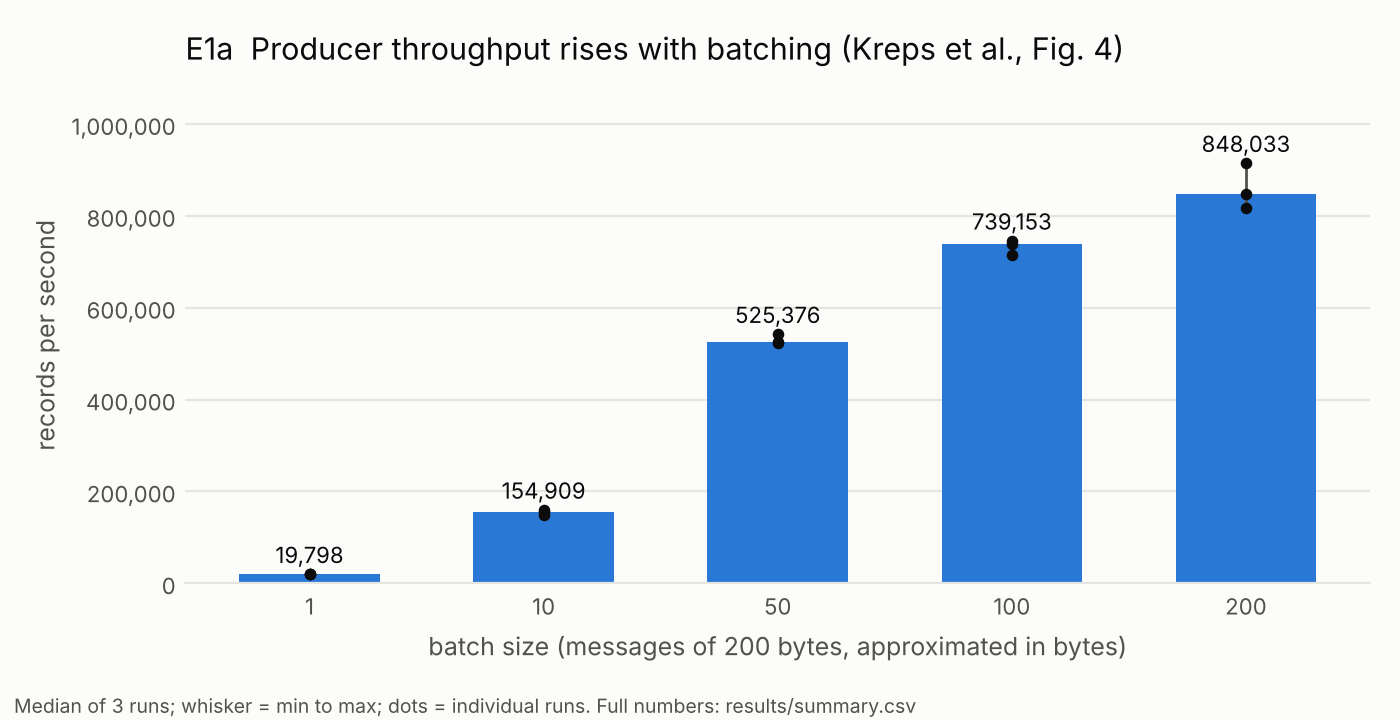
\includegraphics[width=0.8\textwidth]{e1a_producer_batching.png}
\caption{E1a: batching raises producer throughput.}
\label{fig:e1a}
\end{figure}

\subsection{E1b: continuous versus micro-batch (reproduction of Armbrust et al., Figure 7)}
A stateless pass-through job copies one topic to another. In continuous mode with 4 partitions, median
latency was 43 to 83 ms from 5,000 to 40,000 records per second (p99 0.3 to 0.9 s). At 80,000 records per
second its four tasks saturated: p50 rose to 1.8 s and p99 to 6.9 s. Micro-batch mode with a 100 ms
trigger kept up with the highest rate we could generate, at least 100,000 records per second, with
p50 between 0.27 and 0.62 s. See Figure~\ref{fig:e1b}.

\begin{figure}[H]
\centering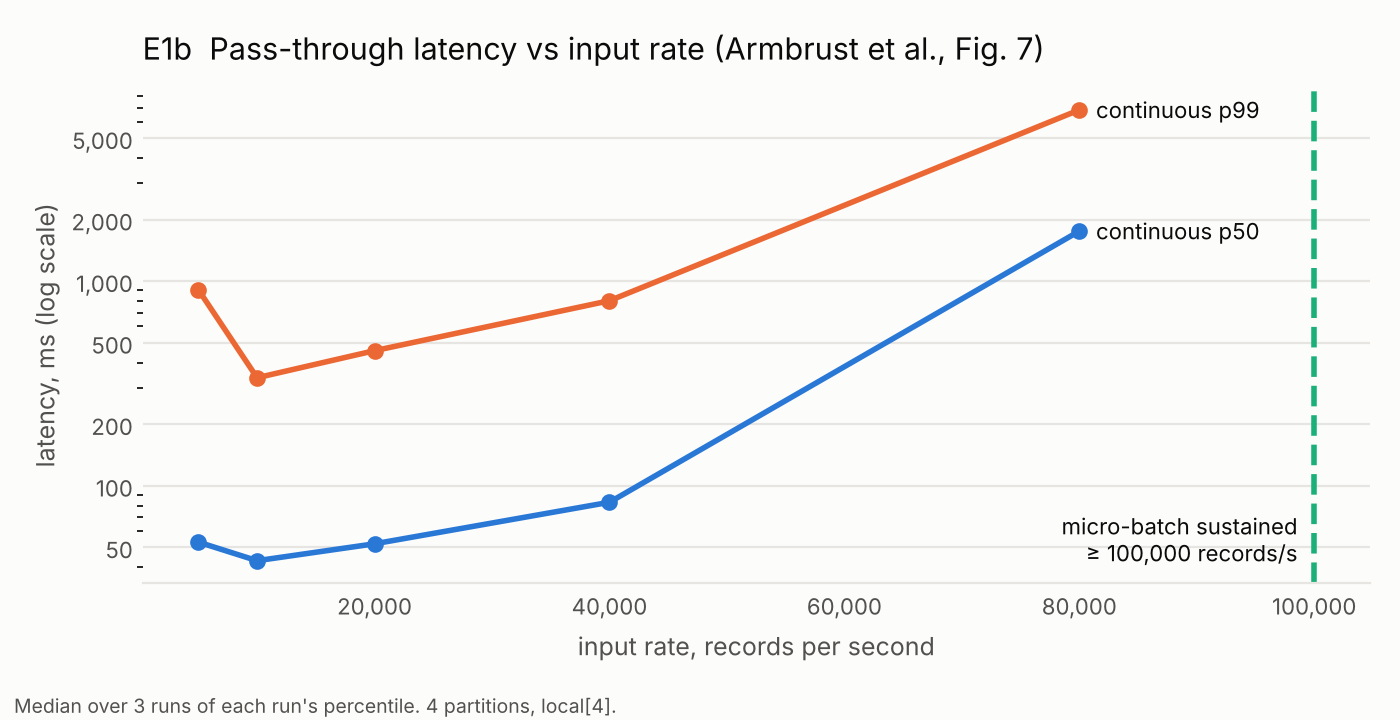
\includegraphics[width=0.85\textwidth]{e1b_continuous_vs_microbatch.png}
\caption{E1b: continuous mode has the lower latency until it saturates; micro-batch sustains a higher rate.}
\label{fig:e1b}
\end{figure}

\subsection{E1c: partitions and trigger interval (RQ1)}
Here we ran the real bars job in five-minute steps at 30,000, 60,000 and 90,000 records per second.
One partition sustained 75,000 records per second (one of three runs passed 90,000). Three and six
partitions, and every trigger from 500 ms to 5 s, sustained at least 90,000, which is the most our
generator could supply while sharing four cores with Spark. The 100 ms trigger reached its limit in one run of
three, at 75,000. Figure~\ref{fig:e1c-tp} shows this.

\begin{figure}[H]
\centering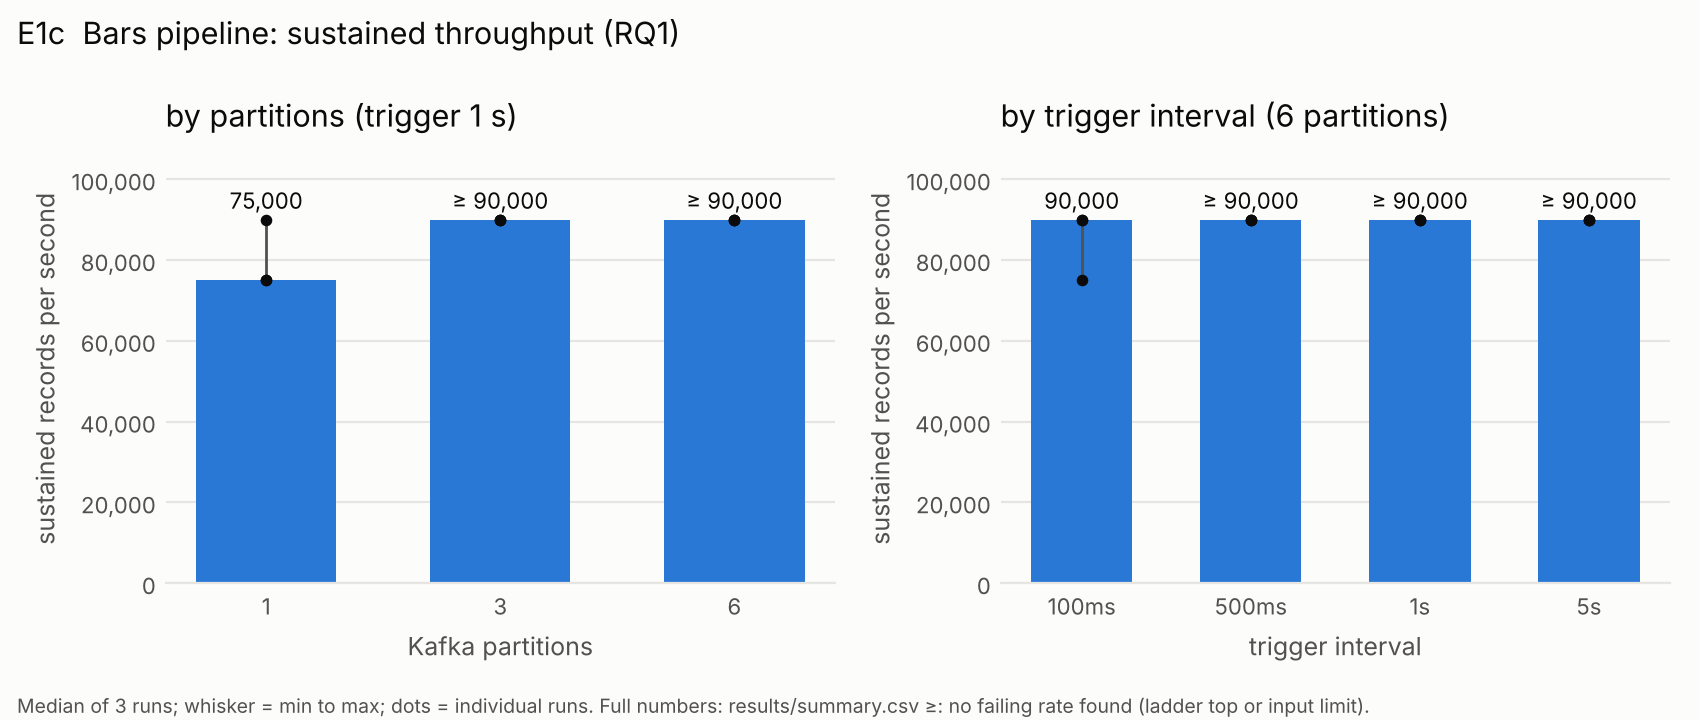
\includegraphics[width=0.85\textwidth]{e1c_sustained_throughput.png}
\caption{E1c: sustained throughput by partition count and trigger. Bars marked with a lower bound reached
our input limit before Spark's.}
\label{fig:e1c-tp}
\end{figure}

Bar latency runs from the window end plus the watermark to the moment the row is written.
Table~\ref{tab:e1c} gives the median p50.

\begin{table}[H]
\centering\small
\caption{E1c: bar latency p50 in seconds. The two sweeps ran on different CPUs (machine B, 2.30~GHz, and
machine A, 2.10~GHz), so we compare values only within one row.}
\label{tab:e1c}
\begin{tabular}{@{}lrr@{}}
\toprule
Setting & 30,000 records/s & 60,000 records/s \\
\midrule
1, 3, 6 partitions, trigger 1 s (machine B) & 2.5, 2.4, 2.5 & 2.4, 2.1, 3.5 \\
Trigger 100 ms, 500 ms, 1 s, 5 s, 6 partitions (machine A) & 2.2, \textbf{1.7}, 2.9, 7.2 & 6.4, 5.7, \textbf{4.9}, 8.7 \\
\bottomrule
\end{tabular}
\end{table}

The best trigger depends on the load. At 30,000 records per second a 500 ms trigger is fastest. At
60,000 a batch takes about two seconds whatever the trigger (batch duration p50 2.4 s at 100 ms, 2.1 s
at 500 ms, 2.0 s at 1 s), so a shorter trigger no longer starts batches sooner and only adds
per-batch overhead. There 1 s wins. A 5 s trigger always waits the longest. Below saturation the partition
count matters little, and at 60,000 six partitions on four cores cost more than three, because each
batch has more tasks and more state-store work. See Figures~\ref{fig:e1c-30} and~\ref{fig:e1c-60}.

\begin{figure}[H]
\centering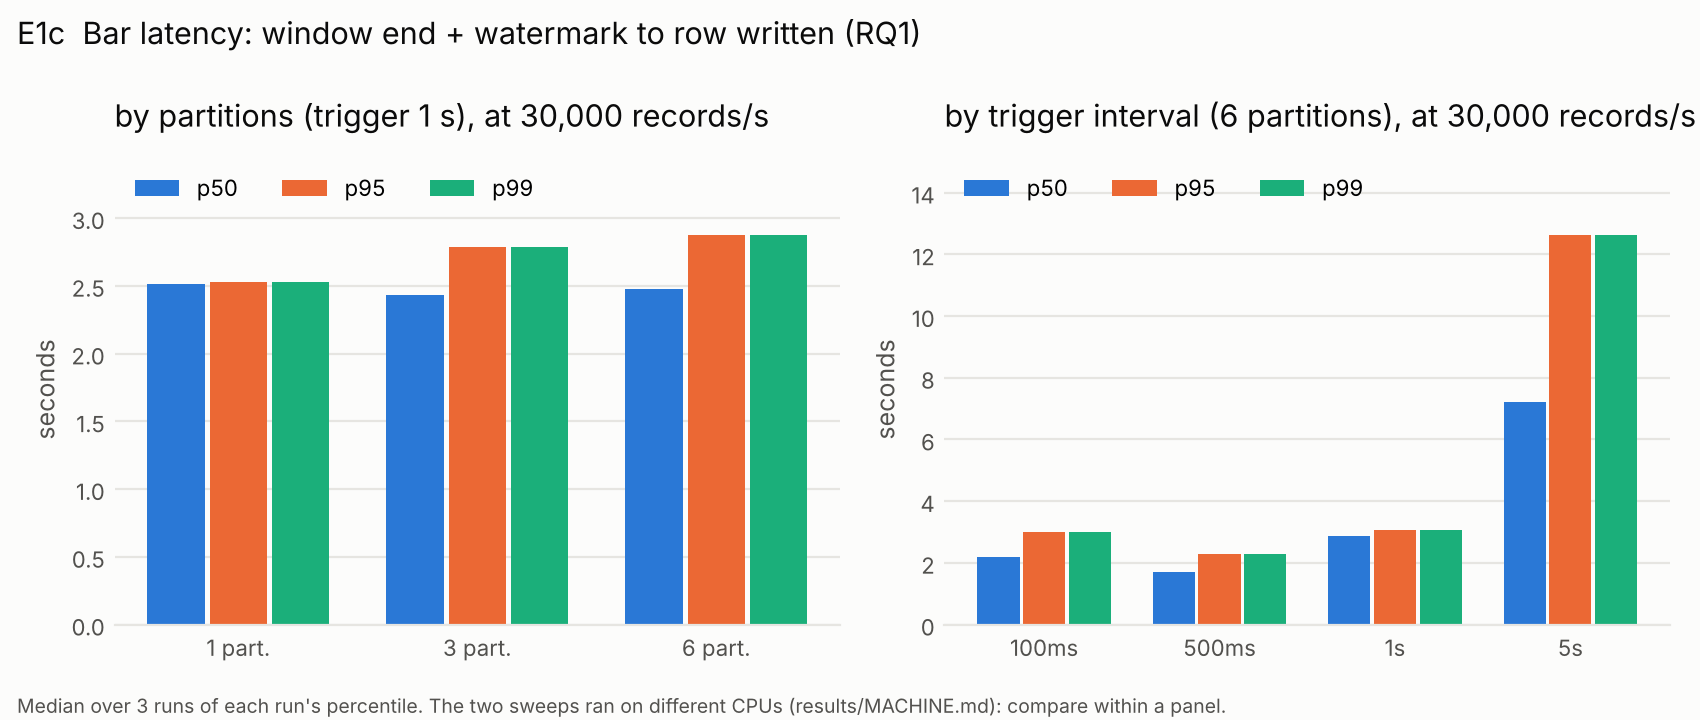
\includegraphics[width=0.85\textwidth]{e1c_bar_latency_30k.png}
\caption{E1c: bar latency at 30,000 records per second.}
\label{fig:e1c-30}
\end{figure}
\begin{figure}[H]
\centering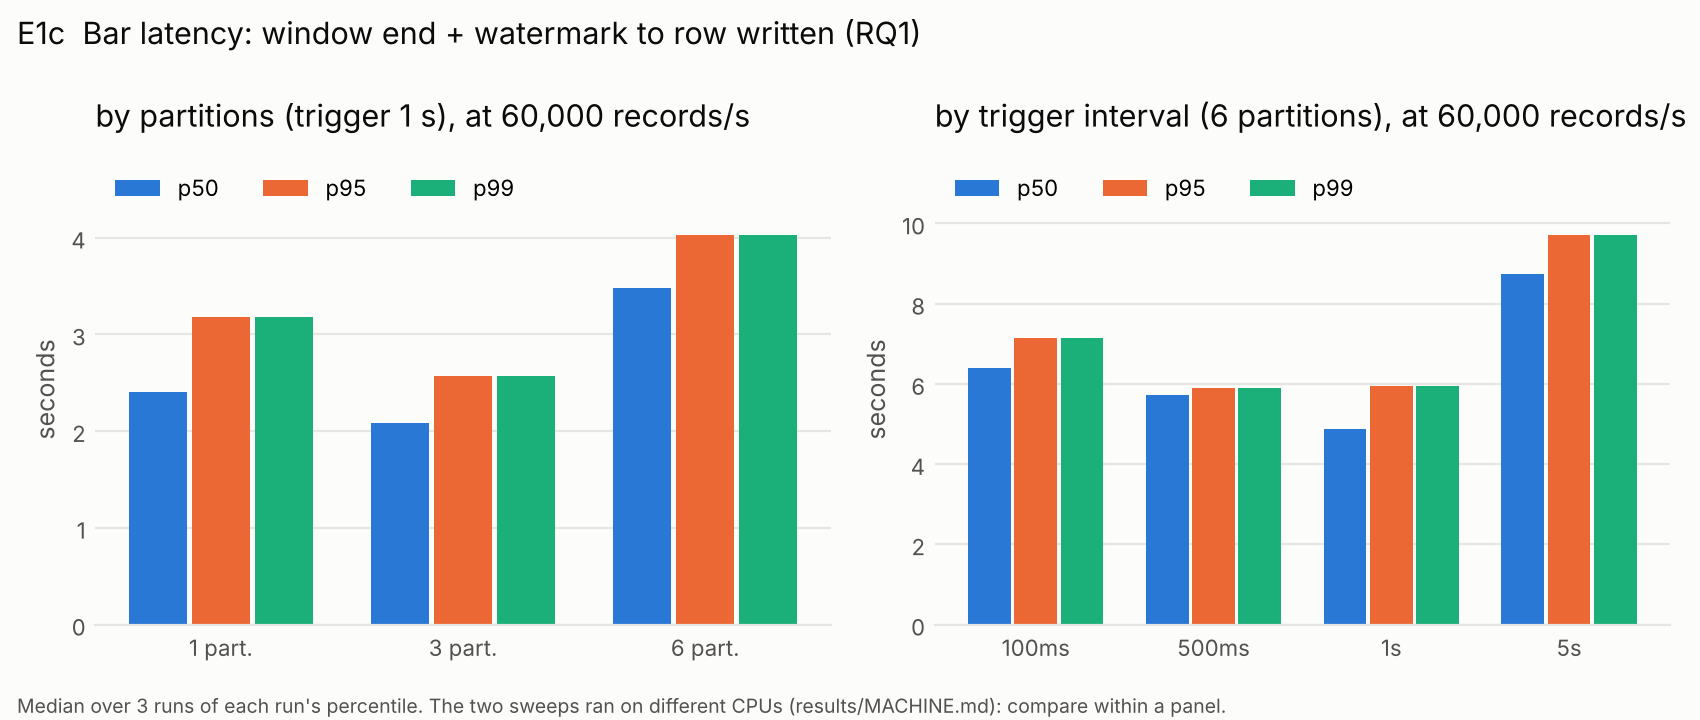
\includegraphics[width=0.85\textwidth]{e1c_bar_latency_60k.png}
\caption{E1c: bar latency at 60,000 records per second.}
\label{fig:e1c-60}
\end{figure}

\subsection{E2: broker crash (RQ2)}
We killed the broker that led partition 0 halfway through a 40-minute virtual run, with acks=1, with
acks=all, and with acks=all but no idempotence. No acknowledged trade was lost in any of the 12 kills.

With acks=all, writes stalled for 9.3 s [8.1 to 9.5] on every partition. The longest gap with no
acknowledgement anywhere was 9.1 s. The reason is that the dead broker stays in every partition's ISR
until the controller fences it, which takes the 9 s \code{broker.session.timeout.ms}. With acks=1 only the
partitions the dead broker led stalled, for 10.3 s [9.3 to 12.4], and the other partitions kept
acknowledging (longest gap anywhere 0.08 s). No duplicates appeared in these runs, even without
idempotence, although an earlier fault check did produce one (Section~\ref{sec:challenges}). A dry run
at a different rate did lose 2 acknowledged trades with acks=1, so loss is possible but rare.

One of the three runs without idempotence produced 33 wrong bars in a single minute even though Kafka
held every trade. The partitions resumed 3.8 s apart, the experiment's tenfold time compression turned
that into far more than the 10 s watermark, and Spark dropped those trades as late. This is a
real interaction between failover and watermarks, and we come back to it in Section~\ref{sec:limits}.
Figure~\ref{fig:e2} shows the stalls.

\begin{figure}[H]
\centering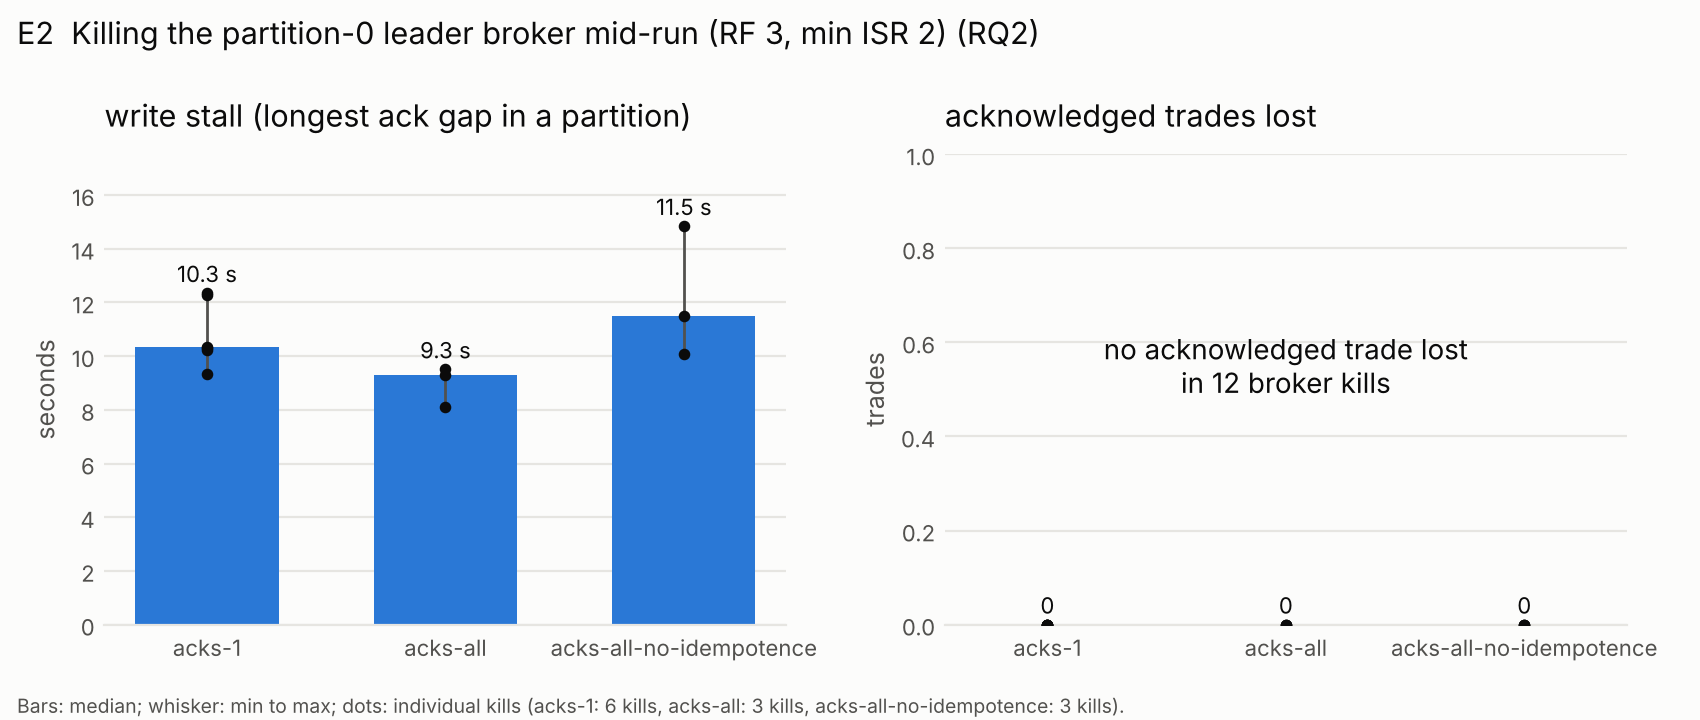
\includegraphics[width=0.9\textwidth]{e2_broker_crash.png}
\caption{E2: write stall and lost trades after a leader kill.}
\label{fig:e2}
\end{figure}

\subsection{E3: Spark crash (RQ2)}
We sent SIGKILL to the Spark container and restarted it at once on the same checkpoint. The first new bar
appeared 12.8 s [12.6 to 12.9] later in deterministic replay and 14.6 s [14.2 to 14.9] later on a live
stream, and the output was exact in all six runs. Almost all of that time is JVM and Spark start-up:
the first completed batch came 12.8 to 13.4 s after the restart. See Figure~\ref{fig:e3}.

\begin{figure}[H]
\centering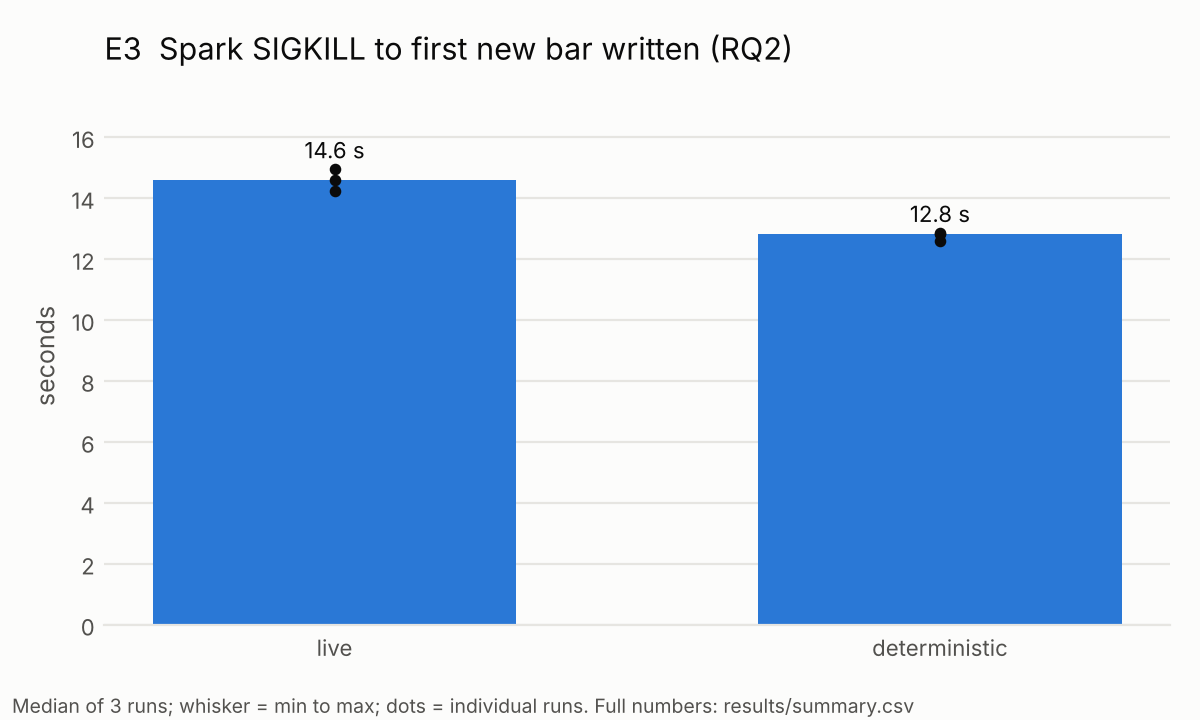
\includegraphics[width=0.7\textwidth]{e3_spark_recovery.png}
\caption{E3: time from the kill to the first new bar.}
\label{fig:e3}
\end{figure}

\subsection{E4: cost of exactly-once output (RQ3)}
We made Spark kill itself after the database commit and before Spark recorded the batch, so the restart
replays a batch that is already in the database. With plain inserts this left 300 duplicate bar rows in every
run, and with upserts none (three runs each). Without a crash, at 2,000 records per second, we could
not measure a cost for upserting. Batch duration p50 was 460 ms for inserts and 451 ms for upserts. Bar
latency p50 was 1.7 s [1.5 to 1.9] against 2.1 s [1.7 to 2.3], with overlapping ranges, and p99 was
2.45 s against 2.43 s. Both kept up. Figure~\ref{fig:e4} shows the results.

\begin{figure}[H]
\centering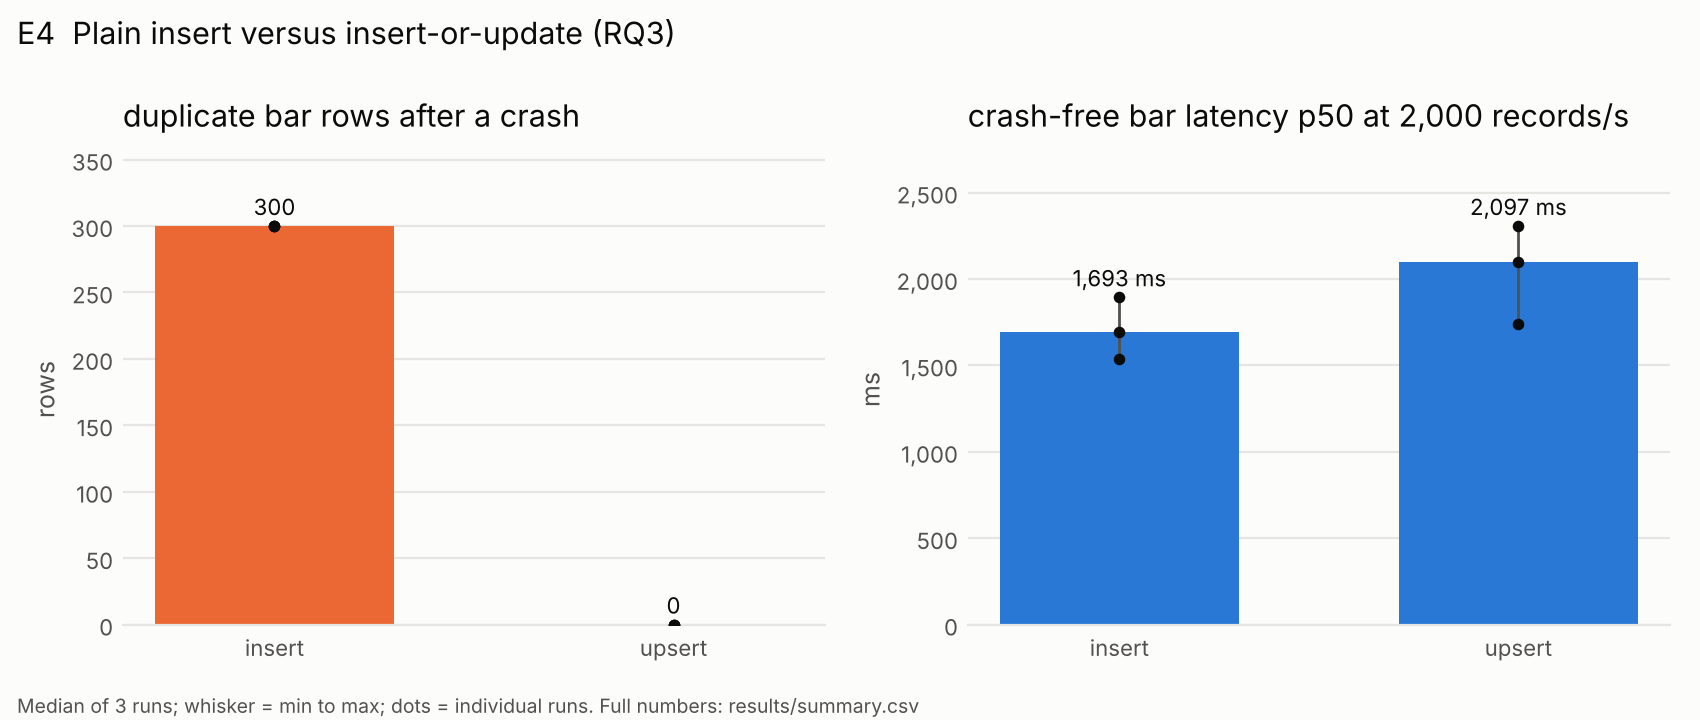
\includegraphics[width=0.9\textwidth]{e4_exactly_once.png}
\caption{E4: duplicate rows after a crash, and the cost of upserts without one.}
\label{fig:e4}
\end{figure}

\subsection{Live Coinbase run}
\label{sec:live}
We also ran the pipeline on live trades from Coinbase's public market-data feed for ten products (BTC, ETH,
SOL, XRP, DOGE, ADA, AVAX, LINK, LTC and BCH), on a Windows laptop with Docker Desktop, for more than 20
minutes. The producer connected to the feed, sent every trade to Kafka with acks=all, and saved a capture. The
dashboard filled with one-minute bars for all ten symbols, with Spark's lag at zero. No alert fired, which is
expected: live prices rarely move three standard deviations from their previous 30 one-minute returns, while the
synthetic data injects such shocks on purpose. After stopping the producer we ran the verifier against the
topic's own contents, because no generator file exists for live data. All 230 bars matched exactly (none
missing, extra, duplicated or different), and there were no alerts to match.

%------------------------------------------------------------------------------------------------
\section{Discussion: reproduction and extension}
\paragraph{Reproduction (a).} Batching raises producer throughput by more than an order of magnitude,
as Kreps et al.\ found, so the shape holds. Our unbatched rate is lower than theirs because every
one-record request is a round trip on a single shared four-core machine, and our batched rates are
higher because the producer and the CPU are newer. The paper used two dedicated 8-core machines, and we
approximate a batch of $n$ messages as $n \times 200$ bytes, since the Java producer sizes batches in bytes.

\paragraph{Reproduction (b).} Continuous processing gives much lower latency (tens of milliseconds
against hundreds) up to a saturation point, past which its latency climbs steeply, while micro-batch
sustains a higher input rate. The shape matches Armbrust et al. Their continuous latency was about
1 ms, and ours is tens of milliseconds because ours includes the producer's batching (\code{linger.ms}
of 5), a Kafka write with acks=all on three replicas, and the sink's own producer. The limit of one
core per partition on four cores is the constraint the paper describes, and we hit it.

\paragraph{Extension.} For RQ2, with replication factor 3 and a minimum ISR of 2, no acknowledged trade
was lost in 12 leader kills. The price of acks=all is a stall of about 9 s on every partition until the
dead broker is fenced. Acks=1 confines the stall to the dead broker's partitions but can lose
acknowledged writes, which we saw once, in a dry run. Spark recovers from its own crash in 13 to 15 s
with exact output. For RQ3, plain inserts are wrong after a crash (300 duplicate rows every time), and upserts
are exact at no cost we could measure at 2,000 records per second.

%------------------------------------------------------------------------------------------------
\section{Challenges}
\label{sec:challenges}
\begin{enumerate}
  \item \textbf{Determinism against late data.} An unpaced replay squeezes 40 virtual minutes into a few
        seconds, so a few milliseconds of skew between partitions looked like more than the 10 s watermark
        and trades would have been dropped as late. We now preload the topic before Spark starts.
  \item \textbf{Duplicates from producer retries.} With acks=all but idempotence off, killing a leader made
        the producer write one trade twice, and the verifier caught the wrong bar. Idempotence is now the
        default, and E2 measures the difference.
  \item \textbf{Measuring a write stall.} Looking at all partitions together hid the acks=1 behavior.
        We now compute the stall per partition from timestamped acknowledgements.
  \item \textbf{JVM warm-up} made the first latencies about twenty times worse, so we discard a warm-up
        period.
  \item \textbf{Continuous mode needs a core per partition.} With 6 partitions on 4 cores, two partitions were
        never processed, with no error. Continuous runs use 4 partitions.
  \item \textbf{Crashing between two commits.} A SIGKILL sent to PID 1 inside a container is ignored. The fault
        hook needed an init process and a kill of the driver JVM from inside \code{foreachBatch}.
  \item \textbf{Floating-point equality.} Fractional crypto sizes summed in a different order differ in
        the last bits, so the verifier allows a relative $10^{-9}$ for volume only.
  \item \textbf{Versions and tooling.} We checked that Kafka 4.4, Spark 4.2, PostgreSQL 18 and Grafana 13
        exist before pinning them, and had to build images behind a TLS-inspecting proxy and around Docker
        Hub rate limits.
  \item \textbf{Live data access.} The cloud development environment could not reach the Coinbase feed, so we
        first tested the adapter against a fake server that follows the protocol, and from captured sessions. We
        later ran it on a laptop (Section~\ref{sec:live}). Getting the stack to start on Windows took four fixes
        (a Linux-only default path, a missing image build, and two host ports that Windows had reserved or
        another project was using).
\end{enumerate}

%------------------------------------------------------------------------------------------------
\section{Reproducibility}
\label{sec:repro}
The repository holds everything needed to repeat the work. \code{docker compose up} starts the pipeline
and the demo. Image tags and Python packages are pinned and locked. A golden dataset with a SHA-256
manifest lets \code{make golden} replay a known stream through Kafka and Spark and check every bar and
alert against the oracle. \code{make bench-all} runs every experiment (about 12 hours), and
\code{uv run python -m bench.summarize} rebuilds every table and figure from the raw runs. Each run stores
its parameters, versions, git commit and machine. Continuous integration runs the linter, the unit tests and
the PostgreSQL integration tests on every push. The README explains how to run each step.

%------------------------------------------------------------------------------------------------
\section{Limitations: what one machine can and cannot show}
\label{sec:limits}
All three brokers, Spark (\code{local[4]}), PostgreSQL, Grafana, the generator and the measuring harness
ran on one virtual machine with 4 CPUs and 16 GB. Every container shares those four cores, one disk and
the loopback network. Our results are therefore sound for what they compare on this machine and weak as
absolute numbers.

\subsection{Throughput}
\begin{itemize}
  \item \textbf{Components compete for the same CPUs.} A measured rate is the pipeline's capacity while the
        generator, three brokers and PostgreSQL also run. On a cluster Kafka, Spark and the producers would
        have their own cores and every rate here would probably be higher. We report sustained rates as
        properties of this machine, not as limits of Kafka or Spark.
  \item \textbf{Our input is itself a ceiling.} The Python generator tops out near 100,000 records per second
        while Spark runs beside it. ``At least 90,000'' and ``micro-batch kept up at 100,000'' mean that the
        pipeline did not saturate before our input did. The true maximum is unknown.
  \item \textbf{Partition scaling is capped by cores.} More partitions than cores did not help (E1b, E1c). That
        shows the four-core limit and says nothing about how Kafka scales. The benefits of partitions in
        production, such as consumers on many machines and many disks, cannot appear here.
  \item \textbf{No network cost.} Replication between brokers crosses the loopback interface, so the latency of
        acks=all, which waits for replicas over a real network, is understated. E1a also differs from the
        paper because producer and broker share cores, where the paper used two 8-core machines.
  \item \textbf{One disk and the page cache.} Kafka depends on sequential disk writes and the page cache.
        Three brokers on one volume cannot show per-broker disk limits, and we did not enable \code{fsync}.
  \item \textbf{Changing hardware.} The virtual machine's CPU changed from 2.30 to 2.10 GHz between two
        experiments. We added a baseline setting (\code{p6-1s-b}) and compare triggers only within one machine
        state. Three runs per setting give a range, not a confidence interval.
  \item \textbf{Synthetic data.} Every measurement uses the seeded generator. Live Coinbase data appears only
        in the demonstration and in the short run of Section~\ref{sec:live}.
\end{itemize}

\subsection{Fault tolerance}
\begin{itemize}
  \item \textbf{A killed container is not a failed node.} \code{docker kill} stops one broker process at once.
        It does not model a network partition, a slow or full disk, a failed rack, a lost machine, or two
        brokers failing together. With three brokers on one host, the host is a single point of failure that
        none of our experiments can survive.
  \item \textbf{Detection time is configuration, not network behavior.} The 9 s stall in E2 equals the
        controller's \code{broker.session.timeout.ms} of 9,000 ms. On a real network, detection also depends on
        latency, partitions and clocks, and the stall could be shorter if tuned, or longer. We measured how this
        configuration reacts to a clean kill, not how fast Kafka recovers in general.
  \item \textbf{We injected the favorable failure.} A crashed leader's followers hold identical data, so a
        minimum ISR of 2 with unclean election off loses nothing. A leader that stays up but is cut off from
        its followers would test those settings harder, and we cannot produce that here.
  \item \textbf{Spark recovery excludes a cluster.} \code{local[4]} has no executors to lose, no rescheduling and
        no network shuffle. E3 measures checkpoint recovery of the driver (JVM start, state restore and
        replay), which is real, but not recovery on a standalone, YARN or Kubernetes cluster.
  \item \textbf{Time compression magnifies skew.} The crash experiments run virtual time ten times faster than
        the wall clock. A failover skew of a few seconds between partitions became tens of seconds of event
        time and made the 10 s watermark drop trades in one run (Section~\ref{sec:results}). With real-time data
        the same skew is ten times smaller relative to the watermark, so the failure would be rarer. The
        lesson that the watermark must exceed the partition skew still holds.
  \item \textbf{One local database.} A single PostgreSQL on the same machine has no network round trip and no
        competing writers, so the upsert cost we measured at 2,000 records per second is a lower bound for a
        remote or shared database.
\end{itemize}

\subsection{What still holds}
The correctness results do not depend on the machine. The bars and alerts match the oracle in every run,
no acknowledged trade was lost, and the duplicate rows in E4 follow from the protocol: a crash between
the database commit and Spark's commit replays the batch. The relative comparisons made on one machine
state (batching against none, continuous against micro-batch, trigger intervals, insert against upsert)
are valid for that machine, and their shapes agree with the published papers. We described Kafka's
security features (TLS, SASL, ACLs) but did not measure them. The harness could be pointed at a
multi-node cluster to extend the study.

%------------------------------------------------------------------------------------------------
\section{Conclusion}
\paragraph{RQ1.} The processing mode sets the latency floor. Continuous processing answers in tens of
milliseconds but saturates between 40,000 and 80,000 records per second on four cores, while micro-batch
trades hundreds of milliseconds for at least 100,000 records per second. For the bars pipeline the
trigger should match the load: 500 ms at moderate load, 1 s at high load, and 5 s was never best. More
partitions than cores did not help.

\paragraph{RQ2.} With replication factor 3 and a minimum ISR of 2, no acknowledged trade was lost in 12
leader kills. Acks=all stalls all writes for about 9 s until the dead broker is fenced, and acks=1 stalls
only its partitions but can lose acknowledged writes. A failover can also make Spark drop trades as late
when the watermark is shorter than the skew between partitions. Spark recovers from its own crash in
about 13 to 15 s with exact output.

\paragraph{RQ3.} Exactly-once output needs an idempotent sink. Plain inserts duplicated 300 rows after
every crash between the database commit and Spark's commit, upserts duplicated none, and at 2,000 records
per second the upsert cost nothing measurable.

\bibliographystyle{unsrt}
\bibliography{references}

%------------------------------------------------------------------------------------------------
\appendix
\section{Configuration of each experiment}
\label{app:config}
These tables come from \path{docker-compose.yml}, the topic script, the generator's defaults and the
experiment definitions in \path{bench/experiments/}. Each run also stores its own parameters in
\path{config.json} next to its raw output.

\subsection{Settings shared by all experiments}
\begin{table}[H]
\centering\small
\caption{Stack settings.}
\begin{tabularx}{\textwidth}{@{}>{\raggedright\arraybackslash}p{3.2cm}Y@{}}
\toprule
Component & Setting \\
\midrule
Kafka brokers & Image \code{apache/kafka:4.4.0}; 3 nodes, each broker and controller (KRaft combined mode); heap 1 GB per broker; \code{default.replication.factor=3}; \code{min.insync.replicas=2}; \code{unclean.leader.election.enable=false}; \code{auto.create.topics.enable=false}; PLAINTEXT listeners; no \code{log.flush.*} override; failure detection at the defaults (session timeout 9,000 ms, heartbeat 2,000 ms). \\
Topics & \code{trades}: 6 partitions by default (set per experiment), RF 3, min ISR 2, retention 1 day. \code{passthrough\_out}: same partitions as \code{trades}, RF 3, min ISR 2, \code{LogAppendTime}, retention 1 day. \code{perf\_test}: 1 partition, RF 1, min ISR 1, retention 1 hour. \\
Spark & Image \code{spark:4.2.1-scala2.13-java17-python3-ubuntu} with the Kafka connector \code{spark-sql-kafka-0-10\_2.13:4.2.1}; \code{--master local[4]}; driver memory 2 GB; container limit 4 CPUs and 3 GB; \code{spark.sql.shuffle.partitions=4}; session time zone UTC; \code{failOnDataLoss=true}; checkpoints on a named volume. \\
Bars job & Trigger 1 s; watermark 10 s; sink mode upsert; \code{startingOffsets=earliest}. \\
Pass-through job & Micro-batch trigger 100 ms, or continuous with a 1 s checkpoint interval; \code{startingOffsets=latest}. \\
PostgreSQL & Image \code{postgres:18.6}. \\
Producer (\code{confluent-kafka}) & \code{linger.ms=5}; \code{batch.size=1000000}; \code{retries=2147483647}; \code{queue.buffering.max.messages=500000}; \code{acks=all} with \code{enable.idempotence=true}, except where an experiment says otherwise (idempotence cannot be combined with acks=1). \\
\bottomrule
\end{tabularx}
\end{table}

\subsection{Settings per experiment}
\begin{table}[H]
\centering\footnotesize
\caption{Per-experiment settings. ``Records/s'' is the input rate.}
\begin{tabularx}{\textwidth}{@{}>{\raggedright\arraybackslash}p{1.1cm}YYY@{}}
\toprule
 & Kafka & Spark & Producer and input \\
\midrule
E1a & \code{perf\_test}: 1 partition, RF 1, min ISR 1; topic recreated for each setting & None & \code{kafka-producer-perf-test} inside \code{kafka-1}, 10 million records of 200 bytes, unlimited rate, \code{acks=0}; \code{batch.size} 0, 2,000, 10,000, 20,000, 40,000 bytes; \code{linger.ms} 0 (batch 1) or 10 \\
E1b & \code{trades} and \code{passthrough\_out}: 4 partitions, RF 3, min ISR 2 & Pass-through job; continuous (1 s checkpoint) or micro-batch (100 ms trigger); \code{startingOffsets=latest} & Realtime, \code{acks=all}, idempotent; continuous at 5,000, 10,000, 20,000, 40,000 and 80,000 records/s for 120 s (20 s warm-up); micro-batch at 40,000, 80,000 and 100,000 for 300 s (30 s warm-up) \\
E1c & \code{trades}: 1, 3 or 6 partitions, RF 3, min ISR 2; recreated before each step & Bars job, upsert sink; trigger 100 ms, 500 ms, 1 s or 5 s; \code{startingOffsets=latest} & Realtime, \code{acks=all}, idempotent, no closing trade; 30,000, 60,000 and 90,000 records/s, 300 s per step, 70 s warm-up; settings p1, p3, p6 with a 1 s trigger, and p6 with 100 ms, 500 ms, 5 s, plus a repeat of p6 at 1 s \\
E2 & \code{trades}: 6 partitions, RF 3, min ISR 2; the leader of partition 0 killed at 50\% of the run & Bars job, trigger 1 s, \code{startingOffsets=earliest} & Virtual mode, seed 42, 40 virtual minutes at 10 times speed, 1.0 trades per symbol per virtual second; acks=all with idempotence (3 kills), acks=1 (6 kills), acks=all without idempotence (3 kills) \\
E3 & \code{trades}: 6 partitions, RF 3, min ISR 2 & Bars job; SIGKILL at 50\% of the stream (live) or after batch 5 (deterministic, \code{maxOffsetsPerTrigger=5000}); restart at once on the same checkpoint & Live: virtual mode, seed 42, 40 minutes at 10 times speed. Deterministic: golden dataset (60,163 trades) preloaded and replayed at maximum speed. \code{acks=all}, idempotent \\
E4 & \code{trades}: 6 partitions, RF 3, min ISR 2 & Bars job; sink insert (\code{bars\_plain}) or upsert (\code{bars}); crash runs use \code{FAULT\_AFTER\_BATCH=5} and \code{maxOffsetsPerTrigger=5000} & Crash runs: golden replay. Cost runs: realtime at 2,000 records/s for 300 s, 70 s warm-up, no crash \\
\bottomrule
\end{tabularx}
\end{table}

\section{Machine and versions}
\label{app:machine}
Runs started on 11 November 2026 and finished on 12 November 2026 (72 runs, none failed). The development
virtual machine was moved between physical hosts when it restarted, so two CPUs appear. Both are 4-vCPU Intel
Xeon virtual machines with 15.7 GB of memory, Docker 29.9.2 and Linux 6.18.44: machine A at 2.10 GHz and
machine B at 2.30 GHz. Table~\ref{tab:machines} says which experiments ran where, and results are compared
only within one machine.

\begin{table}[H]
\centering\small
\caption{Where each experiment ran.}
\label{tab:machines}
\begin{tabular}{@{}ll@{}}
\toprule
Machine & Settings \\
\midrule
A (2.10 GHz) & E1c p6-100ms, p6-500ms, p6-5s and p6-1s-b; E2 (all); E3 (all); E4 crash runs \\
B (2.30 GHz) & E1a (all); E1b (all); E1c p1-1s, p3-1s and p6-1s; E4 cost runs \\
\bottomrule
\end{tabular}
\end{table}

\noindent Software: Apache Kafka 4.4.0, Apache Spark 4.2.1 (PySpark, Python 3.10 in the image), PostgreSQL
18.6, Grafana 13.3.0; on the host Python 3.13, confluent-kafka 2.16.1, psycopg 3.3.8, numpy 2.5.3 and
pandas 3.0.5, all pinned in the repository's lock file.

%   3. Add the packages below to the template's preamble if it does not load them already:
%        booktabs, tabularx, array, graphicx, float, caption, enumitem, tikz (with libraries
%        positioning, arrows.meta, shapes.geometric, fit, backgrounds), xurl, hyperref
%        and this macro:   \newcommand{\code}[1]{\texttt{#1}}
%        and this column type:   \newcolumntype{Y}{>{\raggedright\arraybackslash}X}
%        and:   \graphicspath{{figures/}}
%   4. If the template sets up its own bibliography, delete the two lines near the end of this file
%      (\bibliographystyle and \bibliography) and keep the template's.
%
% report/main.tex is a ready-made wrapper that does exactly this, so it compiles on its own.

\begin{abstract}
Trading desks want per-minute summaries and alerts within seconds of each trade. We built that
pipeline from Apache Kafka 4.4 (three brokers, KRaft) and Spark 4.2 Structured Streaming (PySpark).
It writes one-minute open, high, low, close and volume-weighted average price (VWAP) bars and
three-sigma alerts to PostgreSQL, shows them in Grafana, and starts with one \code{docker compose up}.
A seeded generator makes the correct output known exactly, so we check every run bar by bar. We
reproduce two published results, producer batching (Kreps et al., Figure 4) and continuous versus
micro-batch latency (Armbrust et al., Figure 7), and add what neither paper measured: whether the output
stays correct when a broker or the Spark job crashes, and what exactly-once output costs. No
acknowledged trade was lost in 12 broker crashes. Spark recovered from its own crash in about 14
seconds with exact output. Plain inserts left 300 duplicate rows after every crash, while upserts left
none and cost nothing we could measure at 2,000 trades per second. All measurements come from one
4-CPU machine, and Section~\ref{sec:limits} says what that does to the conclusions.
\end{abstract}

%------------------------------------------------------------------------------------------------
\section{Background and significance}
Market data arrives as a continuous stream of trades. A common design pairs a durable, partitioned
log that stores the events with a stream processor that reads the log and computes results over time
windows.

\paragraph{Apache Kafka.} Kafka~\cite{kreps2011,wang2015} is the log. A topic is split into
partitions, and each partition is an append-only file on a broker, written and read sequentially in
batches. Kreps et al.\ showed that this gives much higher throughput than traditional message
queues~\cite{kreps2011}. Kafka orders events only within a partition, so keying trades by symbol keeps
each symbol's trades in order. Each partition is copied to several brokers: a leader serves reads and
writes, and the followers that are caught up form the in-sync replica set (ISR). Whether an acknowledged
write survives a broker crash depends on three settings: the replication factor, the number of copies
the producer waits for (\code{acks}), and the minimum number of in-sync replicas~\cite{wang2015}. Kafka 4
keeps cluster metadata in its own Raft-based protocol (KRaft), so it no longer needs ZooKeeper.

\paragraph{Spark Structured Streaming.} Structured Streaming~\cite{armbrust2018} is the processor. It
treats a stream as an unbounded table and runs a normal SQL-style query over it incrementally, usually
in micro-batches, an approach that descends from discretized streams~\cite{zaharia2013}. It aggregates
over event-time windows and keeps intermediate state between batches. A watermark says how long Spark
waits for late events before it finalizes a window, an idea from the Dataflow model~\cite{akidau2015}.
Spark records each batch's Kafka offsets and its state in a checkpoint. Kafka can re-deliver from any
offset, so after a crash Spark re-runs exactly the unfinished batches, and an idempotent sink then makes
the result the same as if each event had been processed once. An experimental continuous mode lowers
latency, but it supports only per-record operations and delivers at least once.

\paragraph{Why test them together.} The papers promise high throughput from batched sequential I/O,
durability from replication, and exactly-once results from replay plus checkpoints. Each promise
depends on configuration and on how the two systems are connected. We test them on a financial
workload with a known correct answer, and we focus on the seam between the systems more than on either
one alone.

%------------------------------------------------------------------------------------------------
\section{Goals and objectives}
We set out to answer three research questions.
\begin{enumerate}[label=\textbf{RQ\arabic*.},leftmargin=*]
  \item How do the number of partitions, the trigger interval and the processing mode trade latency
        against throughput?
  \item Which Kafka settings prevent lost or duplicated data when a broker crashes, and how long does
        Spark take to recover from its own crash?
  \item What does exactly-once output cost compared with at-least-once output?
\end{enumerate}
The objectives are: (1) explain how Kafka, Spark and their integration work; (2) build a case-study
pipeline that starts with one command; (3) reproduce Kreps et al.\ Figure~4 and Armbrust et al.\
Figure~7, comparing the shape of each curve and not the absolute numbers; (4) extend both papers with
experiments they did not run, namely correctness under crashes and the cost of exactly-once output;
and (5) publish a repository that others can run, with pinned versions and scripted experiments.

%------------------------------------------------------------------------------------------------
\section{Architecture analysis}
\label{sec:arch}
Figure~\ref{fig:pipeline} shows the pipeline we built. A generator publishes trades, keyed by symbol,
to a topic with six partitions. Spark reads one task per partition, builds one-minute bars with a
10-second watermark, and writes each batch to PostgreSQL in one transaction. Grafana reads PostgreSQL.

\begin{figure}[H]
\centering
\resizebox{\textwidth}{!}{%
\begin{tikzpicture}[
  node distance=9mm and 8mm,
  box/.style={draw,rounded corners=2pt,align=center,inner sep=4pt,font=\small,minimum height=10mm},
  store/.style={draw,cylinder,shape border rotate=90,aspect=0.25,align=center,font=\small,minimum height=11mm,inner sep=3pt},
  arr/.style={-{Stealth[length=2mm]},thick},
  lab/.style={font=\scriptsize,align=center}]
  \node[box] (gen) {Generator\\(seeded, or\\Coinbase live)};
  \node[box,right=26mm of gen] (kafka) {Kafka, 3 brokers\\topic \code{trades}\\6 partitions, RF 3,\\min ISR 2};
  \node[box,right=26mm of kafka] (spark) {Spark\\\code{local[4]}, 1 s trigger\\watermark 10 s,\\1-minute windows};
  \node[store,right=30mm of spark] (pg) {PostgreSQL\\bars, alerts};
  \node[box,right=12mm of pg] (graf) {Grafana};
  \node[store,below=8mm of spark] (ck) {Checkpoint\\volume};
  \draw[arr] (gen) -- node[lab,above]{key = symbol} node[lab,below]{acks=all} (kafka);
  \draw[arr] (kafka) -- node[lab,above]{one task per} node[lab,below]{partition} (spark);
  \draw[arr] (spark) -- node[lab,above]{one transaction} node[lab,below]{per batch} (pg);
  \draw[arr] (pg) -- (graf);
  \draw[arr,dashed] (spark) -- node[lab,right]{offsets, state} (ck);
\end{tikzpicture}}
\caption{The pipeline. A separate pass-through job (not shown) copies \code{trades} to a second
topic for the latency experiments.}
\label{fig:pipeline}
\end{figure}

\subsection{Kafka}
Table~\ref{tab:kafka} lists the Kafka mechanisms we rely on and where each one shows up in the project.

\begin{table}[H]
\centering\small
\caption{Kafka mechanisms and their role in this project.}
\label{tab:kafka}
\begin{tabularx}{\textwidth}{@{}>{\raggedright\arraybackslash}p{3.1cm}YY@{}}
\toprule
Mechanism & How it works & In this project \\
\midrule
Partitions and ordering & A partition is an append-only log on a broker, written and read sequentially. Order holds only within a partition; the producer picks the partition by hashing the key. & \code{trades} has 6 partitions on 3 brokers. Key = symbol, so every symbol lands in one partition and stays in order (checked from the acknowledgement log). \\
Throughput design~\cite{kreps2011} & Batching many records per request, sequential disk I/O, the page cache, zero-copy transfer. & E1a reproduces the batching effect. \\
Retention & Records stay for a time or size limit whether or not they were read, so a consumer can re-read from any offset. & \code{trades} keeps one day. Replay after a crash depends on it. \\
Replication and ISR~\cite{wang2015} & A partition has a leader and followers. A write is committed when every in-sync replica has it. & RF 3, \code{min.insync.replicas=2}, unclean leader election off, so only an in-sync replica can become leader. \\
Producer \code{acks} & 0: no wait. 1: the leader only. all: every in-sync replica. & E2 kills a leader with acks=1 and acks=all. \\
Idempotent producer & The broker drops a retried batch it has already seen, using the producer id and a sequence number. & On by default with acks=all. Without it, a leader kill once duplicated a trade (Section~\ref{sec:challenges}). \\
KRaft & Metadata lives in a Raft-replicated log on controller nodes. & Three nodes, each broker and controller. \\
Consumer groups & Consumers with one \code{group.id} split a topic's partitions, and Kafka stores the group's committed offsets. & Used by our verifier and latency collectors. Spark does not use them (Section~\ref{sec:integration}). \\
Delivery guarantees & At most once, at least once, or exactly once (idempotent producer plus transactions inside Kafka). & End-to-end exactly-once here comes from Spark's replay plus an idempotent sink. \\
Security & TLS encrypts traffic, SASL authenticates clients, ACLs authorize operations. & Described, not measured. The stack runs PLAINTEXT on one machine, with Grafana and PostgreSQL bound to localhost. \\
\bottomrule
\end{tabularx}
\end{table}

\subsection{Spark Structured Streaming}
Table~\ref{tab:spark} does the same for Spark.

\begin{table}[H]
\centering\small
\caption{Spark mechanisms and their role in this project.}
\label{tab:spark}
\begin{tabularx}{\textwidth}{@{}>{\raggedright\arraybackslash}p{3.1cm}YY@{}}
\toprule
Mechanism & How it works & In this project \\
\midrule
Unbounded table~\cite{armbrust2018} & A streaming query is an ordinary DataFrame query that Spark runs incrementally. The optimizer turns it into an incremental plan with stateful operators. & The bars job is a \code{groupBy(window, symbol)} aggregation. \\
Micro-batch and triggers~\cite{zaharia2013} & A trigger starts a batch at fixed intervals; each batch reads the offsets that arrived since the last one. & Trigger 1 s by default. E1c varies it from 100 ms to 5 s. \\
Continuous processing & Long-running tasks handle one record at a time and checkpoint in epochs. Lower latency, but only map-like operations, at-least-once, and one core per input partition. & Cannot run the bars job. E1b runs a pass-through job in both modes. With 6 partitions on 4 cores, two partitions were never processed. \\
Event time and watermark~\cite{akidau2015} & Windows follow the record's event time. The watermark is the largest event time seen minus a delay. In append mode a window is emitted once, when the watermark passes its end. & One-minute tumbling windows, 10 s watermark. A closing trade for a reserved symbol advances the watermark past the last windows. \\
State store & Partial aggregates per window and key, written to the checkpoint every batch and dropped after the watermark passes. & Open, high, low, close (using \code{min\_by} and \code{max\_by} on time and trade id), volume, notional, count. \\
Checkpoint & \code{offsets/} (the range each batch will read, written before processing), \code{commits/} (finished batches), \code{state/}. & A named volume that survives \code{docker kill}. E3 and E4 depend on it. \\
Sinks & Append, update or complete output; \code{foreachBatch} hands each batch to user code; the Kafka sink is at least once. & Append mode with \code{foreachBatch} into PostgreSQL. The pass-through job uses the Kafka sink. \\
Monitoring & A \code{StreamingQueryListener} receives one progress event per batch. & Written to a \code{query\_progress} table that feeds the dashboard and the throughput tests. \\
\bottomrule
\end{tabularx}
\end{table}

\subsection{Integration}
\label{sec:integration}
\paragraph{Partitions become tasks.} The Kafka source plans one Spark task per Kafka partition in each
batch, so the partition count bounds parallelism. E1c compares 1, 3 and 6 partitions on 4 cores.

\paragraph{Offsets live in Spark's checkpoint, not in a consumer group.} Spark picks each batch's offset
range and writes it to the checkpoint before it processes anything. That ties the offsets to the batch
id and to a version of the state. A consumer group's committed offset cannot do that: it says
``consumed'', not ``consumed and reflected in state version $n$ and in output batch $n$''. After a
crash Spark reads exactly the uncommitted range again. This requires Kafka to still hold the data
(\code{failOnDataLoss=true} stops the query if it does not) and the checkpoint to match the topic, so our
harness always wipes both together.

\paragraph{Exactly-once output is replay plus an idempotent sink.} Replay delivers a crashed batch a
second time, and the sink must make the second write harmless. Each batch's bars and alerts go to
PostgreSQL in one transaction, using \code{INSERT ... ON CONFLICT (symbol, window\_start) DO UPDATE},
and the \code{written\_at} column is set only on the first insert. Figure~\ref{fig:batch} shows the order
of events in one batch. A crash anywhere before the commit record makes Spark run the batch again from
the same offsets, and the upsert absorbs it. E4 tests exactly that.

\begin{figure}[H]
\centering\small
\begin{tabularx}{\textwidth}{@{}rlY@{}}
\toprule
Step & Actor & Action \\
\midrule
1 & Spark driver & Ask Kafka for the latest offset of every partition. \\
2 & Spark driver & Write the planned offset range to the checkpoint (\code{offsets/n}). \\
3 & Spark tasks & Read that range, one task per partition, and update the aggregation state. \\
4 & Spark driver & Emit the windows the watermark has passed. \\
5 & Sink & In one transaction: upsert the bars, read the 31 previous bars of each symbol, upsert the alerts, commit. \\
6 & Spark driver & Write \code{commits/n} and state version $n$. \\
\bottomrule
\end{tabularx}
\caption{One micro-batch. A crash between steps 5 and 6 replays the batch.}
\label{fig:batch}
\end{figure}

\subsection{Failure behavior}
Table~\ref{tab:failure} lists each failure we injected or considered and what the experiments showed.

\begin{table}[H]
\centering\small
\caption{Failure behavior and where we measured it.}
\label{tab:failure}
\begin{tabularx}{\textwidth}{@{}>{\raggedright\arraybackslash}p{3.6cm}Yl@{}}
\toprule
Failure & What happens & Measured in \\
\midrule
Leader broker killed, acks=all & Writes to every partition stall until the controller fences the dead broker and removes it from the ISR; then they continue. No acknowledged trade is lost. The stall matches \code{broker.session.timeout.ms} (9,000 ms) plus up to one heartbeat interval. & E2 \\
Leader broker killed, acks=1 & Only the partitions the dead broker led stall. Records it had acknowledged but not yet replicated can be lost when a follower takes over; not every kill loses data. & E2 \\
Producer retry without idempotence & A retried batch can be written twice. & E2, Section~\ref{sec:challenges} \\
Spark killed & Spark restarts from the checkpoint. Recovery time is mostly JVM and Spark start-up. Output stays exact with the upsert sink. & E3 \\
Spark killed after the sink commits & Spark replays the batch: duplicates with plain inserts, none with upserts. & E4 \\
Topic recreated under a checkpoint & \code{failOnDataLoss=true} stops the query instead of skipping data. & Harness procedure \\
\bottomrule
\end{tabularx}
\end{table}

\subsection{Design choices}
Several choices trade one property for another. A shorter watermark lowers bar latency but drops more
late trades, and because we measure latency from the window end plus the watermark, the watermark
adds directly to the time to result. A shorter trigger lowers latency but adds per-batch overhead
(E1c). More partitions add parallel tasks but also state-store and planning work on four cores. Setting
acks=all with a minimum ISR of 2 survives one broker failure at the price of a write stall while the
ISR shrinks (E2). We read the alert history back from PostgreSQL, which keeps the Spark job a plain
windowed aggregation, at the cost of one indexed query per batch. Running Spark as \code{local[4]} in one
container matches the 4-core setup of Armbrust et al.\ and our memory budget, but it is not a test of
distributed Spark.

%------------------------------------------------------------------------------------------------
\section{Features exercised}
\begin{table}[H]
\centering\small
\caption{Each feature, how the pipeline uses it, and what demonstrates it.}
\begin{tabularx}{\textwidth}{@{}>{\raggedright\arraybackslash}p{3.4cm}YY@{}}
\toprule
Feature & Use in the pipeline & Demonstrated by \\
\midrule
Partitioned, keyed log & 6 partitions, key = symbol, per-symbol order & Acknowledgement-log check; E1c \\
Replication and acks & RF 3, min ISR 2, acks=all, idempotent producer & E2 \\
Event-time windows and watermark & 1-minute bars, 10 s watermark, append mode & 4,000 bars match the oracle exactly \\
Stateful lookback & Alert when the log return is more than 3 standard deviations from the previous 30 bars & 23 of 23 expected alerts; 20 of 20 injected shocks found \\
Checkpoint recovery & Restart from offsets and state after SIGKILL & E3 \\
Exactly-once output & One transaction per batch, upsert on (symbol, minute) & E4 \\
Continuous processing & Kafka-to-Kafka pass-through & E1b \\
Monitoring & Progress listener to \code{query\_progress}, Grafana dashboard & Live dashboard \\
\bottomrule
\end{tabularx}
\end{table}

%------------------------------------------------------------------------------------------------
\section{Case study: the market-data pipeline}
\paragraph{Generator.} A seeded generator makes random-walk prices for 100 symbols. The busiest symbol
trades about ten times as often as the quietest, sizes are log-normal, and permanent price shocks of
1.5\% to 3\% happen at known times after a 30-bar warm-up, so we know which alerts must fire. It has
virtual, realtime and replay modes and writes a per-trade acknowledgement log. A fourth mode reads live
trades from Coinbase, with capture and replay as a fallback.

\paragraph{Spark job.} The job parses the JSON with an explicit schema and groups by symbol and
one-minute window. Open and close come from \code{min\_by} and \code{max\_by} ordered by event time and
trade id, so they do not depend on arrival order. VWAP uses \code{try\_divide} because Spark 4 raises an
error on division by zero.

\paragraph{Alert rule.} Our proposal says an alert fires when a price change is more than three
standard deviations from that symbol's average over the previous 30 bars. We read ``price change'' as
the bar-to-bar log return of the close. For each bar we take the 30 previous returns, compute their
mean and sample standard deviation, and alert when the new return differs from the mean by more than
three standard deviations. A symbol with fewer than 31 bars, or with zero variance, never alerts.

\paragraph{Sink and dashboard.} Each batch is one PostgreSQL transaction (Section~\ref{sec:integration}).
Grafana shows candlesticks, VWAP, alerts and Spark's own progress metrics.

\paragraph{Verification.} We treat verification as part of the system. An oracle
(\path{tools/gen_sample_dataset.py}, copied into \path{verify/reference.py}) computes the exact expected bars
and alerts. The verifier compares every bar (open, high, low and close exactly, VWAP within $10^{-6}$)
and every alert, and a second verifier compares the producer's acknowledgement log with the contents of
the topic. A run therefore passes or fails, including every crash experiment. The golden dataset has
60,163 trades, 4,000 bars, 23 alerts and 20 shocks, and its SHA-256 hashes are in a manifest.

%------------------------------------------------------------------------------------------------
\section{Experiments and results}
\label{sec:results}
\paragraph{Setup.} All experiments ran on one virtual machine with 4 CPUs, 16 GB of memory and Docker,
alone on it, three runs per setting (six kills for E2 with acks=1). Latency is the median over runs of
each run's p50, p95 and p99. Sustained throughput is the highest input rate at which Spark keeps up
over a five-minute run. We drop a warm-up period from every latency measurement, because JVM
start-up made the first seconds about twenty times slower. Ranges in brackets are the minimum and
maximum over runs. The machine and versions are in Appendix~\ref{app:machine}, and the Kafka, Spark
and producer settings of every experiment are in Appendix~\ref{app:config}.

\subsection{E1a: producer batching (reproduction of Kreps et al., Figure 4)}
We ran Kafka's own producer performance tool with acks=0, 10 million records of 200 bytes, and one
partition with no replication, as the paper did, varying the batch size.

\begin{table}[H]
\centering\small
\caption{E1a: producer throughput against batch size (median of 3 runs).}
\label{tab:e1a}
\begin{tabular}{@{}lrrrrr@{}}
\toprule
Batch size (messages) & 1 & 10 & 50 & 100 & 200 \\
\midrule
Records per second & 19,798 & 154,909 & 525,376 & 739,153 & 848,033 \\
\bottomrule
\end{tabular}
\end{table}

Batching raised throughput 26 times from 1 to 50 messages per batch. The paper reports about 8 times,
from roughly 50,000 to 400,000 messages per second. With acks=0 the tool's latency column means
nothing, so we do not report it. See Figure~\ref{fig:e1a}.

\begin{figure}[H]
\centering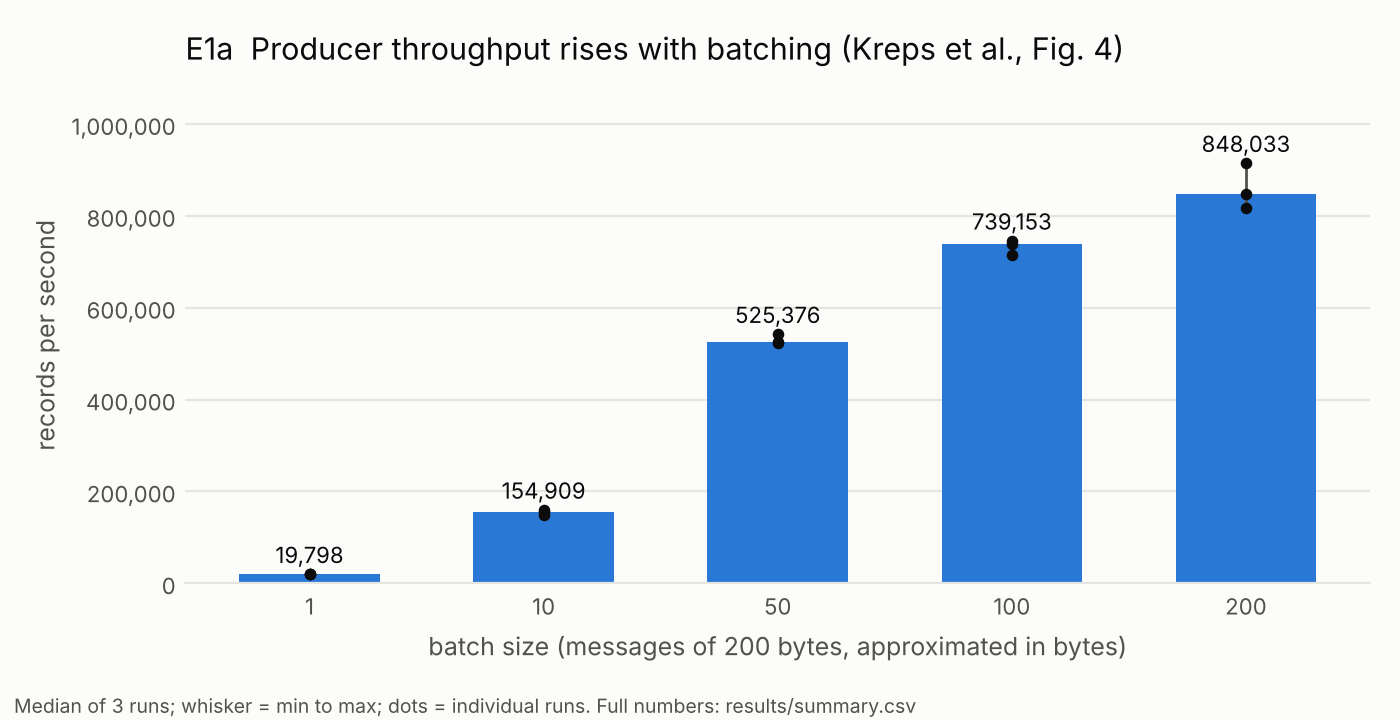
\includegraphics[width=0.8\textwidth]{e1a_producer_batching.png}
\caption{E1a: batching raises producer throughput.}
\label{fig:e1a}
\end{figure}

\subsection{E1b: continuous versus micro-batch (reproduction of Armbrust et al., Figure 7)}
A stateless pass-through job copies one topic to another. In continuous mode with 4 partitions, median
latency was 43 to 83 ms from 5,000 to 40,000 records per second (p99 0.3 to 0.9 s). At 80,000 records per
second its four tasks saturated: p50 rose to 1.8 s and p99 to 6.9 s. Micro-batch mode with a 100 ms
trigger kept up with the highest rate we could generate, at least 100,000 records per second, with
p50 between 0.27 and 0.62 s. See Figure~\ref{fig:e1b}.

\begin{figure}[H]
\centering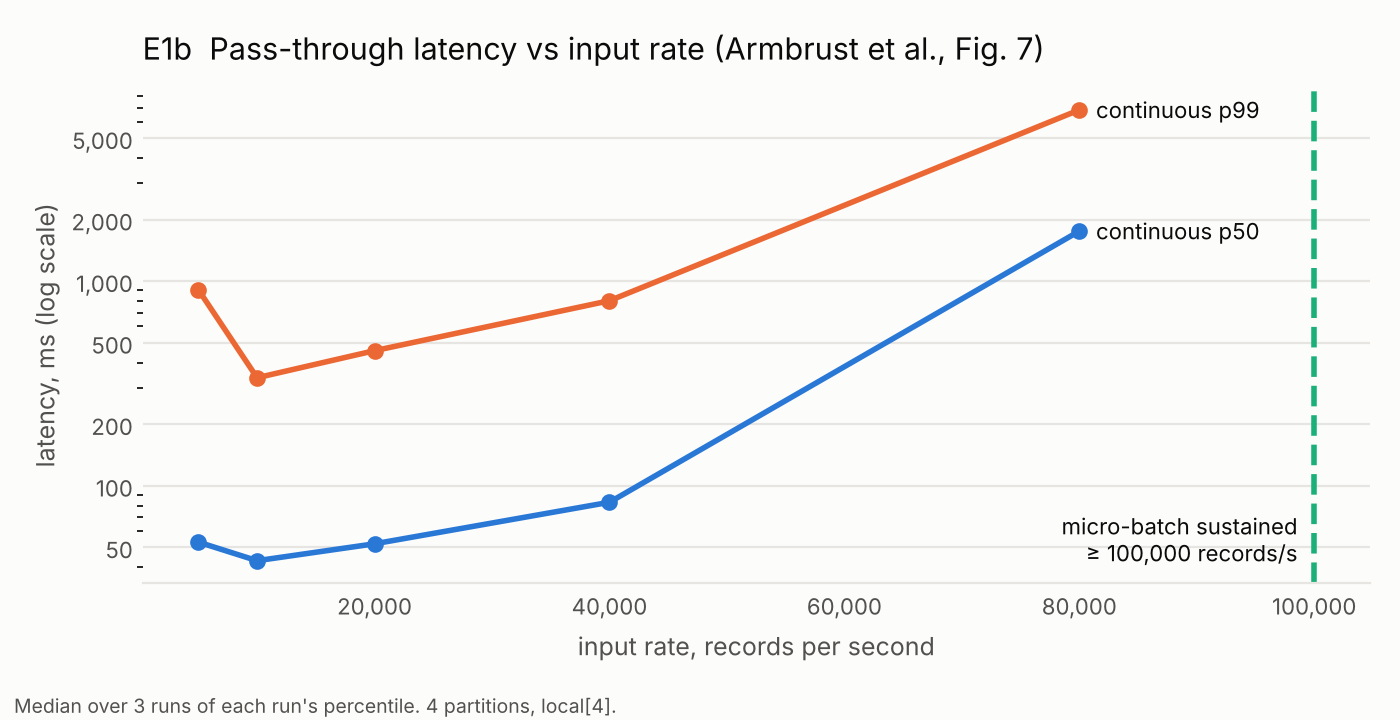
\includegraphics[width=0.85\textwidth]{e1b_continuous_vs_microbatch.png}
\caption{E1b: continuous mode has the lower latency until it saturates; micro-batch sustains a higher rate.}
\label{fig:e1b}
\end{figure}

\subsection{E1c: partitions and trigger interval (RQ1)}
Here we ran the real bars job in five-minute steps at 30,000, 60,000 and 90,000 records per second.
One partition sustained 75,000 records per second (one of three runs passed 90,000). Three and six
partitions, and every trigger from 500 ms to 5 s, sustained at least 90,000, which is the most our
generator could supply while sharing four cores with Spark. The 100 ms trigger reached its limit in one run of
three, at 75,000. Figure~\ref{fig:e1c-tp} shows this.

\begin{figure}[H]
\centering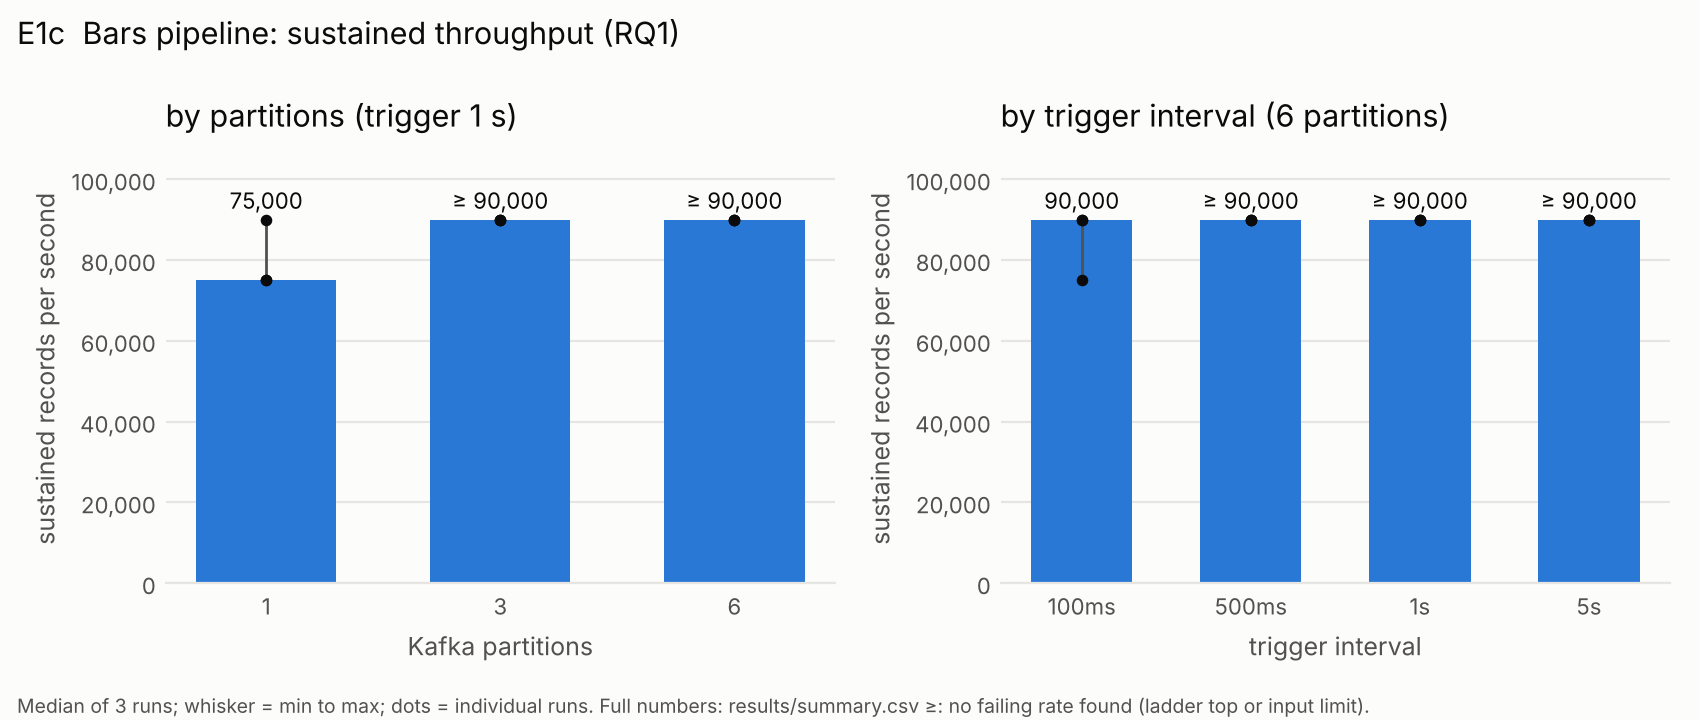
\includegraphics[width=0.85\textwidth]{e1c_sustained_throughput.png}
\caption{E1c: sustained throughput by partition count and trigger. Bars marked with a lower bound reached
our input limit before Spark's.}
\label{fig:e1c-tp}
\end{figure}

Bar latency runs from the window end plus the watermark to the moment the row is written.
Table~\ref{tab:e1c} gives the median p50.

\begin{table}[H]
\centering\small
\caption{E1c: bar latency p50 in seconds. The two sweeps ran on different CPUs (machine B, 2.30~GHz, and
machine A, 2.10~GHz), so we compare values only within one row.}
\label{tab:e1c}
\begin{tabular}{@{}lrr@{}}
\toprule
Setting & 30,000 records/s & 60,000 records/s \\
\midrule
1, 3, 6 partitions, trigger 1 s (machine B) & 2.5, 2.4, 2.5 & 2.4, 2.1, 3.5 \\
Trigger 100 ms, 500 ms, 1 s, 5 s, 6 partitions (machine A) & 2.2, \textbf{1.7}, 2.9, 7.2 & 6.4, 5.7, \textbf{4.9}, 8.7 \\
\bottomrule
\end{tabular}
\end{table}

The best trigger depends on the load. At 30,000 records per second a 500 ms trigger is fastest. At
60,000 a batch takes about two seconds whatever the trigger (batch duration p50 2.4 s at 100 ms, 2.1 s
at 500 ms, 2.0 s at 1 s), so a shorter trigger no longer starts batches sooner and only adds
per-batch overhead. There 1 s wins. A 5 s trigger always waits the longest. Below saturation the partition
count matters little, and at 60,000 six partitions on four cores cost more than three, because each
batch has more tasks and more state-store work. See Figures~\ref{fig:e1c-30} and~\ref{fig:e1c-60}.

\begin{figure}[H]
\centering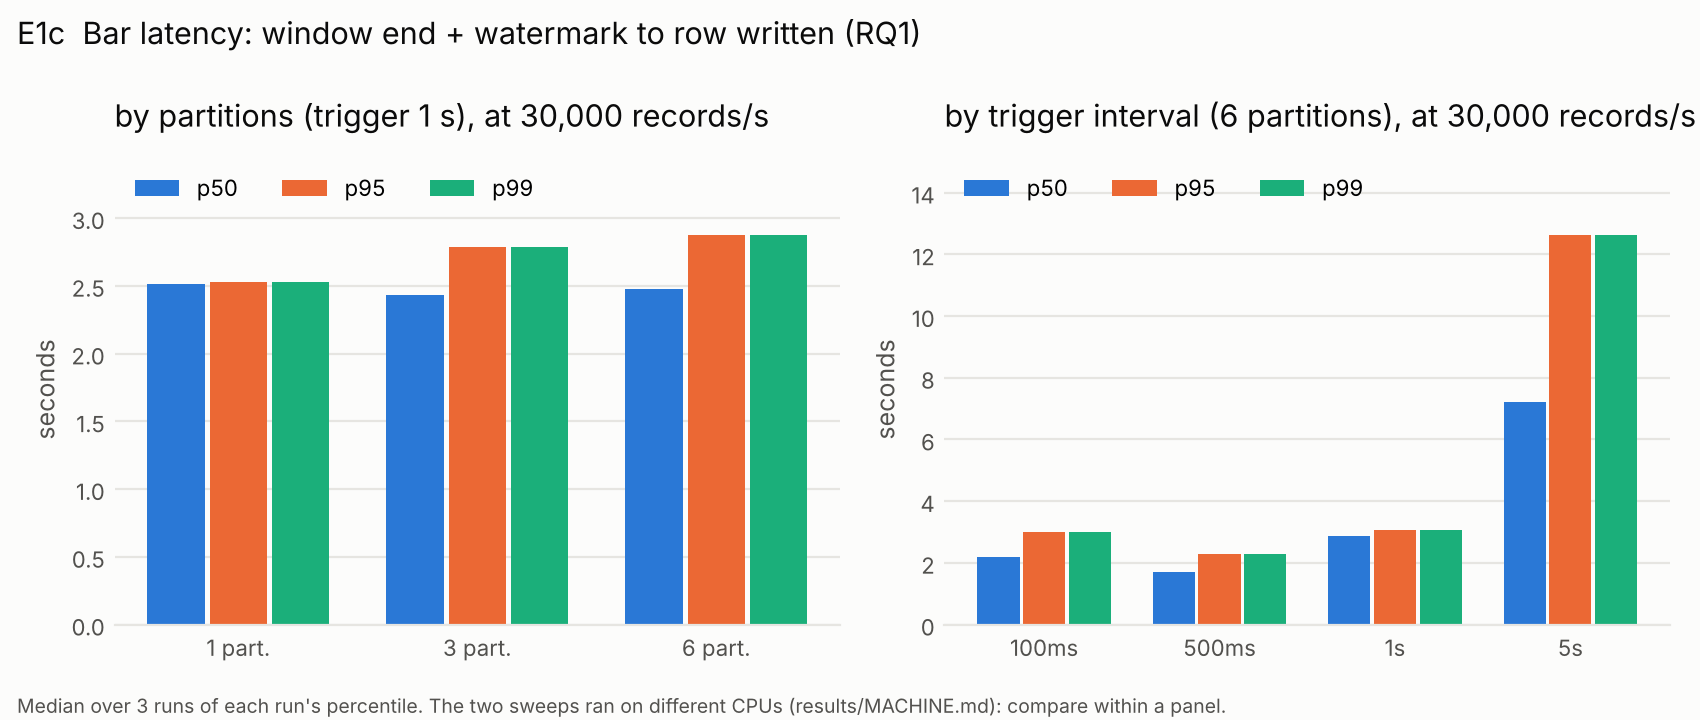
\includegraphics[width=0.85\textwidth]{e1c_bar_latency_30k.png}
\caption{E1c: bar latency at 30,000 records per second.}
\label{fig:e1c-30}
\end{figure}
\begin{figure}[H]
\centering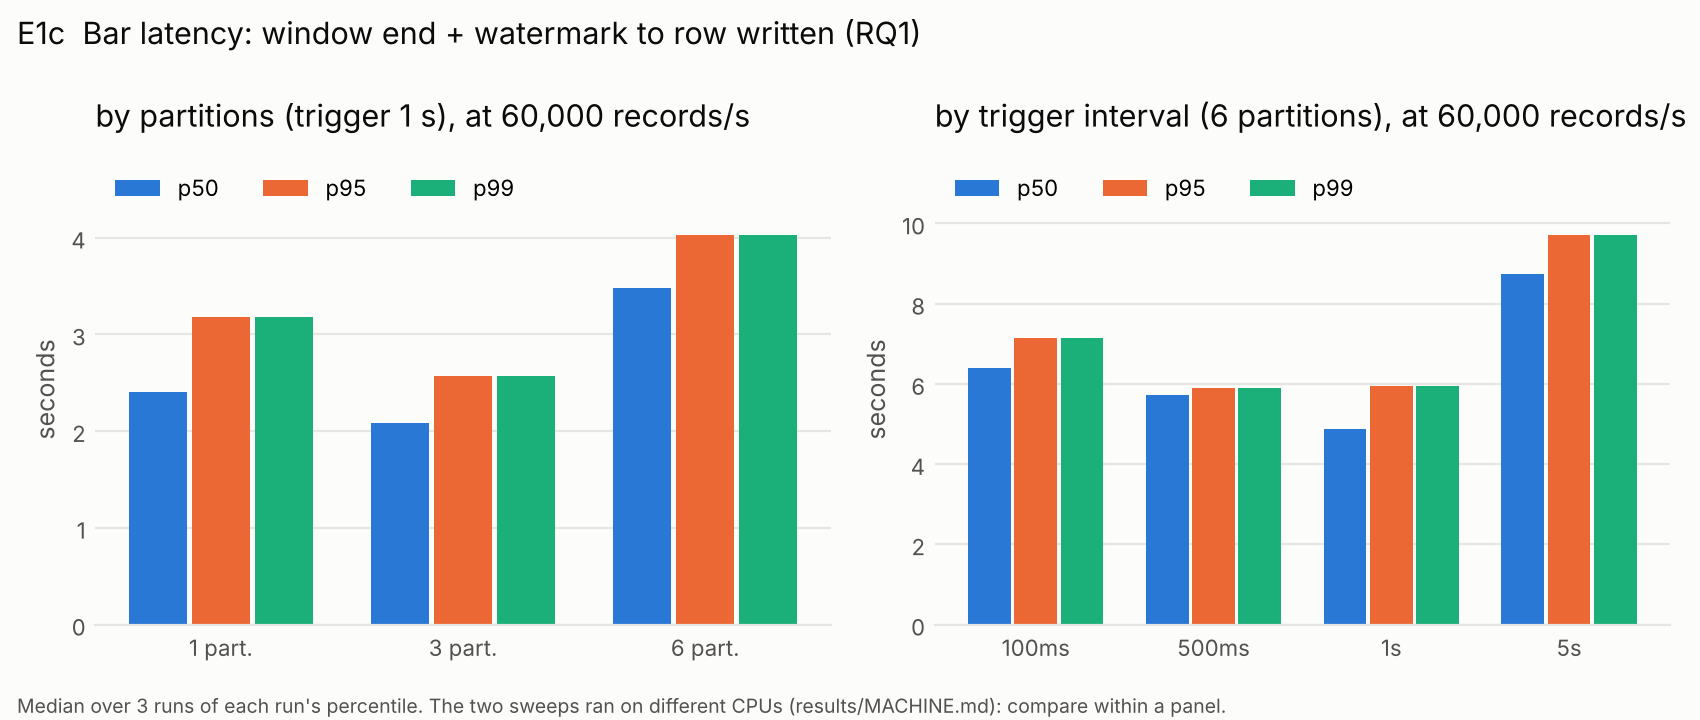
\includegraphics[width=0.85\textwidth]{e1c_bar_latency_60k.png}
\caption{E1c: bar latency at 60,000 records per second.}
\label{fig:e1c-60}
\end{figure}

\subsection{E2: broker crash (RQ2)}
We killed the broker that led partition 0 halfway through a 40-minute virtual run, with acks=1, with
acks=all, and with acks=all but no idempotence. No acknowledged trade was lost in any of the 12 kills.

With acks=all, writes stalled for 9.3 s [8.1 to 9.5] on every partition. The longest gap with no
acknowledgement anywhere was 9.1 s. The reason is that the dead broker stays in every partition's ISR
until the controller fences it, which takes the 9 s \code{broker.session.timeout.ms}. With acks=1 only the
partitions the dead broker led stalled, for 10.3 s [9.3 to 12.4], and the other partitions kept
acknowledging (longest gap anywhere 0.08 s). No duplicates appeared in these runs, even without
idempotence, although an earlier fault check did produce one (Section~\ref{sec:challenges}). A dry run
at a different rate did lose 2 acknowledged trades with acks=1, so loss is possible but rare.

One of the three runs without idempotence produced 33 wrong bars in a single minute even though Kafka
held every trade. The partitions resumed 3.8 s apart, the experiment's tenfold time compression turned
that into far more than the 10 s watermark, and Spark dropped those trades as late. This is a
real interaction between failover and watermarks, and we come back to it in Section~\ref{sec:limits}.
Figure~\ref{fig:e2} shows the stalls.

\begin{figure}[H]
\centering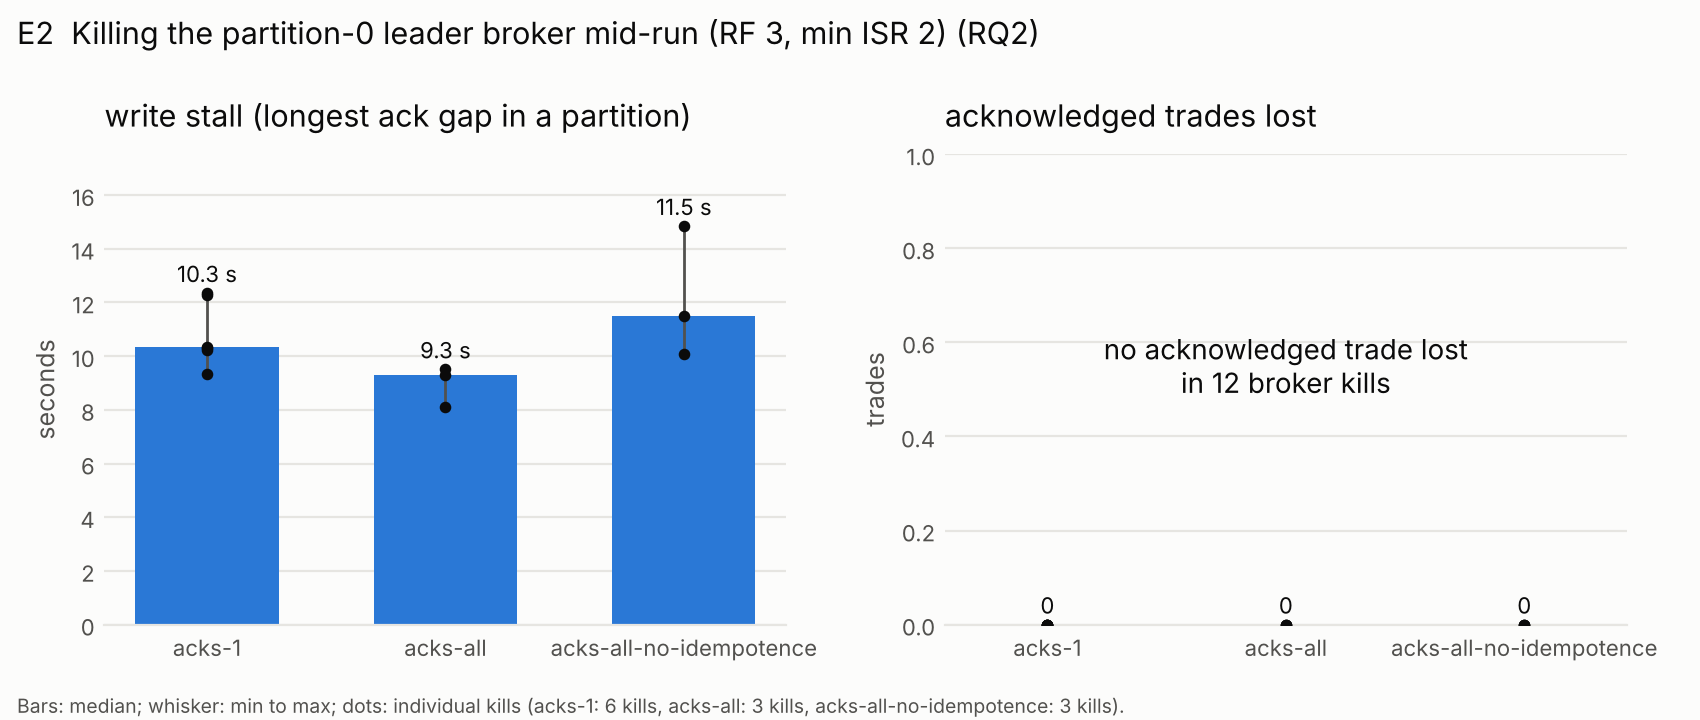
\includegraphics[width=0.9\textwidth]{e2_broker_crash.png}
\caption{E2: write stall and lost trades after a leader kill.}
\label{fig:e2}
\end{figure}

\subsection{E3: Spark crash (RQ2)}
We sent SIGKILL to the Spark container and restarted it at once on the same checkpoint. The first new bar
appeared 12.8 s [12.6 to 12.9] later in deterministic replay and 14.6 s [14.2 to 14.9] later on a live
stream, and the output was exact in all six runs. Almost all of that time is JVM and Spark start-up:
the first completed batch came 12.8 to 13.4 s after the restart. See Figure~\ref{fig:e3}.

\begin{figure}[H]
\centering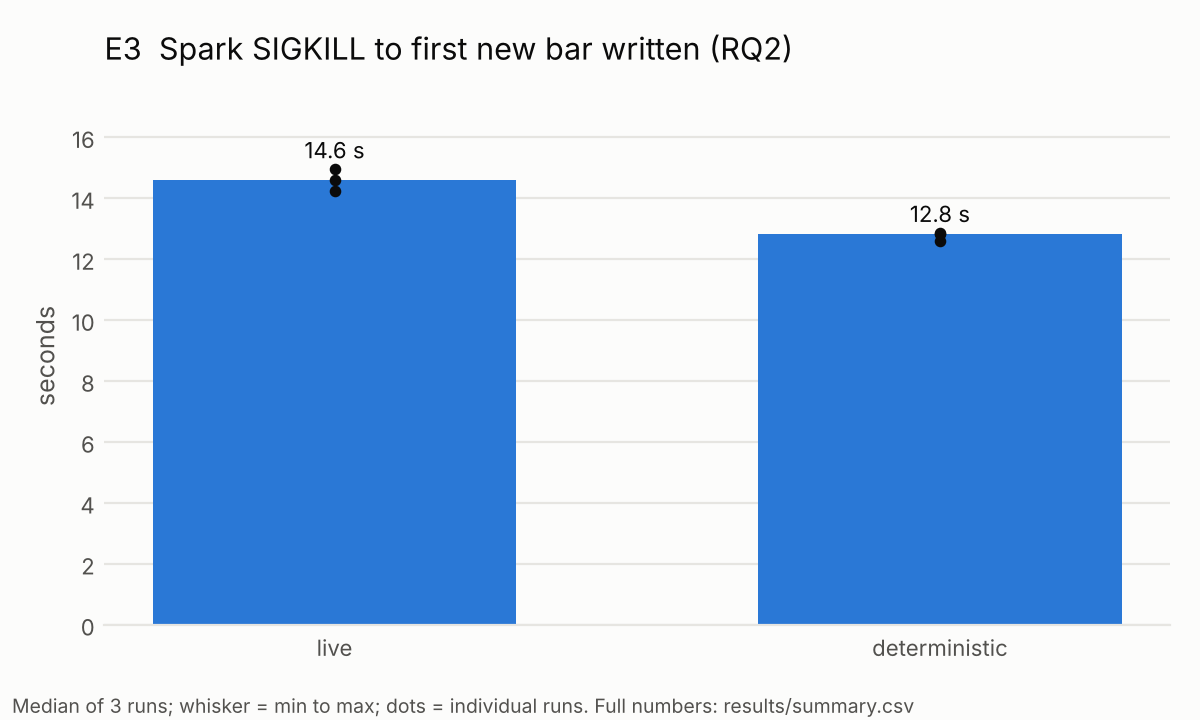
\includegraphics[width=0.7\textwidth]{e3_spark_recovery.png}
\caption{E3: time from the kill to the first new bar.}
\label{fig:e3}
\end{figure}

\subsection{E4: cost of exactly-once output (RQ3)}
We made Spark kill itself after the database commit and before Spark recorded the batch, so the restart
replays a batch that is already in the database. With plain inserts this left 300 duplicate bar rows in every
run, and with upserts none (three runs each). Without a crash, at 2,000 records per second, we could
not measure a cost for upserting. Batch duration p50 was 460 ms for inserts and 451 ms for upserts. Bar
latency p50 was 1.7 s [1.5 to 1.9] against 2.1 s [1.7 to 2.3], with overlapping ranges, and p99 was
2.45 s against 2.43 s. Both kept up. Figure~\ref{fig:e4} shows the results.

\begin{figure}[H]
\centering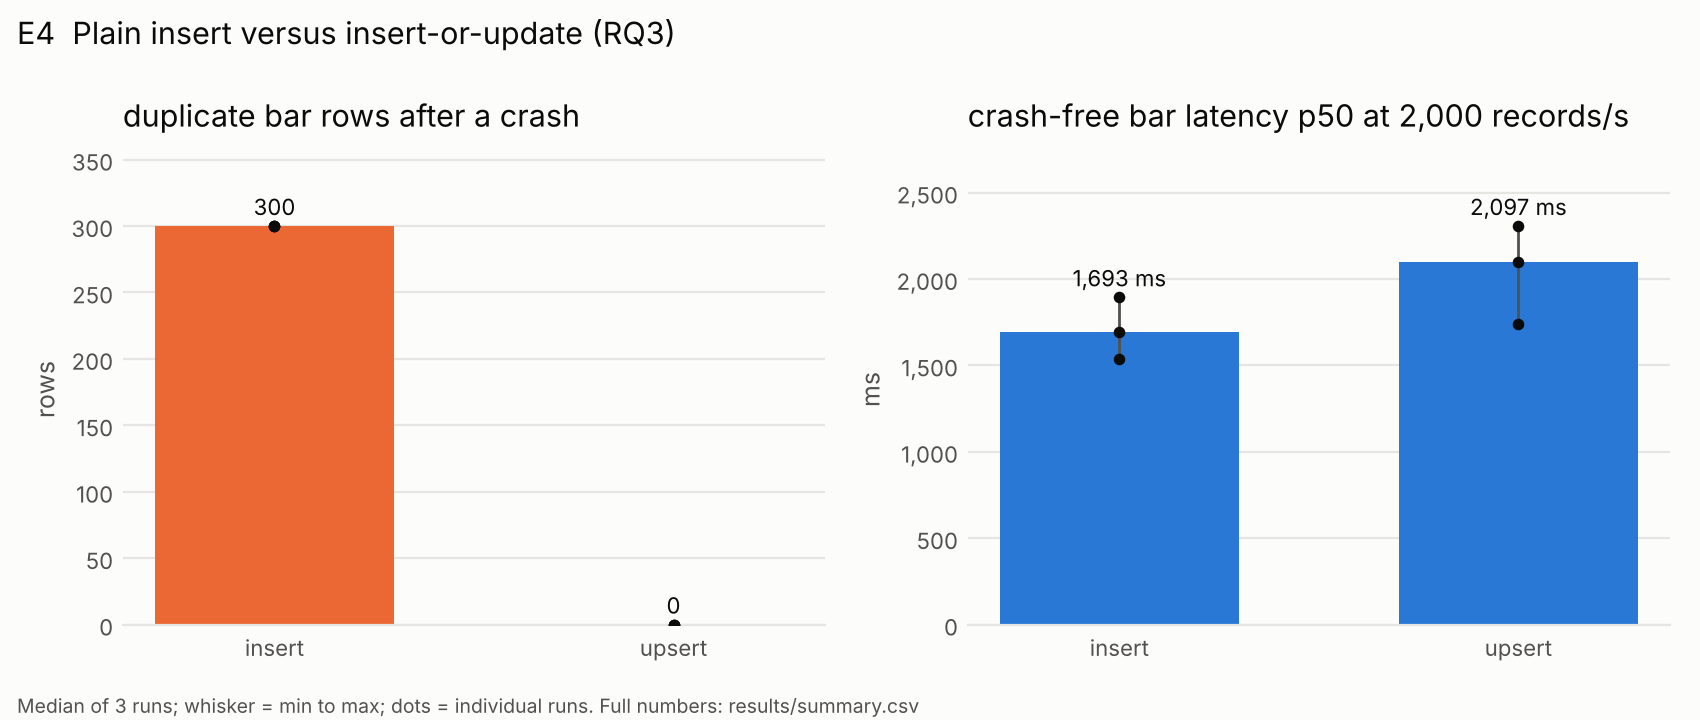
\includegraphics[width=0.9\textwidth]{e4_exactly_once.png}
\caption{E4: duplicate rows after a crash, and the cost of upserts without one.}
\label{fig:e4}
\end{figure}

\subsection{Live Coinbase run}
\label{sec:live}
We also ran the pipeline on live trades from Coinbase's public market-data feed for ten products (BTC, ETH,
SOL, XRP, DOGE, ADA, AVAX, LINK, LTC and BCH), on a Windows laptop with Docker Desktop, for more than 20
minutes. The producer connected to the feed, sent every trade to Kafka with acks=all, and saved a capture. The
dashboard filled with one-minute bars for all ten symbols, with Spark's lag at zero. No alert fired, which is
expected: live prices rarely move three standard deviations from their previous 30 one-minute returns, while the
synthetic data injects such shocks on purpose. After stopping the producer we ran the verifier against the
topic's own contents, because no generator file exists for live data. All 230 bars matched exactly (none
missing, extra, duplicated or different), and there were no alerts to match.

%------------------------------------------------------------------------------------------------
\section{Discussion: reproduction and extension}
\paragraph{Reproduction (a).} Batching raises producer throughput by more than an order of magnitude,
as Kreps et al.\ found, so the shape holds. Our unbatched rate is lower than theirs because every
one-record request is a round trip on a single shared four-core machine, and our batched rates are
higher because the producer and the CPU are newer. The paper used two dedicated 8-core machines, and we
approximate a batch of $n$ messages as $n \times 200$ bytes, since the Java producer sizes batches in bytes.

\paragraph{Reproduction (b).} Continuous processing gives much lower latency (tens of milliseconds
against hundreds) up to a saturation point, past which its latency climbs steeply, while micro-batch
sustains a higher input rate. The shape matches Armbrust et al. Their continuous latency was about
1 ms, and ours is tens of milliseconds because ours includes the producer's batching (\code{linger.ms}
of 5), a Kafka write with acks=all on three replicas, and the sink's own producer. The limit of one
core per partition on four cores is the constraint the paper describes, and we hit it.

\paragraph{Extension.} For RQ2, with replication factor 3 and a minimum ISR of 2, no acknowledged trade
was lost in 12 leader kills. The price of acks=all is a stall of about 9 s on every partition until the
dead broker is fenced. Acks=1 confines the stall to the dead broker's partitions but can lose
acknowledged writes, which we saw once, in a dry run. Spark recovers from its own crash in 13 to 15 s
with exact output. For RQ3, plain inserts are wrong after a crash (300 duplicate rows every time), and upserts
are exact at no cost we could measure at 2,000 records per second.

%------------------------------------------------------------------------------------------------
\section{Challenges}
\label{sec:challenges}
\begin{enumerate}
  \item \textbf{Determinism against late data.} An unpaced replay squeezes 40 virtual minutes into a few
        seconds, so a few milliseconds of skew between partitions looked like more than the 10 s watermark
        and trades would have been dropped as late. We now preload the topic before Spark starts.
  \item \textbf{Duplicates from producer retries.} With acks=all but idempotence off, killing a leader made
        the producer write one trade twice, and the verifier caught the wrong bar. Idempotence is now the
        default, and E2 measures the difference.
  \item \textbf{Measuring a write stall.} Looking at all partitions together hid the acks=1 behavior.
        We now compute the stall per partition from timestamped acknowledgements.
  \item \textbf{JVM warm-up} made the first latencies about twenty times worse, so we discard a warm-up
        period.
  \item \textbf{Continuous mode needs a core per partition.} With 6 partitions on 4 cores, two partitions were
        never processed, with no error. Continuous runs use 4 partitions.
  \item \textbf{Crashing between two commits.} A SIGKILL sent to PID 1 inside a container is ignored. The fault
        hook needed an init process and a kill of the driver JVM from inside \code{foreachBatch}.
  \item \textbf{Floating-point equality.} Fractional crypto sizes summed in a different order differ in
        the last bits, so the verifier allows a relative $10^{-9}$ for volume only.
  \item \textbf{Versions and tooling.} We checked that Kafka 4.4, Spark 4.2, PostgreSQL 18 and Grafana 13
        exist before pinning them, and had to build images behind a TLS-inspecting proxy and around Docker
        Hub rate limits.
  \item \textbf{Live data access.} The cloud development environment could not reach the Coinbase feed, so we
        first tested the adapter against a fake server that follows the protocol, and from captured sessions. We
        later ran it on a laptop (Section~\ref{sec:live}). Getting the stack to start on Windows took four fixes
        (a Linux-only default path, a missing image build, and two host ports that Windows had reserved or
        another project was using).
\end{enumerate}

%------------------------------------------------------------------------------------------------
\section{Reproducibility}
\label{sec:repro}
The repository holds everything needed to repeat the work. \code{docker compose up} starts the pipeline
and the demo. Image tags and Python packages are pinned and locked. A golden dataset with a SHA-256
manifest lets \code{make golden} replay a known stream through Kafka and Spark and check every bar and
alert against the oracle. \code{make bench-all} runs every experiment (about 12 hours), and
\code{uv run python -m bench.summarize} rebuilds every table and figure from the raw runs. Each run stores
its parameters, versions, git commit and machine. Continuous integration runs the linter, the unit tests and
the PostgreSQL integration tests on every push. The README explains how to run each step.

%------------------------------------------------------------------------------------------------
\section{Limitations: what one machine can and cannot show}
\label{sec:limits}
All three brokers, Spark (\code{local[4]}), PostgreSQL, Grafana, the generator and the measuring harness
ran on one virtual machine with 4 CPUs and 16 GB. Every container shares those four cores, one disk and
the loopback network. Our results are therefore sound for what they compare on this machine and weak as
absolute numbers.

\subsection{Throughput}
\begin{itemize}
  \item \textbf{Components compete for the same CPUs.} A measured rate is the pipeline's capacity while the
        generator, three brokers and PostgreSQL also run. On a cluster Kafka, Spark and the producers would
        have their own cores and every rate here would probably be higher. We report sustained rates as
        properties of this machine, not as limits of Kafka or Spark.
  \item \textbf{Our input is itself a ceiling.} The Python generator tops out near 100,000 records per second
        while Spark runs beside it. ``At least 90,000'' and ``micro-batch kept up at 100,000'' mean that the
        pipeline did not saturate before our input did. The true maximum is unknown.
  \item \textbf{Partition scaling is capped by cores.} More partitions than cores did not help (E1b, E1c). That
        shows the four-core limit and says nothing about how Kafka scales. The benefits of partitions in
        production, such as consumers on many machines and many disks, cannot appear here.
  \item \textbf{No network cost.} Replication between brokers crosses the loopback interface, so the latency of
        acks=all, which waits for replicas over a real network, is understated. E1a also differs from the
        paper because producer and broker share cores, where the paper used two 8-core machines.
  \item \textbf{One disk and the page cache.} Kafka depends on sequential disk writes and the page cache.
        Three brokers on one volume cannot show per-broker disk limits, and we did not enable \code{fsync}.
  \item \textbf{Changing hardware.} The virtual machine's CPU changed from 2.30 to 2.10 GHz between two
        experiments. We added a baseline setting (\code{p6-1s-b}) and compare triggers only within one machine
        state. Three runs per setting give a range, not a confidence interval.
  \item \textbf{Synthetic data.} Every measurement uses the seeded generator. Live Coinbase data appears only
        in the demonstration and in the short run of Section~\ref{sec:live}.
\end{itemize}

\subsection{Fault tolerance}
\begin{itemize}
  \item \textbf{A killed container is not a failed node.} \code{docker kill} stops one broker process at once.
        It does not model a network partition, a slow or full disk, a failed rack, a lost machine, or two
        brokers failing together. With three brokers on one host, the host is a single point of failure that
        none of our experiments can survive.
  \item \textbf{Detection time is configuration, not network behavior.} The 9 s stall in E2 equals the
        controller's \code{broker.session.timeout.ms} of 9,000 ms. On a real network, detection also depends on
        latency, partitions and clocks, and the stall could be shorter if tuned, or longer. We measured how this
        configuration reacts to a clean kill, not how fast Kafka recovers in general.
  \item \textbf{We injected the favorable failure.} A crashed leader's followers hold identical data, so a
        minimum ISR of 2 with unclean election off loses nothing. A leader that stays up but is cut off from
        its followers would test those settings harder, and we cannot produce that here.
  \item \textbf{Spark recovery excludes a cluster.} \code{local[4]} has no executors to lose, no rescheduling and
        no network shuffle. E3 measures checkpoint recovery of the driver (JVM start, state restore and
        replay), which is real, but not recovery on a standalone, YARN or Kubernetes cluster.
  \item \textbf{Time compression magnifies skew.} The crash experiments run virtual time ten times faster than
        the wall clock. A failover skew of a few seconds between partitions became tens of seconds of event
        time and made the 10 s watermark drop trades in one run (Section~\ref{sec:results}). With real-time data
        the same skew is ten times smaller relative to the watermark, so the failure would be rarer. The
        lesson that the watermark must exceed the partition skew still holds.
  \item \textbf{One local database.} A single PostgreSQL on the same machine has no network round trip and no
        competing writers, so the upsert cost we measured at 2,000 records per second is a lower bound for a
        remote or shared database.
\end{itemize}

\subsection{What still holds}
The correctness results do not depend on the machine. The bars and alerts match the oracle in every run,
no acknowledged trade was lost, and the duplicate rows in E4 follow from the protocol: a crash between
the database commit and Spark's commit replays the batch. The relative comparisons made on one machine
state (batching against none, continuous against micro-batch, trigger intervals, insert against upsert)
are valid for that machine, and their shapes agree with the published papers. We described Kafka's
security features (TLS, SASL, ACLs) but did not measure them. The harness could be pointed at a
multi-node cluster to extend the study.

%------------------------------------------------------------------------------------------------
\section{Conclusion}
\paragraph{RQ1.} The processing mode sets the latency floor. Continuous processing answers in tens of
milliseconds but saturates between 40,000 and 80,000 records per second on four cores, while micro-batch
trades hundreds of milliseconds for at least 100,000 records per second. For the bars pipeline the
trigger should match the load: 500 ms at moderate load, 1 s at high load, and 5 s was never best. More
partitions than cores did not help.

\paragraph{RQ2.} With replication factor 3 and a minimum ISR of 2, no acknowledged trade was lost in 12
leader kills. Acks=all stalls all writes for about 9 s until the dead broker is fenced, and acks=1 stalls
only its partitions but can lose acknowledged writes. A failover can also make Spark drop trades as late
when the watermark is shorter than the skew between partitions. Spark recovers from its own crash in
about 13 to 15 s with exact output.

\paragraph{RQ3.} Exactly-once output needs an idempotent sink. Plain inserts duplicated 300 rows after
every crash between the database commit and Spark's commit, upserts duplicated none, and at 2,000 records
per second the upsert cost nothing measurable.

\bibliographystyle{unsrt}
\bibliography{references}

%------------------------------------------------------------------------------------------------
\appendix
\section{Configuration of each experiment}
\label{app:config}
These tables come from \path{docker-compose.yml}, the topic script, the generator's defaults and the
experiment definitions in \path{bench/experiments/}. Each run also stores its own parameters in
\path{config.json} next to its raw output.

\subsection{Settings shared by all experiments}
\begin{table}[H]
\centering\small
\caption{Stack settings.}
\begin{tabularx}{\textwidth}{@{}>{\raggedright\arraybackslash}p{3.2cm}Y@{}}
\toprule
Component & Setting \\
\midrule
Kafka brokers & Image \code{apache/kafka:4.4.0}; 3 nodes, each broker and controller (KRaft combined mode); heap 1 GB per broker; \code{default.replication.factor=3}; \code{min.insync.replicas=2}; \code{unclean.leader.election.enable=false}; \code{auto.create.topics.enable=false}; PLAINTEXT listeners; no \code{log.flush.*} override; failure detection at the defaults (session timeout 9,000 ms, heartbeat 2,000 ms). \\
Topics & \code{trades}: 6 partitions by default (set per experiment), RF 3, min ISR 2, retention 1 day. \code{passthrough\_out}: same partitions as \code{trades}, RF 3, min ISR 2, \code{LogAppendTime}, retention 1 day. \code{perf\_test}: 1 partition, RF 1, min ISR 1, retention 1 hour. \\
Spark & Image \code{spark:4.2.1-scala2.13-java17-python3-ubuntu} with the Kafka connector \code{spark-sql-kafka-0-10\_2.13:4.2.1}; \code{--master local[4]}; driver memory 2 GB; container limit 4 CPUs and 3 GB; \code{spark.sql.shuffle.partitions=4}; session time zone UTC; \code{failOnDataLoss=true}; checkpoints on a named volume. \\
Bars job & Trigger 1 s; watermark 10 s; sink mode upsert; \code{startingOffsets=earliest}. \\
Pass-through job & Micro-batch trigger 100 ms, or continuous with a 1 s checkpoint interval; \code{startingOffsets=latest}. \\
PostgreSQL & Image \code{postgres:18.6}. \\
Producer (\code{confluent-kafka}) & \code{linger.ms=5}; \code{batch.size=1000000}; \code{retries=2147483647}; \code{queue.buffering.max.messages=500000}; \code{acks=all} with \code{enable.idempotence=true}, except where an experiment says otherwise (idempotence cannot be combined with acks=1). \\
\bottomrule
\end{tabularx}
\end{table}

\subsection{Settings per experiment}
\begin{table}[H]
\centering\footnotesize
\caption{Per-experiment settings. ``Records/s'' is the input rate.}
\begin{tabularx}{\textwidth}{@{}>{\raggedright\arraybackslash}p{1.1cm}YYY@{}}
\toprule
 & Kafka & Spark & Producer and input \\
\midrule
E1a & \code{perf\_test}: 1 partition, RF 1, min ISR 1; topic recreated for each setting & None & \code{kafka-producer-perf-test} inside \code{kafka-1}, 10 million records of 200 bytes, unlimited rate, \code{acks=0}; \code{batch.size} 0, 2,000, 10,000, 20,000, 40,000 bytes; \code{linger.ms} 0 (batch 1) or 10 \\
E1b & \code{trades} and \code{passthrough\_out}: 4 partitions, RF 3, min ISR 2 & Pass-through job; continuous (1 s checkpoint) or micro-batch (100 ms trigger); \code{startingOffsets=latest} & Realtime, \code{acks=all}, idempotent; continuous at 5,000, 10,000, 20,000, 40,000 and 80,000 records/s for 120 s (20 s warm-up); micro-batch at 40,000, 80,000 and 100,000 for 300 s (30 s warm-up) \\
E1c & \code{trades}: 1, 3 or 6 partitions, RF 3, min ISR 2; recreated before each step & Bars job, upsert sink; trigger 100 ms, 500 ms, 1 s or 5 s; \code{startingOffsets=latest} & Realtime, \code{acks=all}, idempotent, no closing trade; 30,000, 60,000 and 90,000 records/s, 300 s per step, 70 s warm-up; settings p1, p3, p6 with a 1 s trigger, and p6 with 100 ms, 500 ms, 5 s, plus a repeat of p6 at 1 s \\
E2 & \code{trades}: 6 partitions, RF 3, min ISR 2; the leader of partition 0 killed at 50\% of the run & Bars job, trigger 1 s, \code{startingOffsets=earliest} & Virtual mode, seed 42, 40 virtual minutes at 10 times speed, 1.0 trades per symbol per virtual second; acks=all with idempotence (3 kills), acks=1 (6 kills), acks=all without idempotence (3 kills) \\
E3 & \code{trades}: 6 partitions, RF 3, min ISR 2 & Bars job; SIGKILL at 50\% of the stream (live) or after batch 5 (deterministic, \code{maxOffsetsPerTrigger=5000}); restart at once on the same checkpoint & Live: virtual mode, seed 42, 40 minutes at 10 times speed. Deterministic: golden dataset (60,163 trades) preloaded and replayed at maximum speed. \code{acks=all}, idempotent \\
E4 & \code{trades}: 6 partitions, RF 3, min ISR 2 & Bars job; sink insert (\code{bars\_plain}) or upsert (\code{bars}); crash runs use \code{FAULT\_AFTER\_BATCH=5} and \code{maxOffsetsPerTrigger=5000} & Crash runs: golden replay. Cost runs: realtime at 2,000 records/s for 300 s, 70 s warm-up, no crash \\
\bottomrule
\end{tabularx}
\end{table}

\section{Machine and versions}
\label{app:machine}
Runs started on 11 November 2026 and finished on 12 November 2026 (72 runs, none failed). The development
virtual machine was moved between physical hosts when it restarted, so two CPUs appear. Both are 4-vCPU Intel
Xeon virtual machines with 15.7 GB of memory, Docker 29.9.2 and Linux 6.18.44: machine A at 2.10 GHz and
machine B at 2.30 GHz. Table~\ref{tab:machines} says which experiments ran where, and results are compared
only within one machine.

\begin{table}[H]
\centering\small
\caption{Where each experiment ran.}
\label{tab:machines}
\begin{tabular}{@{}ll@{}}
\toprule
Machine & Settings \\
\midrule
A (2.10 GHz) & E1c p6-100ms, p6-500ms, p6-5s and p6-1s-b; E2 (all); E3 (all); E4 crash runs \\
B (2.30 GHz) & E1a (all); E1b (all); E1c p1-1s, p3-1s and p6-1s; E4 cost runs \\
\bottomrule
\end{tabular}
\end{table}

\noindent Software: Apache Kafka 4.4.0, Apache Spark 4.2.1 (PySpark, Python 3.10 in the image), PostgreSQL
18.6, Grafana 13.3.0; on the host Python 3.13, confluent-kafka 2.16.1, psycopg 3.3.8, numpy 2.5.3 and
pandas 3.0.5, all pinned in the repository's lock file.

%   3. Add the packages below to the template's preamble if it does not load them already:
%        booktabs, tabularx, array, graphicx, float, caption, enumitem, tikz (with libraries
%        positioning, arrows.meta, shapes.geometric, fit, backgrounds), xurl, hyperref
%        and this macro:   \newcommand{\code}[1]{\texttt{#1}}
%        and this column type:   \newcolumntype{Y}{>{\raggedright\arraybackslash}X}
%        and:   \graphicspath{{figures/}}
%   4. If the template sets up its own bibliography, delete the two lines near the end of this file
%      (\bibliographystyle and \bibliography) and keep the template's.
%
% report/main.tex is a ready-made wrapper that does exactly this, so it compiles on its own.

\begin{abstract}
Trading desks want per-minute summaries and alerts within seconds of each trade. We built that
pipeline from Apache Kafka 4.4 (three brokers, KRaft) and Spark 4.2 Structured Streaming (PySpark).
It writes one-minute open, high, low, close and volume-weighted average price (VWAP) bars and
three-sigma alerts to PostgreSQL, shows them in Grafana, and starts with one \code{docker compose up}.
A seeded generator makes the correct output known exactly, so we check every run bar by bar. We
reproduce two published results, producer batching (Kreps et al., Figure 4) and continuous versus
micro-batch latency (Armbrust et al., Figure 7), and add what neither paper measured: whether the output
stays correct when a broker or the Spark job crashes, and what exactly-once output costs. No
acknowledged trade was lost in 12 broker crashes. Spark recovered from its own crash in about 14
seconds with exact output. Plain inserts left 300 duplicate rows after every crash, while upserts left
none and cost nothing we could measure at 2,000 trades per second. All measurements come from one
4-CPU machine, and Section~\ref{sec:limits} says what that does to the conclusions.
\end{abstract}

%------------------------------------------------------------------------------------------------
\section{Background and significance}
Market data arrives as a continuous stream of trades. A common design pairs a durable, partitioned
log that stores the events with a stream processor that reads the log and computes results over time
windows.

\paragraph{Apache Kafka.} Kafka~\cite{kreps2011,wang2015} is the log. A topic is split into
partitions, and each partition is an append-only file on a broker, written and read sequentially in
batches. Kreps et al.\ showed that this gives much higher throughput than traditional message
queues~\cite{kreps2011}. Kafka orders events only within a partition, so keying trades by symbol keeps
each symbol's trades in order. Each partition is copied to several brokers: a leader serves reads and
writes, and the followers that are caught up form the in-sync replica set (ISR). Whether an acknowledged
write survives a broker crash depends on three settings: the replication factor, the number of copies
the producer waits for (\code{acks}), and the minimum number of in-sync replicas~\cite{wang2015}. Kafka 4
keeps cluster metadata in its own Raft-based protocol (KRaft), so it no longer needs ZooKeeper.

\paragraph{Spark Structured Streaming.} Structured Streaming~\cite{armbrust2018} is the processor. It
treats a stream as an unbounded table and runs a normal SQL-style query over it incrementally, usually
in micro-batches, an approach that descends from discretized streams~\cite{zaharia2013}. It aggregates
over event-time windows and keeps intermediate state between batches. A watermark says how long Spark
waits for late events before it finalizes a window, an idea from the Dataflow model~\cite{akidau2015}.
Spark records each batch's Kafka offsets and its state in a checkpoint. Kafka can re-deliver from any
offset, so after a crash Spark re-runs exactly the unfinished batches, and an idempotent sink then makes
the result the same as if each event had been processed once. An experimental continuous mode lowers
latency, but it supports only per-record operations and delivers at least once.

\paragraph{Why test them together.} The papers promise high throughput from batched sequential I/O,
durability from replication, and exactly-once results from replay plus checkpoints. Each promise
depends on configuration and on how the two systems are connected. We test them on a financial
workload with a known correct answer, and we focus on the seam between the systems more than on either
one alone.

%------------------------------------------------------------------------------------------------
\section{Goals and objectives}
We set out to answer three research questions.
\begin{enumerate}[label=\textbf{RQ\arabic*.},leftmargin=*]
  \item How do the number of partitions, the trigger interval and the processing mode trade latency
        against throughput?
  \item Which Kafka settings prevent lost or duplicated data when a broker crashes, and how long does
        Spark take to recover from its own crash?
  \item What does exactly-once output cost compared with at-least-once output?
\end{enumerate}
The objectives are: (1) explain how Kafka, Spark and their integration work; (2) build a case-study
pipeline that starts with one command; (3) reproduce Kreps et al.\ Figure~4 and Armbrust et al.\
Figure~7, comparing the shape of each curve and not the absolute numbers; (4) extend both papers with
experiments they did not run, namely correctness under crashes and the cost of exactly-once output;
and (5) publish a repository that others can run, with pinned versions and scripted experiments.

%------------------------------------------------------------------------------------------------
\section{Architecture analysis}
\label{sec:arch}
Figure~\ref{fig:pipeline} shows the pipeline we built. A generator publishes trades, keyed by symbol,
to a topic with six partitions. Spark reads one task per partition, builds one-minute bars with a
10-second watermark, and writes each batch to PostgreSQL in one transaction. Grafana reads PostgreSQL.

\begin{figure}[H]
\centering
\resizebox{\textwidth}{!}{%
\begin{tikzpicture}[
  node distance=9mm and 8mm,
  box/.style={draw,rounded corners=2pt,align=center,inner sep=4pt,font=\small,minimum height=10mm},
  store/.style={draw,cylinder,shape border rotate=90,aspect=0.25,align=center,font=\small,minimum height=11mm,inner sep=3pt},
  arr/.style={-{Stealth[length=2mm]},thick},
  lab/.style={font=\scriptsize,align=center}]
  \node[box] (gen) {Generator\\(seeded, or\\Coinbase live)};
  \node[box,right=26mm of gen] (kafka) {Kafka, 3 brokers\\topic \code{trades}\\6 partitions, RF 3,\\min ISR 2};
  \node[box,right=26mm of kafka] (spark) {Spark\\\code{local[4]}, 1 s trigger\\watermark 10 s,\\1-minute windows};
  \node[store,right=30mm of spark] (pg) {PostgreSQL\\bars, alerts};
  \node[box,right=12mm of pg] (graf) {Grafana};
  \node[store,below=8mm of spark] (ck) {Checkpoint\\volume};
  \draw[arr] (gen) -- node[lab,above]{key = symbol} node[lab,below]{acks=all} (kafka);
  \draw[arr] (kafka) -- node[lab,above]{one task per} node[lab,below]{partition} (spark);
  \draw[arr] (spark) -- node[lab,above]{one transaction} node[lab,below]{per batch} (pg);
  \draw[arr] (pg) -- (graf);
  \draw[arr,dashed] (spark) -- node[lab,right]{offsets, state} (ck);
\end{tikzpicture}}
\caption{The pipeline. A separate pass-through job (not shown) copies \code{trades} to a second
topic for the latency experiments.}
\label{fig:pipeline}
\end{figure}

\subsection{Kafka}
Table~\ref{tab:kafka} lists the Kafka mechanisms we rely on and where each one shows up in the project.

\begin{table}[H]
\centering\small
\caption{Kafka mechanisms and their role in this project.}
\label{tab:kafka}
\begin{tabularx}{\textwidth}{@{}>{\raggedright\arraybackslash}p{3.1cm}YY@{}}
\toprule
Mechanism & How it works & In this project \\
\midrule
Partitions and ordering & A partition is an append-only log on a broker, written and read sequentially. Order holds only within a partition; the producer picks the partition by hashing the key. & \code{trades} has 6 partitions on 3 brokers. Key = symbol, so every symbol lands in one partition and stays in order (checked from the acknowledgement log). \\
Throughput design~\cite{kreps2011} & Batching many records per request, sequential disk I/O, the page cache, zero-copy transfer. & E1a reproduces the batching effect. \\
Retention & Records stay for a time or size limit whether or not they were read, so a consumer can re-read from any offset. & \code{trades} keeps one day. Replay after a crash depends on it. \\
Replication and ISR~\cite{wang2015} & A partition has a leader and followers. A write is committed when every in-sync replica has it. & RF 3, \code{min.insync.replicas=2}, unclean leader election off, so only an in-sync replica can become leader. \\
Producer \code{acks} & 0: no wait. 1: the leader only. all: every in-sync replica. & E2 kills a leader with acks=1 and acks=all. \\
Idempotent producer & The broker drops a retried batch it has already seen, using the producer id and a sequence number. & On by default with acks=all. Without it, a leader kill once duplicated a trade (Section~\ref{sec:challenges}). \\
KRaft & Metadata lives in a Raft-replicated log on controller nodes. & Three nodes, each broker and controller. \\
Consumer groups & Consumers with one \code{group.id} split a topic's partitions, and Kafka stores the group's committed offsets. & Used by our verifier and latency collectors. Spark does not use them (Section~\ref{sec:integration}). \\
Delivery guarantees & At most once, at least once, or exactly once (idempotent producer plus transactions inside Kafka). & End-to-end exactly-once here comes from Spark's replay plus an idempotent sink. \\
Security & TLS encrypts traffic, SASL authenticates clients, ACLs authorize operations. & Described, not measured. The stack runs PLAINTEXT on one machine, with Grafana and PostgreSQL bound to localhost. \\
\bottomrule
\end{tabularx}
\end{table}

\subsection{Spark Structured Streaming}
Table~\ref{tab:spark} does the same for Spark.

\begin{table}[H]
\centering\small
\caption{Spark mechanisms and their role in this project.}
\label{tab:spark}
\begin{tabularx}{\textwidth}{@{}>{\raggedright\arraybackslash}p{3.1cm}YY@{}}
\toprule
Mechanism & How it works & In this project \\
\midrule
Unbounded table~\cite{armbrust2018} & A streaming query is an ordinary DataFrame query that Spark runs incrementally. The optimizer turns it into an incremental plan with stateful operators. & The bars job is a \code{groupBy(window, symbol)} aggregation. \\
Micro-batch and triggers~\cite{zaharia2013} & A trigger starts a batch at fixed intervals; each batch reads the offsets that arrived since the last one. & Trigger 1 s by default. E1c varies it from 100 ms to 5 s. \\
Continuous processing & Long-running tasks handle one record at a time and checkpoint in epochs. Lower latency, but only map-like operations, at-least-once, and one core per input partition. & Cannot run the bars job. E1b runs a pass-through job in both modes. With 6 partitions on 4 cores, two partitions were never processed. \\
Event time and watermark~\cite{akidau2015} & Windows follow the record's event time. The watermark is the largest event time seen minus a delay. In append mode a window is emitted once, when the watermark passes its end. & One-minute tumbling windows, 10 s watermark. A closing trade for a reserved symbol advances the watermark past the last windows. \\
State store & Partial aggregates per window and key, written to the checkpoint every batch and dropped after the watermark passes. & Open, high, low, close (using \code{min\_by} and \code{max\_by} on time and trade id), volume, notional, count. \\
Checkpoint & \code{offsets/} (the range each batch will read, written before processing), \code{commits/} (finished batches), \code{state/}. & A named volume that survives \code{docker kill}. E3 and E4 depend on it. \\
Sinks & Append, update or complete output; \code{foreachBatch} hands each batch to user code; the Kafka sink is at least once. & Append mode with \code{foreachBatch} into PostgreSQL. The pass-through job uses the Kafka sink. \\
Monitoring & A \code{StreamingQueryListener} receives one progress event per batch. & Written to a \code{query\_progress} table that feeds the dashboard and the throughput tests. \\
\bottomrule
\end{tabularx}
\end{table}

\subsection{Integration}
\label{sec:integration}
\paragraph{Partitions become tasks.} The Kafka source plans one Spark task per Kafka partition in each
batch, so the partition count bounds parallelism. E1c compares 1, 3 and 6 partitions on 4 cores.

\paragraph{Offsets live in Spark's checkpoint, not in a consumer group.} Spark picks each batch's offset
range and writes it to the checkpoint before it processes anything. That ties the offsets to the batch
id and to a version of the state. A consumer group's committed offset cannot do that: it says
``consumed'', not ``consumed and reflected in state version $n$ and in output batch $n$''. After a
crash Spark reads exactly the uncommitted range again. This requires Kafka to still hold the data
(\code{failOnDataLoss=true} stops the query if it does not) and the checkpoint to match the topic, so our
harness always wipes both together.

\paragraph{Exactly-once output is replay plus an idempotent sink.} Replay delivers a crashed batch a
second time, and the sink must make the second write harmless. Each batch's bars and alerts go to
PostgreSQL in one transaction, using \code{INSERT ... ON CONFLICT (symbol, window\_start) DO UPDATE},
and the \code{written\_at} column is set only on the first insert. Figure~\ref{fig:batch} shows the order
of events in one batch. A crash anywhere before the commit record makes Spark run the batch again from
the same offsets, and the upsert absorbs it. E4 tests exactly that.

\begin{figure}[H]
\centering\small
\begin{tabularx}{\textwidth}{@{}rlY@{}}
\toprule
Step & Actor & Action \\
\midrule
1 & Spark driver & Ask Kafka for the latest offset of every partition. \\
2 & Spark driver & Write the planned offset range to the checkpoint (\code{offsets/n}). \\
3 & Spark tasks & Read that range, one task per partition, and update the aggregation state. \\
4 & Spark driver & Emit the windows the watermark has passed. \\
5 & Sink & In one transaction: upsert the bars, read the 31 previous bars of each symbol, upsert the alerts, commit. \\
6 & Spark driver & Write \code{commits/n} and state version $n$. \\
\bottomrule
\end{tabularx}
\caption{One micro-batch. A crash between steps 5 and 6 replays the batch.}
\label{fig:batch}
\end{figure}

\subsection{Failure behavior}
Table~\ref{tab:failure} lists each failure we injected or considered and what the experiments showed.

\begin{table}[H]
\centering\small
\caption{Failure behavior and where we measured it.}
\label{tab:failure}
\begin{tabularx}{\textwidth}{@{}>{\raggedright\arraybackslash}p{3.6cm}Yl@{}}
\toprule
Failure & What happens & Measured in \\
\midrule
Leader broker killed, acks=all & Writes to every partition stall until the controller fences the dead broker and removes it from the ISR; then they continue. No acknowledged trade is lost. The stall matches \code{broker.session.timeout.ms} (9,000 ms) plus up to one heartbeat interval. & E2 \\
Leader broker killed, acks=1 & Only the partitions the dead broker led stall. Records it had acknowledged but not yet replicated can be lost when a follower takes over; not every kill loses data. & E2 \\
Producer retry without idempotence & A retried batch can be written twice. & E2, Section~\ref{sec:challenges} \\
Spark killed & Spark restarts from the checkpoint. Recovery time is mostly JVM and Spark start-up. Output stays exact with the upsert sink. & E3 \\
Spark killed after the sink commits & Spark replays the batch: duplicates with plain inserts, none with upserts. & E4 \\
Topic recreated under a checkpoint & \code{failOnDataLoss=true} stops the query instead of skipping data. & Harness procedure \\
\bottomrule
\end{tabularx}
\end{table}

\subsection{Design choices}
Several choices trade one property for another. A shorter watermark lowers bar latency but drops more
late trades, and because we measure latency from the window end plus the watermark, the watermark
adds directly to the time to result. A shorter trigger lowers latency but adds per-batch overhead
(E1c). More partitions add parallel tasks but also state-store and planning work on four cores. Setting
acks=all with a minimum ISR of 2 survives one broker failure at the price of a write stall while the
ISR shrinks (E2). We read the alert history back from PostgreSQL, which keeps the Spark job a plain
windowed aggregation, at the cost of one indexed query per batch. Running Spark as \code{local[4]} in one
container matches the 4-core setup of Armbrust et al.\ and our memory budget, but it is not a test of
distributed Spark.

%------------------------------------------------------------------------------------------------
\section{Features exercised}
\begin{table}[H]
\centering\small
\caption{Each feature, how the pipeline uses it, and what demonstrates it.}
\begin{tabularx}{\textwidth}{@{}>{\raggedright\arraybackslash}p{3.4cm}YY@{}}
\toprule
Feature & Use in the pipeline & Demonstrated by \\
\midrule
Partitioned, keyed log & 6 partitions, key = symbol, per-symbol order & Acknowledgement-log check; E1c \\
Replication and acks & RF 3, min ISR 2, acks=all, idempotent producer & E2 \\
Event-time windows and watermark & 1-minute bars, 10 s watermark, append mode & 4,000 bars match the oracle exactly \\
Stateful lookback & Alert when the log return is more than 3 standard deviations from the previous 30 bars & 23 of 23 expected alerts; 20 of 20 injected shocks found \\
Checkpoint recovery & Restart from offsets and state after SIGKILL & E3 \\
Exactly-once output & One transaction per batch, upsert on (symbol, minute) & E4 \\
Continuous processing & Kafka-to-Kafka pass-through & E1b \\
Monitoring & Progress listener to \code{query\_progress}, Grafana dashboard & Live dashboard \\
\bottomrule
\end{tabularx}
\end{table}

%------------------------------------------------------------------------------------------------
\section{Case study: the market-data pipeline}
\paragraph{Generator.} A seeded generator makes random-walk prices for 100 symbols. The busiest symbol
trades about ten times as often as the quietest, sizes are log-normal, and permanent price shocks of
1.5\% to 3\% happen at known times after a 30-bar warm-up, so we know which alerts must fire. It has
virtual, realtime and replay modes and writes a per-trade acknowledgement log. A fourth mode reads live
trades from Coinbase, with capture and replay as a fallback.

\paragraph{Spark job.} The job parses the JSON with an explicit schema and groups by symbol and
one-minute window. Open and close come from \code{min\_by} and \code{max\_by} ordered by event time and
trade id, so they do not depend on arrival order. VWAP uses \code{try\_divide} because Spark 4 raises an
error on division by zero.

\paragraph{Alert rule.} Our proposal says an alert fires when a price change is more than three
standard deviations from that symbol's average over the previous 30 bars. We read ``price change'' as
the bar-to-bar log return of the close. For each bar we take the 30 previous returns, compute their
mean and sample standard deviation, and alert when the new return differs from the mean by more than
three standard deviations. A symbol with fewer than 31 bars, or with zero variance, never alerts.

\paragraph{Sink and dashboard.} Each batch is one PostgreSQL transaction (Section~\ref{sec:integration}).
Grafana shows candlesticks, VWAP, alerts and Spark's own progress metrics.

\paragraph{Verification.} We treat verification as part of the system. An oracle
(\path{tools/gen_sample_dataset.py}, copied into \path{verify/reference.py}) computes the exact expected bars
and alerts. The verifier compares every bar (open, high, low and close exactly, VWAP within $10^{-6}$)
and every alert, and a second verifier compares the producer's acknowledgement log with the contents of
the topic. A run therefore passes or fails, including every crash experiment. The golden dataset has
60,163 trades, 4,000 bars, 23 alerts and 20 shocks, and its SHA-256 hashes are in a manifest.

%------------------------------------------------------------------------------------------------
\section{Experiments and results}
\label{sec:results}
\paragraph{Setup.} All experiments ran on one virtual machine with 4 CPUs, 16 GB of memory and Docker,
alone on it, three runs per setting (six kills for E2 with acks=1). Latency is the median over runs of
each run's p50, p95 and p99. Sustained throughput is the highest input rate at which Spark keeps up
over a five-minute run. We drop a warm-up period from every latency measurement, because JVM
start-up made the first seconds about twenty times slower. Ranges in brackets are the minimum and
maximum over runs. The machine and versions are in Appendix~\ref{app:machine}, and the Kafka, Spark
and producer settings of every experiment are in Appendix~\ref{app:config}.

\subsection{E1a: producer batching (reproduction of Kreps et al., Figure 4)}
We ran Kafka's own producer performance tool with acks=0, 10 million records of 200 bytes, and one
partition with no replication, as the paper did, varying the batch size.

\begin{table}[H]
\centering\small
\caption{E1a: producer throughput against batch size (median of 3 runs).}
\label{tab:e1a}
\begin{tabular}{@{}lrrrrr@{}}
\toprule
Batch size (messages) & 1 & 10 & 50 & 100 & 200 \\
\midrule
Records per second & 19,798 & 154,909 & 525,376 & 739,153 & 848,033 \\
\bottomrule
\end{tabular}
\end{table}

Batching raised throughput 26 times from 1 to 50 messages per batch. The paper reports about 8 times,
from roughly 50,000 to 400,000 messages per second. With acks=0 the tool's latency column means
nothing, so we do not report it. See Figure~\ref{fig:e1a}.

\begin{figure}[H]
\centering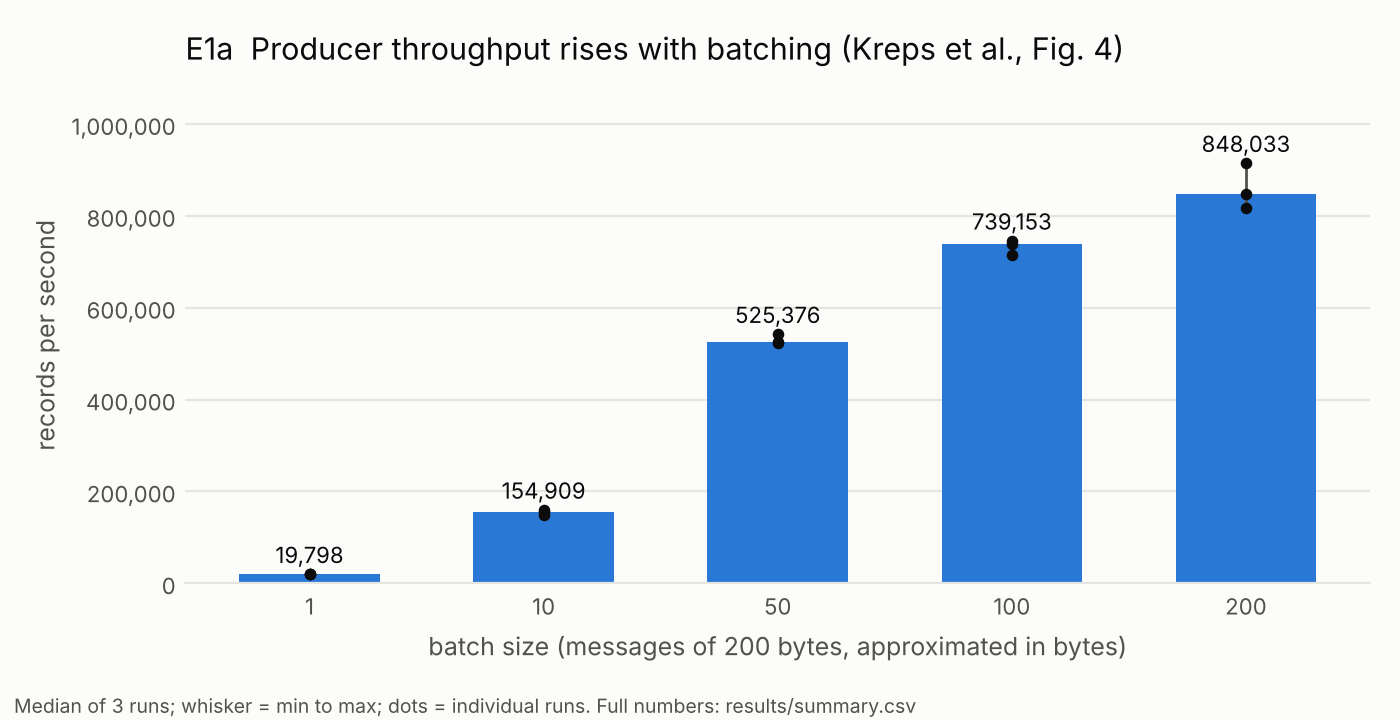
\includegraphics[width=0.8\textwidth]{e1a_producer_batching.png}
\caption{E1a: batching raises producer throughput.}
\label{fig:e1a}
\end{figure}

\subsection{E1b: continuous versus micro-batch (reproduction of Armbrust et al., Figure 7)}
A stateless pass-through job copies one topic to another. In continuous mode with 4 partitions, median
latency was 43 to 83 ms from 5,000 to 40,000 records per second (p99 0.3 to 0.9 s). At 80,000 records per
second its four tasks saturated: p50 rose to 1.8 s and p99 to 6.9 s. Micro-batch mode with a 100 ms
trigger kept up with the highest rate we could generate, at least 100,000 records per second, with
p50 between 0.27 and 0.62 s. See Figure~\ref{fig:e1b}.

\begin{figure}[H]
\centering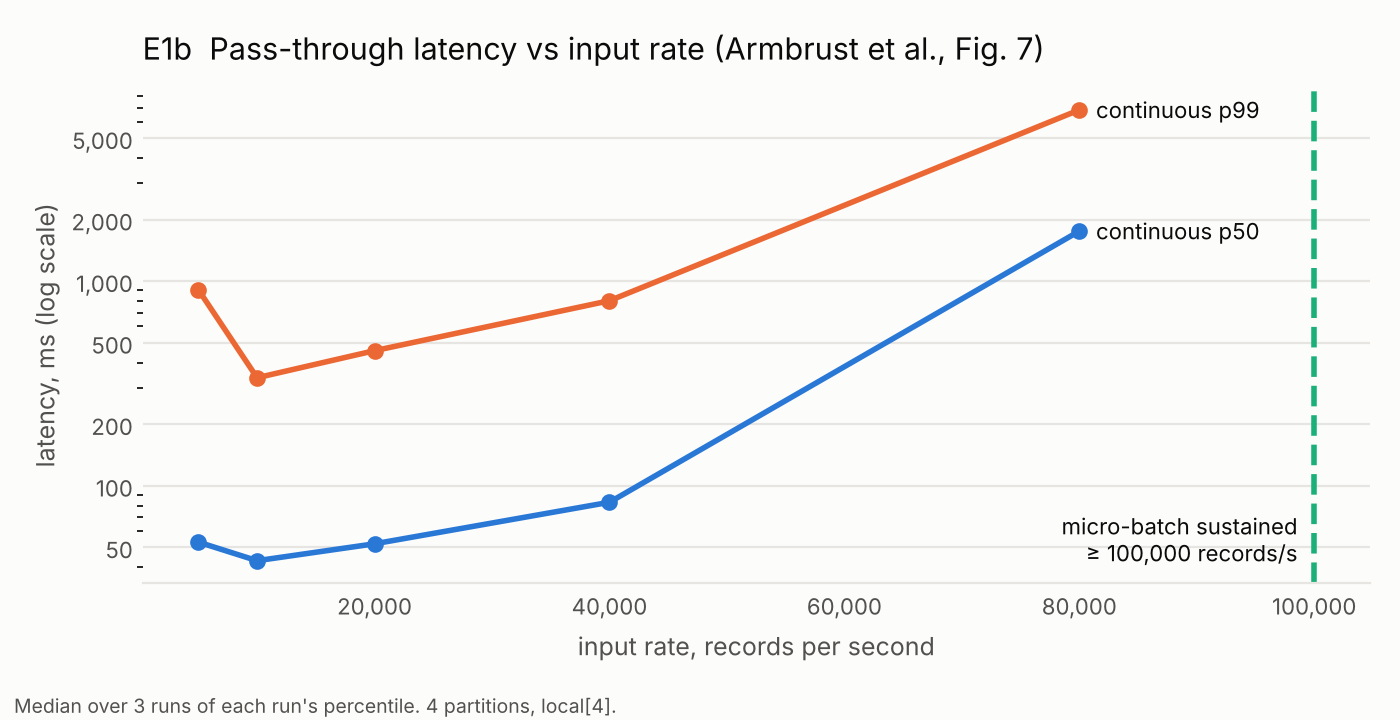
\includegraphics[width=0.85\textwidth]{e1b_continuous_vs_microbatch.png}
\caption{E1b: continuous mode has the lower latency until it saturates; micro-batch sustains a higher rate.}
\label{fig:e1b}
\end{figure}

\subsection{E1c: partitions and trigger interval (RQ1)}
Here we ran the real bars job in five-minute steps at 30,000, 60,000 and 90,000 records per second.
One partition sustained 75,000 records per second (one of three runs passed 90,000). Three and six
partitions, and every trigger from 500 ms to 5 s, sustained at least 90,000, which is the most our
generator could supply while sharing four cores with Spark. The 100 ms trigger reached its limit in one run of
three, at 75,000. Figure~\ref{fig:e1c-tp} shows this.

\begin{figure}[H]
\centering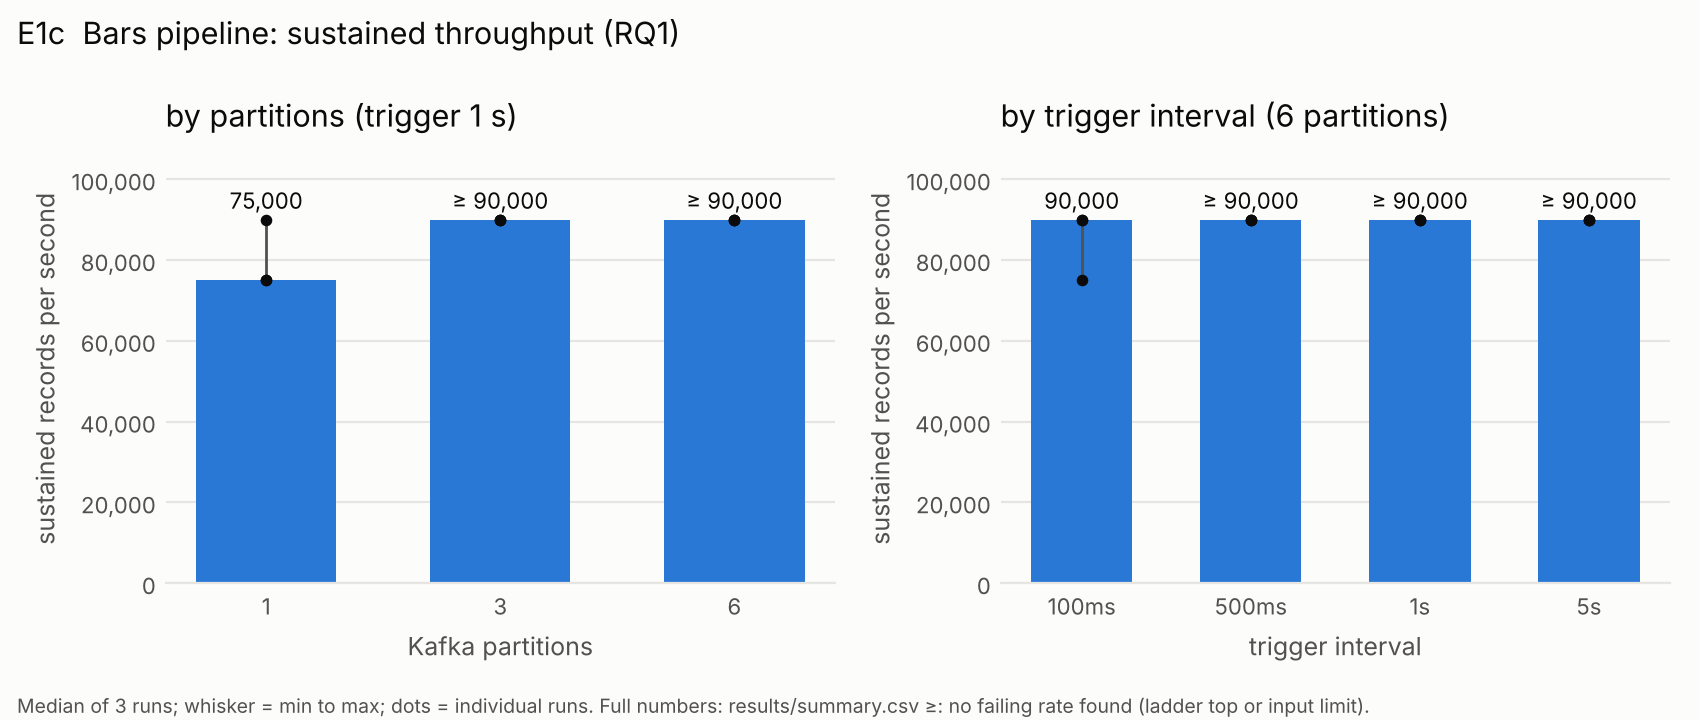
\includegraphics[width=0.85\textwidth]{e1c_sustained_throughput.png}
\caption{E1c: sustained throughput by partition count and trigger. Bars marked with a lower bound reached
our input limit before Spark's.}
\label{fig:e1c-tp}
\end{figure}

Bar latency runs from the window end plus the watermark to the moment the row is written.
Table~\ref{tab:e1c} gives the median p50.

\begin{table}[H]
\centering\small
\caption{E1c: bar latency p50 in seconds. The two sweeps ran on different CPUs (machine B, 2.30~GHz, and
machine A, 2.10~GHz), so we compare values only within one row.}
\label{tab:e1c}
\begin{tabular}{@{}lrr@{}}
\toprule
Setting & 30,000 records/s & 60,000 records/s \\
\midrule
1, 3, 6 partitions, trigger 1 s (machine B) & 2.5, 2.4, 2.5 & 2.4, 2.1, 3.5 \\
Trigger 100 ms, 500 ms, 1 s, 5 s, 6 partitions (machine A) & 2.2, \textbf{1.7}, 2.9, 7.2 & 6.4, 5.7, \textbf{4.9}, 8.7 \\
\bottomrule
\end{tabular}
\end{table}

The best trigger depends on the load. At 30,000 records per second a 500 ms trigger is fastest. At
60,000 a batch takes about two seconds whatever the trigger (batch duration p50 2.4 s at 100 ms, 2.1 s
at 500 ms, 2.0 s at 1 s), so a shorter trigger no longer starts batches sooner and only adds
per-batch overhead. There 1 s wins. A 5 s trigger always waits the longest. Below saturation the partition
count matters little, and at 60,000 six partitions on four cores cost more than three, because each
batch has more tasks and more state-store work. See Figures~\ref{fig:e1c-30} and~\ref{fig:e1c-60}.

\begin{figure}[H]
\centering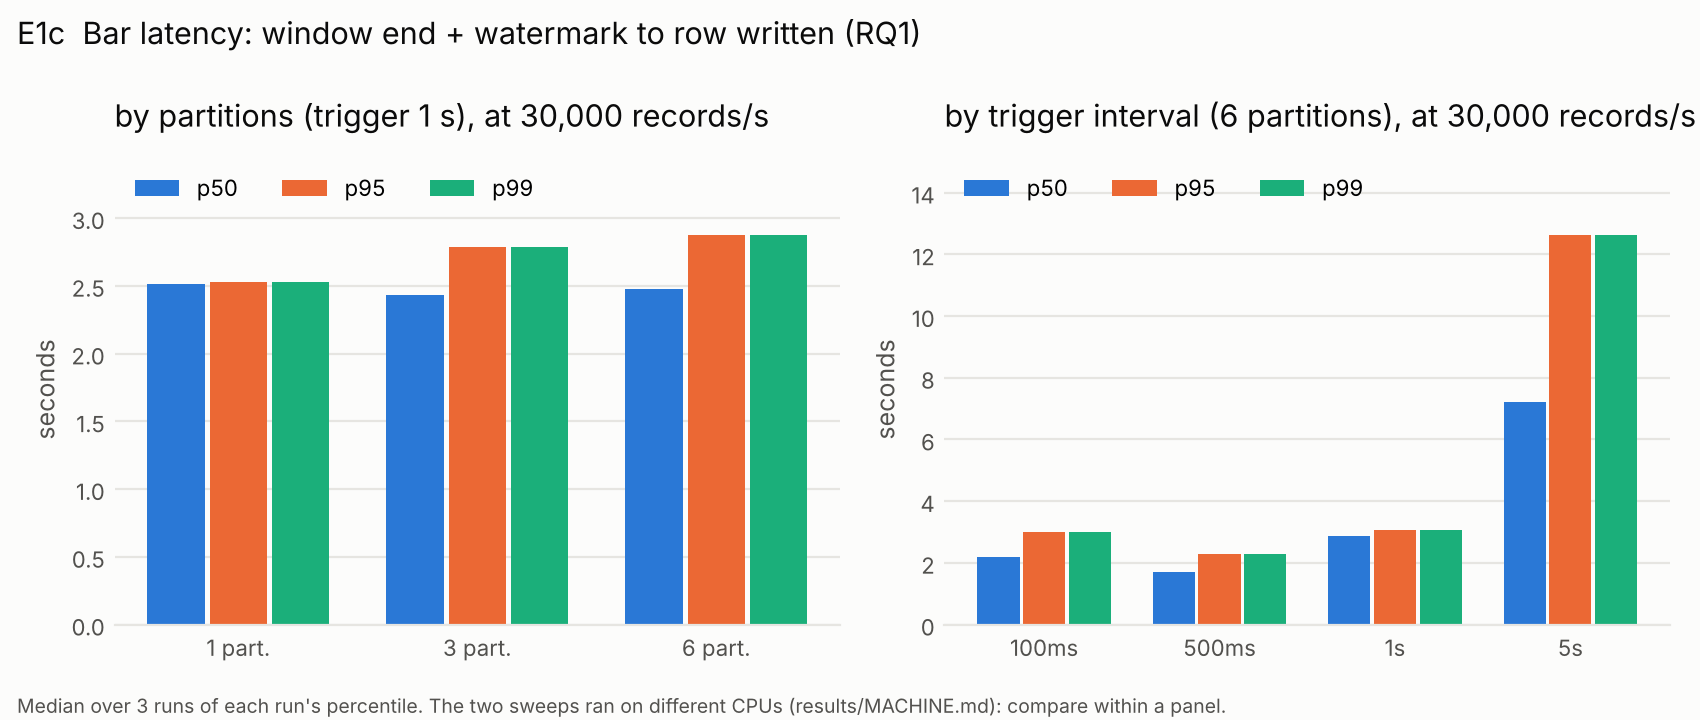
\includegraphics[width=0.85\textwidth]{e1c_bar_latency_30k.png}
\caption{E1c: bar latency at 30,000 records per second.}
\label{fig:e1c-30}
\end{figure}
\begin{figure}[H]
\centering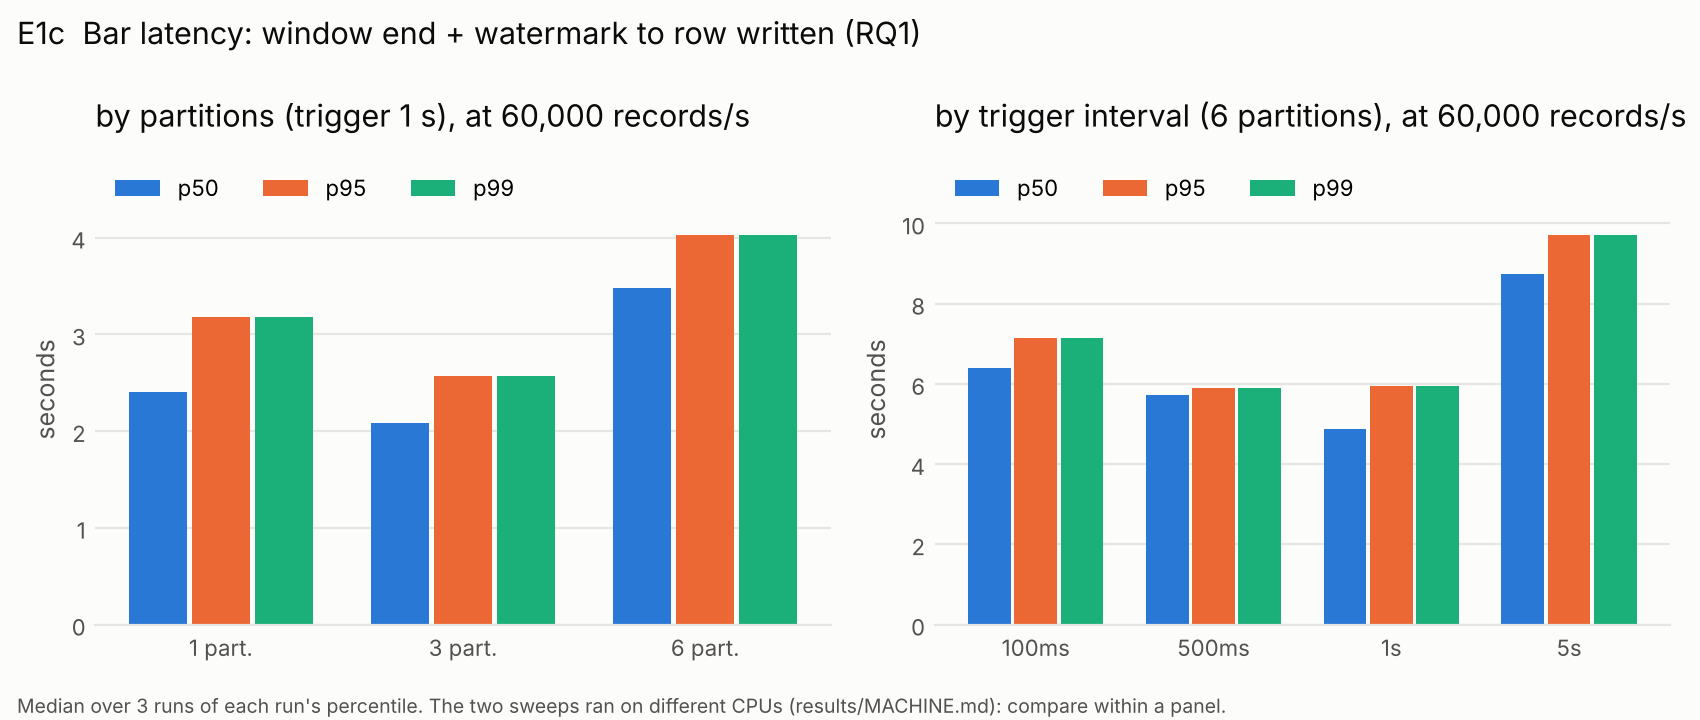
\includegraphics[width=0.85\textwidth]{e1c_bar_latency_60k.png}
\caption{E1c: bar latency at 60,000 records per second.}
\label{fig:e1c-60}
\end{figure}

\subsection{E2: broker crash (RQ2)}
We killed the broker that led partition 0 halfway through a 40-minute virtual run, with acks=1, with
acks=all, and with acks=all but no idempotence. No acknowledged trade was lost in any of the 12 kills.

With acks=all, writes stalled for 9.3 s [8.1 to 9.5] on every partition. The longest gap with no
acknowledgement anywhere was 9.1 s. The reason is that the dead broker stays in every partition's ISR
until the controller fences it, which takes the 9 s \code{broker.session.timeout.ms}. With acks=1 only the
partitions the dead broker led stalled, for 10.3 s [9.3 to 12.4], and the other partitions kept
acknowledging (longest gap anywhere 0.08 s). No duplicates appeared in these runs, even without
idempotence, although an earlier fault check did produce one (Section~\ref{sec:challenges}). A dry run
at a different rate did lose 2 acknowledged trades with acks=1, so loss is possible but rare.

One of the three runs without idempotence produced 33 wrong bars in a single minute even though Kafka
held every trade. The partitions resumed 3.8 s apart, the experiment's tenfold time compression turned
that into far more than the 10 s watermark, and Spark dropped those trades as late. This is a
real interaction between failover and watermarks, and we come back to it in Section~\ref{sec:limits}.
Figure~\ref{fig:e2} shows the stalls.

\begin{figure}[H]
\centering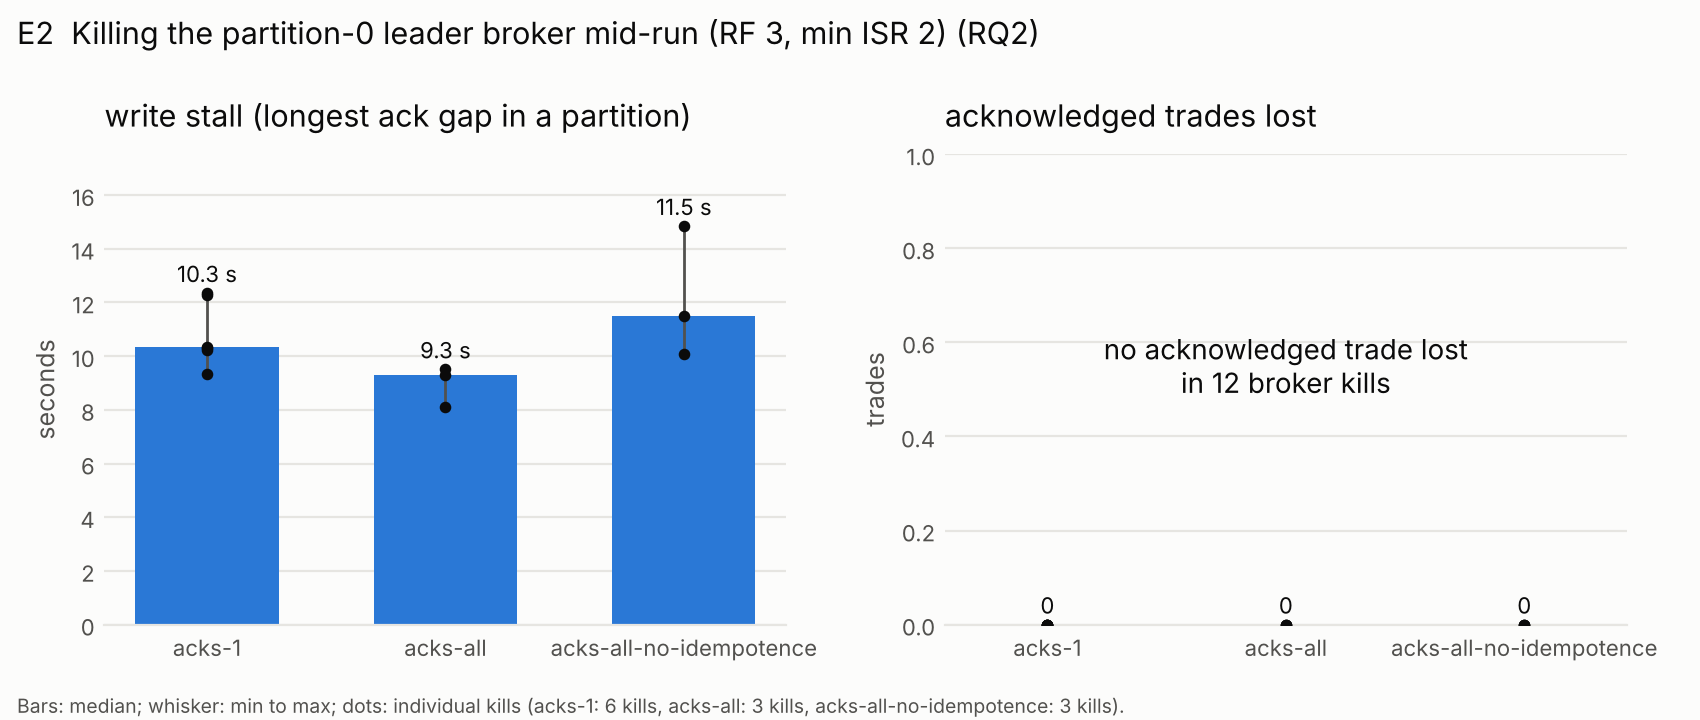
\includegraphics[width=0.9\textwidth]{e2_broker_crash.png}
\caption{E2: write stall and lost trades after a leader kill.}
\label{fig:e2}
\end{figure}

\subsection{E3: Spark crash (RQ2)}
We sent SIGKILL to the Spark container and restarted it at once on the same checkpoint. The first new bar
appeared 12.8 s [12.6 to 12.9] later in deterministic replay and 14.6 s [14.2 to 14.9] later on a live
stream, and the output was exact in all six runs. Almost all of that time is JVM and Spark start-up:
the first completed batch came 12.8 to 13.4 s after the restart. See Figure~\ref{fig:e3}.

\begin{figure}[H]
\centering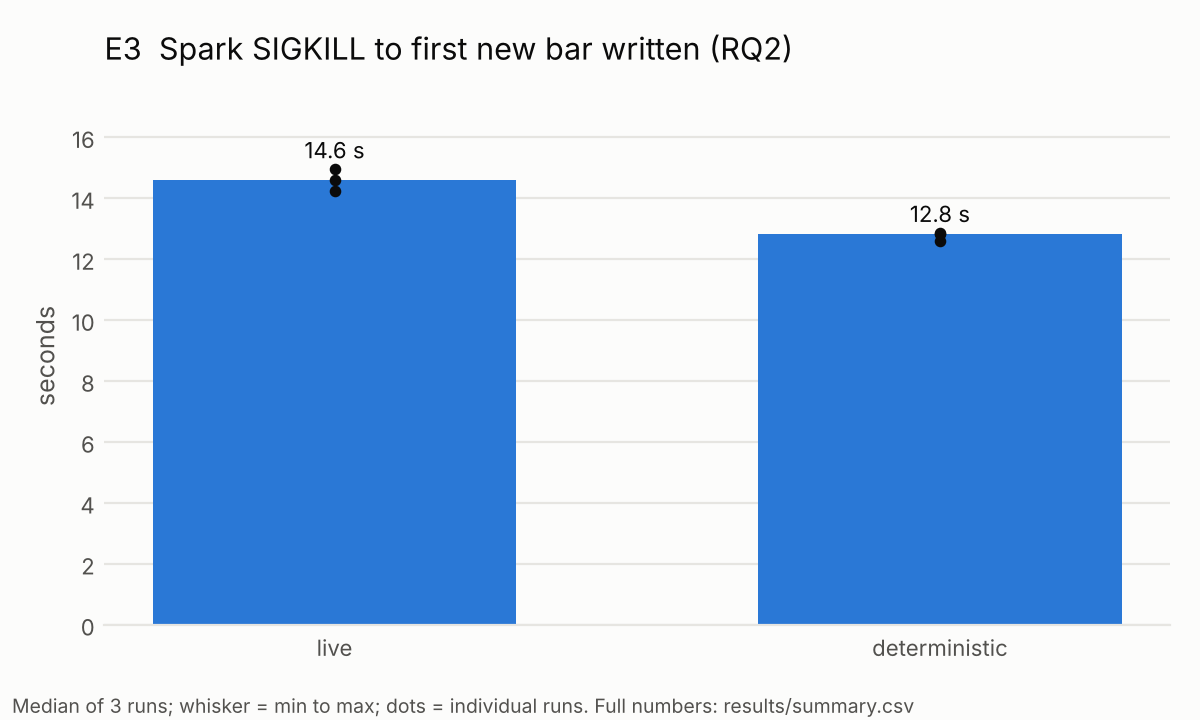
\includegraphics[width=0.7\textwidth]{e3_spark_recovery.png}
\caption{E3: time from the kill to the first new bar.}
\label{fig:e3}
\end{figure}

\subsection{E4: cost of exactly-once output (RQ3)}
We made Spark kill itself after the database commit and before Spark recorded the batch, so the restart
replays a batch that is already in the database. With plain inserts this left 300 duplicate bar rows in every
run, and with upserts none (three runs each). Without a crash, at 2,000 records per second, we could
not measure a cost for upserting. Batch duration p50 was 460 ms for inserts and 451 ms for upserts. Bar
latency p50 was 1.7 s [1.5 to 1.9] against 2.1 s [1.7 to 2.3], with overlapping ranges, and p99 was
2.45 s against 2.43 s. Both kept up. Figure~\ref{fig:e4} shows the results.

\begin{figure}[H]
\centering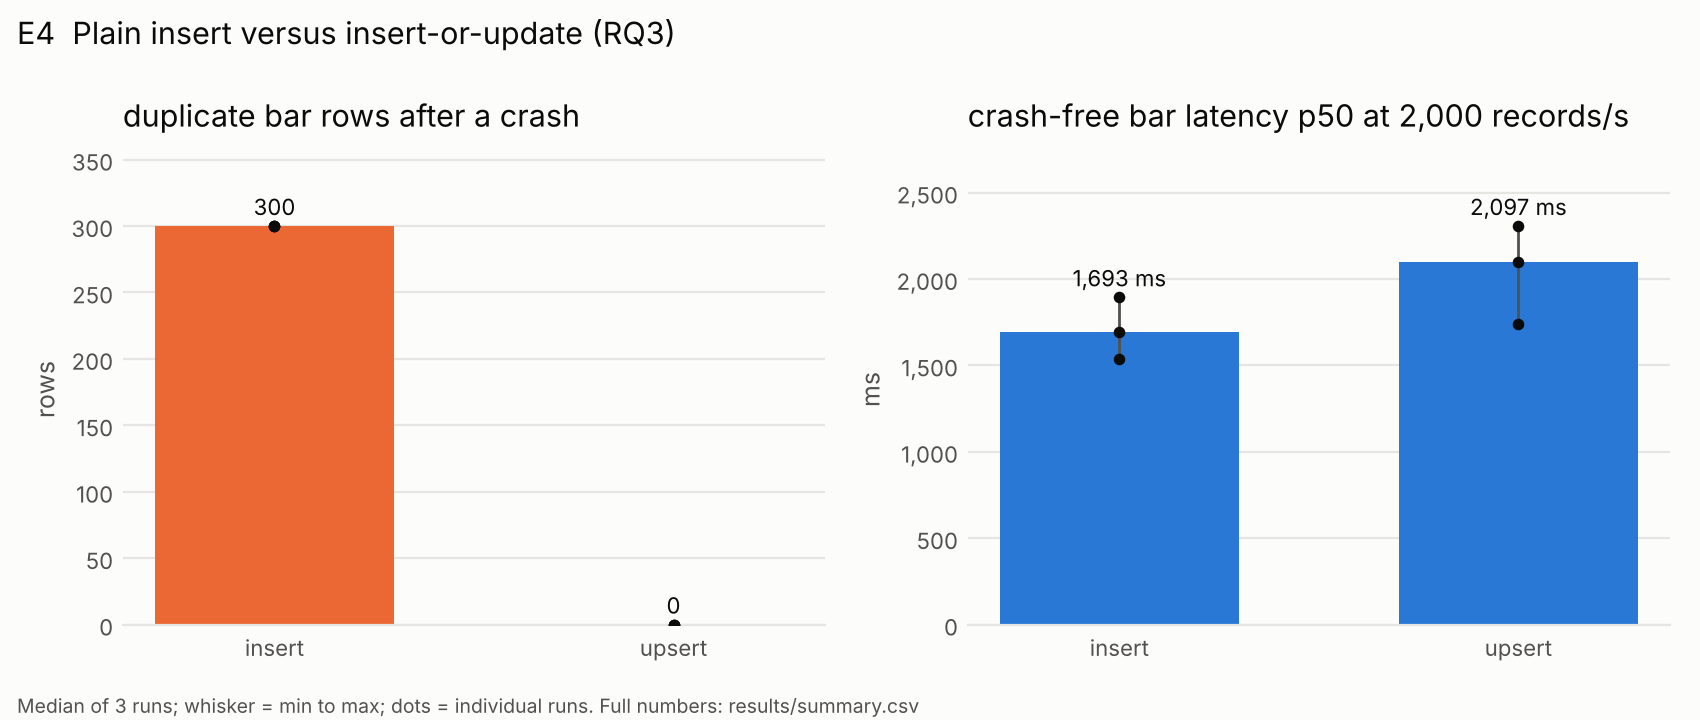
\includegraphics[width=0.9\textwidth]{e4_exactly_once.png}
\caption{E4: duplicate rows after a crash, and the cost of upserts without one.}
\label{fig:e4}
\end{figure}

\subsection{Live Coinbase run}
\label{sec:live}
We also ran the pipeline on live trades from Coinbase's public market-data feed for ten products (BTC, ETH,
SOL, XRP, DOGE, ADA, AVAX, LINK, LTC and BCH), on a Windows laptop with Docker Desktop, for more than 20
minutes. The producer connected to the feed, sent every trade to Kafka with acks=all, and saved a capture. The
dashboard filled with one-minute bars for all ten symbols, with Spark's lag at zero. No alert fired, which is
expected: live prices rarely move three standard deviations from their previous 30 one-minute returns, while the
synthetic data injects such shocks on purpose. After stopping the producer we ran the verifier against the
topic's own contents, because no generator file exists for live data. All 230 bars matched exactly (none
missing, extra, duplicated or different), and there were no alerts to match.

%------------------------------------------------------------------------------------------------
\section{Discussion: reproduction and extension}
\paragraph{Reproduction (a).} Batching raises producer throughput by more than an order of magnitude,
as Kreps et al.\ found, so the shape holds. Our unbatched rate is lower than theirs because every
one-record request is a round trip on a single shared four-core machine, and our batched rates are
higher because the producer and the CPU are newer. The paper used two dedicated 8-core machines, and we
approximate a batch of $n$ messages as $n \times 200$ bytes, since the Java producer sizes batches in bytes.

\paragraph{Reproduction (b).} Continuous processing gives much lower latency (tens of milliseconds
against hundreds) up to a saturation point, past which its latency climbs steeply, while micro-batch
sustains a higher input rate. The shape matches Armbrust et al. Their continuous latency was about
1 ms, and ours is tens of milliseconds because ours includes the producer's batching (\code{linger.ms}
of 5), a Kafka write with acks=all on three replicas, and the sink's own producer. The limit of one
core per partition on four cores is the constraint the paper describes, and we hit it.

\paragraph{Extension.} For RQ2, with replication factor 3 and a minimum ISR of 2, no acknowledged trade
was lost in 12 leader kills. The price of acks=all is a stall of about 9 s on every partition until the
dead broker is fenced. Acks=1 confines the stall to the dead broker's partitions but can lose
acknowledged writes, which we saw once, in a dry run. Spark recovers from its own crash in 13 to 15 s
with exact output. For RQ3, plain inserts are wrong after a crash (300 duplicate rows every time), and upserts
are exact at no cost we could measure at 2,000 records per second.

%------------------------------------------------------------------------------------------------
\section{Challenges}
\label{sec:challenges}
\begin{enumerate}
  \item \textbf{Determinism against late data.} An unpaced replay squeezes 40 virtual minutes into a few
        seconds, so a few milliseconds of skew between partitions looked like more than the 10 s watermark
        and trades would have been dropped as late. We now preload the topic before Spark starts.
  \item \textbf{Duplicates from producer retries.} With acks=all but idempotence off, killing a leader made
        the producer write one trade twice, and the verifier caught the wrong bar. Idempotence is now the
        default, and E2 measures the difference.
  \item \textbf{Measuring a write stall.} Looking at all partitions together hid the acks=1 behavior.
        We now compute the stall per partition from timestamped acknowledgements.
  \item \textbf{JVM warm-up} made the first latencies about twenty times worse, so we discard a warm-up
        period.
  \item \textbf{Continuous mode needs a core per partition.} With 6 partitions on 4 cores, two partitions were
        never processed, with no error. Continuous runs use 4 partitions.
  \item \textbf{Crashing between two commits.} A SIGKILL sent to PID 1 inside a container is ignored. The fault
        hook needed an init process and a kill of the driver JVM from inside \code{foreachBatch}.
  \item \textbf{Floating-point equality.} Fractional crypto sizes summed in a different order differ in
        the last bits, so the verifier allows a relative $10^{-9}$ for volume only.
  \item \textbf{Versions and tooling.} We checked that Kafka 4.4, Spark 4.2, PostgreSQL 18 and Grafana 13
        exist before pinning them, and had to build images behind a TLS-inspecting proxy and around Docker
        Hub rate limits.
  \item \textbf{Live data access.} The cloud development environment could not reach the Coinbase feed, so we
        first tested the adapter against a fake server that follows the protocol, and from captured sessions. We
        later ran it on a laptop (Section~\ref{sec:live}). Getting the stack to start on Windows took four fixes
        (a Linux-only default path, a missing image build, and two host ports that Windows had reserved or
        another project was using).
\end{enumerate}

%------------------------------------------------------------------------------------------------
\section{Reproducibility}
\label{sec:repro}
The repository holds everything needed to repeat the work. \code{docker compose up} starts the pipeline
and the demo. Image tags and Python packages are pinned and locked. A golden dataset with a SHA-256
manifest lets \code{make golden} replay a known stream through Kafka and Spark and check every bar and
alert against the oracle. \code{make bench-all} runs every experiment (about 12 hours), and
\code{uv run python -m bench.summarize} rebuilds every table and figure from the raw runs. Each run stores
its parameters, versions, git commit and machine. Continuous integration runs the linter, the unit tests and
the PostgreSQL integration tests on every push. The README explains how to run each step.

%------------------------------------------------------------------------------------------------
\section{Limitations: what one machine can and cannot show}
\label{sec:limits}
All three brokers, Spark (\code{local[4]}), PostgreSQL, Grafana, the generator and the measuring harness
ran on one virtual machine with 4 CPUs and 16 GB. Every container shares those four cores, one disk and
the loopback network. Our results are therefore sound for what they compare on this machine and weak as
absolute numbers.

\subsection{Throughput}
\begin{itemize}
  \item \textbf{Components compete for the same CPUs.} A measured rate is the pipeline's capacity while the
        generator, three brokers and PostgreSQL also run. On a cluster Kafka, Spark and the producers would
        have their own cores and every rate here would probably be higher. We report sustained rates as
        properties of this machine, not as limits of Kafka or Spark.
  \item \textbf{Our input is itself a ceiling.} The Python generator tops out near 100,000 records per second
        while Spark runs beside it. ``At least 90,000'' and ``micro-batch kept up at 100,000'' mean that the
        pipeline did not saturate before our input did. The true maximum is unknown.
  \item \textbf{Partition scaling is capped by cores.} More partitions than cores did not help (E1b, E1c). That
        shows the four-core limit and says nothing about how Kafka scales. The benefits of partitions in
        production, such as consumers on many machines and many disks, cannot appear here.
  \item \textbf{No network cost.} Replication between brokers crosses the loopback interface, so the latency of
        acks=all, which waits for replicas over a real network, is understated. E1a also differs from the
        paper because producer and broker share cores, where the paper used two 8-core machines.
  \item \textbf{One disk and the page cache.} Kafka depends on sequential disk writes and the page cache.
        Three brokers on one volume cannot show per-broker disk limits, and we did not enable \code{fsync}.
  \item \textbf{Changing hardware.} The virtual machine's CPU changed from 2.30 to 2.10 GHz between two
        experiments. We added a baseline setting (\code{p6-1s-b}) and compare triggers only within one machine
        state. Three runs per setting give a range, not a confidence interval.
  \item \textbf{Synthetic data.} Every measurement uses the seeded generator. Live Coinbase data appears only
        in the demonstration and in the short run of Section~\ref{sec:live}.
\end{itemize}

\subsection{Fault tolerance}
\begin{itemize}
  \item \textbf{A killed container is not a failed node.} \code{docker kill} stops one broker process at once.
        It does not model a network partition, a slow or full disk, a failed rack, a lost machine, or two
        brokers failing together. With three brokers on one host, the host is a single point of failure that
        none of our experiments can survive.
  \item \textbf{Detection time is configuration, not network behavior.} The 9 s stall in E2 equals the
        controller's \code{broker.session.timeout.ms} of 9,000 ms. On a real network, detection also depends on
        latency, partitions and clocks, and the stall could be shorter if tuned, or longer. We measured how this
        configuration reacts to a clean kill, not how fast Kafka recovers in general.
  \item \textbf{We injected the favorable failure.} A crashed leader's followers hold identical data, so a
        minimum ISR of 2 with unclean election off loses nothing. A leader that stays up but is cut off from
        its followers would test those settings harder, and we cannot produce that here.
  \item \textbf{Spark recovery excludes a cluster.} \code{local[4]} has no executors to lose, no rescheduling and
        no network shuffle. E3 measures checkpoint recovery of the driver (JVM start, state restore and
        replay), which is real, but not recovery on a standalone, YARN or Kubernetes cluster.
  \item \textbf{Time compression magnifies skew.} The crash experiments run virtual time ten times faster than
        the wall clock. A failover skew of a few seconds between partitions became tens of seconds of event
        time and made the 10 s watermark drop trades in one run (Section~\ref{sec:results}). With real-time data
        the same skew is ten times smaller relative to the watermark, so the failure would be rarer. The
        lesson that the watermark must exceed the partition skew still holds.
  \item \textbf{One local database.} A single PostgreSQL on the same machine has no network round trip and no
        competing writers, so the upsert cost we measured at 2,000 records per second is a lower bound for a
        remote or shared database.
\end{itemize}

\subsection{What still holds}
The correctness results do not depend on the machine. The bars and alerts match the oracle in every run,
no acknowledged trade was lost, and the duplicate rows in E4 follow from the protocol: a crash between
the database commit and Spark's commit replays the batch. The relative comparisons made on one machine
state (batching against none, continuous against micro-batch, trigger intervals, insert against upsert)
are valid for that machine, and their shapes agree with the published papers. We described Kafka's
security features (TLS, SASL, ACLs) but did not measure them. The harness could be pointed at a
multi-node cluster to extend the study.

%------------------------------------------------------------------------------------------------
\section{Conclusion}
\paragraph{RQ1.} The processing mode sets the latency floor. Continuous processing answers in tens of
milliseconds but saturates between 40,000 and 80,000 records per second on four cores, while micro-batch
trades hundreds of milliseconds for at least 100,000 records per second. For the bars pipeline the
trigger should match the load: 500 ms at moderate load, 1 s at high load, and 5 s was never best. More
partitions than cores did not help.

\paragraph{RQ2.} With replication factor 3 and a minimum ISR of 2, no acknowledged trade was lost in 12
leader kills. Acks=all stalls all writes for about 9 s until the dead broker is fenced, and acks=1 stalls
only its partitions but can lose acknowledged writes. A failover can also make Spark drop trades as late
when the watermark is shorter than the skew between partitions. Spark recovers from its own crash in
about 13 to 15 s with exact output.

\paragraph{RQ3.} Exactly-once output needs an idempotent sink. Plain inserts duplicated 300 rows after
every crash between the database commit and Spark's commit, upserts duplicated none, and at 2,000 records
per second the upsert cost nothing measurable.

\bibliographystyle{unsrt}
\bibliography{references}

%------------------------------------------------------------------------------------------------
\appendix
\section{Configuration of each experiment}
\label{app:config}
These tables come from \path{docker-compose.yml}, the topic script, the generator's defaults and the
experiment definitions in \path{bench/experiments/}. Each run also stores its own parameters in
\path{config.json} next to its raw output.

\subsection{Settings shared by all experiments}
\begin{table}[H]
\centering\small
\caption{Stack settings.}
\begin{tabularx}{\textwidth}{@{}>{\raggedright\arraybackslash}p{3.2cm}Y@{}}
\toprule
Component & Setting \\
\midrule
Kafka brokers & Image \code{apache/kafka:4.4.0}; 3 nodes, each broker and controller (KRaft combined mode); heap 1 GB per broker; \code{default.replication.factor=3}; \code{min.insync.replicas=2}; \code{unclean.leader.election.enable=false}; \code{auto.create.topics.enable=false}; PLAINTEXT listeners; no \code{log.flush.*} override; failure detection at the defaults (session timeout 9,000 ms, heartbeat 2,000 ms). \\
Topics & \code{trades}: 6 partitions by default (set per experiment), RF 3, min ISR 2, retention 1 day. \code{passthrough\_out}: same partitions as \code{trades}, RF 3, min ISR 2, \code{LogAppendTime}, retention 1 day. \code{perf\_test}: 1 partition, RF 1, min ISR 1, retention 1 hour. \\
Spark & Image \code{spark:4.2.1-scala2.13-java17-python3-ubuntu} with the Kafka connector \code{spark-sql-kafka-0-10\_2.13:4.2.1}; \code{--master local[4]}; driver memory 2 GB; container limit 4 CPUs and 3 GB; \code{spark.sql.shuffle.partitions=4}; session time zone UTC; \code{failOnDataLoss=true}; checkpoints on a named volume. \\
Bars job & Trigger 1 s; watermark 10 s; sink mode upsert; \code{startingOffsets=earliest}. \\
Pass-through job & Micro-batch trigger 100 ms, or continuous with a 1 s checkpoint interval; \code{startingOffsets=latest}. \\
PostgreSQL & Image \code{postgres:18.6}. \\
Producer (\code{confluent-kafka}) & \code{linger.ms=5}; \code{batch.size=1000000}; \code{retries=2147483647}; \code{queue.buffering.max.messages=500000}; \code{acks=all} with \code{enable.idempotence=true}, except where an experiment says otherwise (idempotence cannot be combined with acks=1). \\
\bottomrule
\end{tabularx}
\end{table}

\subsection{Settings per experiment}
\begin{table}[H]
\centering\footnotesize
\caption{Per-experiment settings. ``Records/s'' is the input rate.}
\begin{tabularx}{\textwidth}{@{}>{\raggedright\arraybackslash}p{1.1cm}YYY@{}}
\toprule
 & Kafka & Spark & Producer and input \\
\midrule
E1a & \code{perf\_test}: 1 partition, RF 1, min ISR 1; topic recreated for each setting & None & \code{kafka-producer-perf-test} inside \code{kafka-1}, 10 million records of 200 bytes, unlimited rate, \code{acks=0}; \code{batch.size} 0, 2,000, 10,000, 20,000, 40,000 bytes; \code{linger.ms} 0 (batch 1) or 10 \\
E1b & \code{trades} and \code{passthrough\_out}: 4 partitions, RF 3, min ISR 2 & Pass-through job; continuous (1 s checkpoint) or micro-batch (100 ms trigger); \code{startingOffsets=latest} & Realtime, \code{acks=all}, idempotent; continuous at 5,000, 10,000, 20,000, 40,000 and 80,000 records/s for 120 s (20 s warm-up); micro-batch at 40,000, 80,000 and 100,000 for 300 s (30 s warm-up) \\
E1c & \code{trades}: 1, 3 or 6 partitions, RF 3, min ISR 2; recreated before each step & Bars job, upsert sink; trigger 100 ms, 500 ms, 1 s or 5 s; \code{startingOffsets=latest} & Realtime, \code{acks=all}, idempotent, no closing trade; 30,000, 60,000 and 90,000 records/s, 300 s per step, 70 s warm-up; settings p1, p3, p6 with a 1 s trigger, and p6 with 100 ms, 500 ms, 5 s, plus a repeat of p6 at 1 s \\
E2 & \code{trades}: 6 partitions, RF 3, min ISR 2; the leader of partition 0 killed at 50\% of the run & Bars job, trigger 1 s, \code{startingOffsets=earliest} & Virtual mode, seed 42, 40 virtual minutes at 10 times speed, 1.0 trades per symbol per virtual second; acks=all with idempotence (3 kills), acks=1 (6 kills), acks=all without idempotence (3 kills) \\
E3 & \code{trades}: 6 partitions, RF 3, min ISR 2 & Bars job; SIGKILL at 50\% of the stream (live) or after batch 5 (deterministic, \code{maxOffsetsPerTrigger=5000}); restart at once on the same checkpoint & Live: virtual mode, seed 42, 40 minutes at 10 times speed. Deterministic: golden dataset (60,163 trades) preloaded and replayed at maximum speed. \code{acks=all}, idempotent \\
E4 & \code{trades}: 6 partitions, RF 3, min ISR 2 & Bars job; sink insert (\code{bars\_plain}) or upsert (\code{bars}); crash runs use \code{FAULT\_AFTER\_BATCH=5} and \code{maxOffsetsPerTrigger=5000} & Crash runs: golden replay. Cost runs: realtime at 2,000 records/s for 300 s, 70 s warm-up, no crash \\
\bottomrule
\end{tabularx}
\end{table}

\section{Machine and versions}
\label{app:machine}
Runs started on 11 November 2026 and finished on 12 November 2026 (72 runs, none failed). The development
virtual machine was moved between physical hosts when it restarted, so two CPUs appear. Both are 4-vCPU Intel
Xeon virtual machines with 15.7 GB of memory, Docker 29.9.2 and Linux 6.18.44: machine A at 2.10 GHz and
machine B at 2.30 GHz. Table~\ref{tab:machines} says which experiments ran where, and results are compared
only within one machine.

\begin{table}[H]
\centering\small
\caption{Where each experiment ran.}
\label{tab:machines}
\begin{tabular}{@{}ll@{}}
\toprule
Machine & Settings \\
\midrule
A (2.10 GHz) & E1c p6-100ms, p6-500ms, p6-5s and p6-1s-b; E2 (all); E3 (all); E4 crash runs \\
B (2.30 GHz) & E1a (all); E1b (all); E1c p1-1s, p3-1s and p6-1s; E4 cost runs \\
\bottomrule
\end{tabular}
\end{table}

\noindent Software: Apache Kafka 4.4.0, Apache Spark 4.2.1 (PySpark, Python 3.10 in the image), PostgreSQL
18.6, Grafana 13.3.0; on the host Python 3.13, confluent-kafka 2.16.1, psycopg 3.3.8, numpy 2.5.3 and
pandas 3.0.5, all pinned in the repository's lock file.

%   3. Add the packages below to the template's preamble if it does not load them already:
%        booktabs, tabularx, array, graphicx, float, caption, enumitem, tikz (with libraries
%        positioning, arrows.meta, shapes.geometric, fit, backgrounds), xurl, hyperref
%        and this macro:   \newcommand{\code}[1]{\texttt{#1}}
%        and this column type:   \newcolumntype{Y}{>{\raggedright\arraybackslash}X}
%        and:   \graphicspath{{figures/}}
%   4. If the template sets up its own bibliography, delete the two lines near the end of this file
%      (\bibliographystyle and \bibliography) and keep the template's.
%
% report/main.tex is a ready-made wrapper that does exactly this, so it compiles on its own.

\begin{abstract}
Trading desks want per-minute summaries and alerts within seconds of each trade. We built that
pipeline from Apache Kafka 4.4 (three brokers, KRaft) and Spark 4.2 Structured Streaming (PySpark).
It writes one-minute open, high, low, close and volume-weighted average price (VWAP) bars and
three-sigma alerts to PostgreSQL, shows them in Grafana, and starts with one \code{docker compose up}.
A seeded generator makes the correct output known exactly, so we check every run bar by bar. We
reproduce two published results, producer batching (Kreps et al., Figure 4) and continuous versus
micro-batch latency (Armbrust et al., Figure 7), and add what neither paper measured: whether the output
stays correct when a broker or the Spark job crashes, and what exactly-once output costs. No
acknowledged trade was lost in 12 broker crashes. Spark recovered from its own crash in about 14
seconds with exact output. Plain inserts left 300 duplicate rows after every crash, while upserts left
none and cost nothing we could measure at 2,000 trades per second. All measurements come from one
4-CPU machine, and Section~\ref{sec:limits} says what that does to the conclusions.
\end{abstract}

%------------------------------------------------------------------------------------------------
\section{Background and significance}
Market data arrives as a continuous stream of trades. A common design pairs a durable, partitioned
log that stores the events with a stream processor that reads the log and computes results over time
windows.

\paragraph{Apache Kafka.} Kafka~\cite{kreps2011,wang2015} is the log. A topic is split into
partitions, and each partition is an append-only file on a broker, written and read sequentially in
batches. Kreps et al.\ showed that this gives much higher throughput than traditional message
queues~\cite{kreps2011}. Kafka orders events only within a partition, so keying trades by symbol keeps
each symbol's trades in order. Each partition is copied to several brokers: a leader serves reads and
writes, and the followers that are caught up form the in-sync replica set (ISR). Whether an acknowledged
write survives a broker crash depends on three settings: the replication factor, the number of copies
the producer waits for (\code{acks}), and the minimum number of in-sync replicas~\cite{wang2015}. Kafka 4
keeps cluster metadata in its own Raft-based protocol (KRaft), so it no longer needs ZooKeeper.

\paragraph{Spark Structured Streaming.} Structured Streaming~\cite{armbrust2018} is the processor. It
treats a stream as an unbounded table and runs a normal SQL-style query over it incrementally, usually
in micro-batches, an approach that descends from discretized streams~\cite{zaharia2013}. It aggregates
over event-time windows and keeps intermediate state between batches. A watermark says how long Spark
waits for late events before it finalizes a window, an idea from the Dataflow model~\cite{akidau2015}.
Spark records each batch's Kafka offsets and its state in a checkpoint. Kafka can re-deliver from any
offset, so after a crash Spark re-runs exactly the unfinished batches, and an idempotent sink then makes
the result the same as if each event had been processed once. An experimental continuous mode lowers
latency, but it supports only per-record operations and delivers at least once.

\paragraph{Why test them together.} The papers promise high throughput from batched sequential I/O,
durability from replication, and exactly-once results from replay plus checkpoints. Each promise
depends on configuration and on how the two systems are connected. We test them on a financial
workload with a known correct answer, and we focus on the seam between the systems more than on either
one alone.

%------------------------------------------------------------------------------------------------
\section{Goals and objectives}
We set out to answer three research questions.
\begin{enumerate}[label=\textbf{RQ\arabic*.},leftmargin=*]
  \item How do the number of partitions, the trigger interval and the processing mode trade latency
        against throughput?
  \item Which Kafka settings prevent lost or duplicated data when a broker crashes, and how long does
        Spark take to recover from its own crash?
  \item What does exactly-once output cost compared with at-least-once output?
\end{enumerate}
The objectives are: (1) explain how Kafka, Spark and their integration work; (2) build a case-study
pipeline that starts with one command; (3) reproduce Kreps et al.\ Figure~4 and Armbrust et al.\
Figure~7, comparing the shape of each curve and not the absolute numbers; (4) extend both papers with
experiments they did not run, namely correctness under crashes and the cost of exactly-once output;
and (5) publish a repository that others can run, with pinned versions and scripted experiments.

%------------------------------------------------------------------------------------------------
\section{Architecture analysis}
\label{sec:arch}
Figure~\ref{fig:pipeline} shows the pipeline we built. A generator publishes trades, keyed by symbol,
to a topic with six partitions. Spark reads one task per partition, builds one-minute bars with a
10-second watermark, and writes each batch to PostgreSQL in one transaction. Grafana reads PostgreSQL.

\begin{figure}[H]
\centering
\resizebox{\textwidth}{!}{%
\begin{tikzpicture}[
  node distance=9mm and 8mm,
  box/.style={draw,rounded corners=2pt,align=center,inner sep=4pt,font=\small,minimum height=10mm},
  store/.style={draw,cylinder,shape border rotate=90,aspect=0.25,align=center,font=\small,minimum height=11mm,inner sep=3pt},
  arr/.style={-{Stealth[length=2mm]},thick},
  lab/.style={font=\scriptsize,align=center}]
  \node[box] (gen) {Generator\\(seeded, or\\Coinbase live)};
  \node[box,right=26mm of gen] (kafka) {Kafka, 3 brokers\\topic \code{trades}\\6 partitions, RF 3,\\min ISR 2};
  \node[box,right=26mm of kafka] (spark) {Spark\\\code{local[4]}, 1 s trigger\\watermark 10 s,\\1-minute windows};
  \node[store,right=30mm of spark] (pg) {PostgreSQL\\bars, alerts};
  \node[box,right=12mm of pg] (graf) {Grafana};
  \node[store,below=8mm of spark] (ck) {Checkpoint\\volume};
  \draw[arr] (gen) -- node[lab,above]{key = symbol} node[lab,below]{acks=all} (kafka);
  \draw[arr] (kafka) -- node[lab,above]{one task per} node[lab,below]{partition} (spark);
  \draw[arr] (spark) -- node[lab,above]{one transaction} node[lab,below]{per batch} (pg);
  \draw[arr] (pg) -- (graf);
  \draw[arr,dashed] (spark) -- node[lab,right]{offsets, state} (ck);
\end{tikzpicture}}
\caption{The pipeline. A separate pass-through job (not shown) copies \code{trades} to a second
topic for the latency experiments.}
\label{fig:pipeline}
\end{figure}

\subsection{Kafka}
Table~\ref{tab:kafka} lists the Kafka mechanisms we rely on and where each one shows up in the project.

\begin{table}[H]
\centering\small
\caption{Kafka mechanisms and their role in this project.}
\label{tab:kafka}
\begin{tabularx}{\textwidth}{@{}>{\raggedright\arraybackslash}p{3.1cm}YY@{}}
\toprule
Mechanism & How it works & In this project \\
\midrule
Partitions and ordering & A partition is an append-only log on a broker, written and read sequentially. Order holds only within a partition; the producer picks the partition by hashing the key. & \code{trades} has 6 partitions on 3 brokers. Key = symbol, so every symbol lands in one partition and stays in order (checked from the acknowledgement log). \\
Throughput design~\cite{kreps2011} & Batching many records per request, sequential disk I/O, the page cache, zero-copy transfer. & E1a reproduces the batching effect. \\
Retention & Records stay for a time or size limit whether or not they were read, so a consumer can re-read from any offset. & \code{trades} keeps one day. Replay after a crash depends on it. \\
Replication and ISR~\cite{wang2015} & A partition has a leader and followers. A write is committed when every in-sync replica has it. & RF 3, \code{min.insync.replicas=2}, unclean leader election off, so only an in-sync replica can become leader. \\
Producer \code{acks} & 0: no wait. 1: the leader only. all: every in-sync replica. & E2 kills a leader with acks=1 and acks=all. \\
Idempotent producer & The broker drops a retried batch it has already seen, using the producer id and a sequence number. & On by default with acks=all. Without it, a leader kill once duplicated a trade (Section~\ref{sec:challenges}). \\
KRaft & Metadata lives in a Raft-replicated log on controller nodes. & Three nodes, each broker and controller. \\
Consumer groups & Consumers with one \code{group.id} split a topic's partitions, and Kafka stores the group's committed offsets. & Used by our verifier and latency collectors. Spark does not use them (Section~\ref{sec:integration}). \\
Delivery guarantees & At most once, at least once, or exactly once (idempotent producer plus transactions inside Kafka). & End-to-end exactly-once here comes from Spark's replay plus an idempotent sink. \\
Security & TLS encrypts traffic, SASL authenticates clients, ACLs authorize operations. & Described, not measured. The stack runs PLAINTEXT on one machine, with Grafana and PostgreSQL bound to localhost. \\
\bottomrule
\end{tabularx}
\end{table}

\subsection{Spark Structured Streaming}
Table~\ref{tab:spark} does the same for Spark.

\begin{table}[H]
\centering\small
\caption{Spark mechanisms and their role in this project.}
\label{tab:spark}
\begin{tabularx}{\textwidth}{@{}>{\raggedright\arraybackslash}p{3.1cm}YY@{}}
\toprule
Mechanism & How it works & In this project \\
\midrule
Unbounded table~\cite{armbrust2018} & A streaming query is an ordinary DataFrame query that Spark runs incrementally. The optimizer turns it into an incremental plan with stateful operators. & The bars job is a \code{groupBy(window, symbol)} aggregation. \\
Micro-batch and triggers~\cite{zaharia2013} & A trigger starts a batch at fixed intervals; each batch reads the offsets that arrived since the last one. & Trigger 1 s by default. E1c varies it from 100 ms to 5 s. \\
Continuous processing & Long-running tasks handle one record at a time and checkpoint in epochs. Lower latency, but only map-like operations, at-least-once, and one core per input partition. & Cannot run the bars job. E1b runs a pass-through job in both modes. With 6 partitions on 4 cores, two partitions were never processed. \\
Event time and watermark~\cite{akidau2015} & Windows follow the record's event time. The watermark is the largest event time seen minus a delay. In append mode a window is emitted once, when the watermark passes its end. & One-minute tumbling windows, 10 s watermark. A closing trade for a reserved symbol advances the watermark past the last windows. \\
State store & Partial aggregates per window and key, written to the checkpoint every batch and dropped after the watermark passes. & Open, high, low, close (using \code{min\_by} and \code{max\_by} on time and trade id), volume, notional, count. \\
Checkpoint & \code{offsets/} (the range each batch will read, written before processing), \code{commits/} (finished batches), \code{state/}. & A named volume that survives \code{docker kill}. E3 and E4 depend on it. \\
Sinks & Append, update or complete output; \code{foreachBatch} hands each batch to user code; the Kafka sink is at least once. & Append mode with \code{foreachBatch} into PostgreSQL. The pass-through job uses the Kafka sink. \\
Monitoring & A \code{StreamingQueryListener} receives one progress event per batch. & Written to a \code{query\_progress} table that feeds the dashboard and the throughput tests. \\
\bottomrule
\end{tabularx}
\end{table}

\subsection{Integration}
\label{sec:integration}
\paragraph{Partitions become tasks.} The Kafka source plans one Spark task per Kafka partition in each
batch, so the partition count bounds parallelism. E1c compares 1, 3 and 6 partitions on 4 cores.

\paragraph{Offsets live in Spark's checkpoint, not in a consumer group.} Spark picks each batch's offset
range and writes it to the checkpoint before it processes anything. That ties the offsets to the batch
id and to a version of the state. A consumer group's committed offset cannot do that: it says
``consumed'', not ``consumed and reflected in state version $n$ and in output batch $n$''. After a
crash Spark reads exactly the uncommitted range again. This requires Kafka to still hold the data
(\code{failOnDataLoss=true} stops the query if it does not) and the checkpoint to match the topic, so our
harness always wipes both together.

\paragraph{Exactly-once output is replay plus an idempotent sink.} Replay delivers a crashed batch a
second time, and the sink must make the second write harmless. Each batch's bars and alerts go to
PostgreSQL in one transaction, using \code{INSERT ... ON CONFLICT (symbol, window\_start) DO UPDATE},
and the \code{written\_at} column is set only on the first insert. Figure~\ref{fig:batch} shows the order
of events in one batch. A crash anywhere before the commit record makes Spark run the batch again from
the same offsets, and the upsert absorbs it. E4 tests exactly that.

\begin{figure}[H]
\centering\small
\begin{tabularx}{\textwidth}{@{}rlY@{}}
\toprule
Step & Actor & Action \\
\midrule
1 & Spark driver & Ask Kafka for the latest offset of every partition. \\
2 & Spark driver & Write the planned offset range to the checkpoint (\code{offsets/n}). \\
3 & Spark tasks & Read that range, one task per partition, and update the aggregation state. \\
4 & Spark driver & Emit the windows the watermark has passed. \\
5 & Sink & In one transaction: upsert the bars, read the 31 previous bars of each symbol, upsert the alerts, commit. \\
6 & Spark driver & Write \code{commits/n} and state version $n$. \\
\bottomrule
\end{tabularx}
\caption{One micro-batch. A crash between steps 5 and 6 replays the batch.}
\label{fig:batch}
\end{figure}

\subsection{Failure behavior}
Table~\ref{tab:failure} lists each failure we injected or considered and what the experiments showed.

\begin{table}[H]
\centering\small
\caption{Failure behavior and where we measured it.}
\label{tab:failure}
\begin{tabularx}{\textwidth}{@{}>{\raggedright\arraybackslash}p{3.6cm}Yl@{}}
\toprule
Failure & What happens & Measured in \\
\midrule
Leader broker killed, acks=all & Writes to every partition stall until the controller fences the dead broker and removes it from the ISR; then they continue. No acknowledged trade is lost. The stall matches \code{broker.session.timeout.ms} (9,000 ms) plus up to one heartbeat interval. & E2 \\
Leader broker killed, acks=1 & Only the partitions the dead broker led stall. Records it had acknowledged but not yet replicated can be lost when a follower takes over; not every kill loses data. & E2 \\
Producer retry without idempotence & A retried batch can be written twice. & E2, Section~\ref{sec:challenges} \\
Spark killed & Spark restarts from the checkpoint. Recovery time is mostly JVM and Spark start-up. Output stays exact with the upsert sink. & E3 \\
Spark killed after the sink commits & Spark replays the batch: duplicates with plain inserts, none with upserts. & E4 \\
Topic recreated under a checkpoint & \code{failOnDataLoss=true} stops the query instead of skipping data. & Harness procedure \\
\bottomrule
\end{tabularx}
\end{table}

\subsection{Design choices}
Several choices trade one property for another. A shorter watermark lowers bar latency but drops more
late trades, and because we measure latency from the window end plus the watermark, the watermark
adds directly to the time to result. A shorter trigger lowers latency but adds per-batch overhead
(E1c). More partitions add parallel tasks but also state-store and planning work on four cores. Setting
acks=all with a minimum ISR of 2 survives one broker failure at the price of a write stall while the
ISR shrinks (E2). We read the alert history back from PostgreSQL, which keeps the Spark job a plain
windowed aggregation, at the cost of one indexed query per batch. Running Spark as \code{local[4]} in one
container matches the 4-core setup of Armbrust et al.\ and our memory budget, but it is not a test of
distributed Spark.

%------------------------------------------------------------------------------------------------
\section{Features exercised}
\begin{table}[H]
\centering\small
\caption{Each feature, how the pipeline uses it, and what demonstrates it.}
\begin{tabularx}{\textwidth}{@{}>{\raggedright\arraybackslash}p{3.4cm}YY@{}}
\toprule
Feature & Use in the pipeline & Demonstrated by \\
\midrule
Partitioned, keyed log & 6 partitions, key = symbol, per-symbol order & Acknowledgement-log check; E1c \\
Replication and acks & RF 3, min ISR 2, acks=all, idempotent producer & E2 \\
Event-time windows and watermark & 1-minute bars, 10 s watermark, append mode & 4,000 bars match the oracle exactly \\
Stateful lookback & Alert when the log return is more than 3 standard deviations from the previous 30 bars & 23 of 23 expected alerts; 20 of 20 injected shocks found \\
Checkpoint recovery & Restart from offsets and state after SIGKILL & E3 \\
Exactly-once output & One transaction per batch, upsert on (symbol, minute) & E4 \\
Continuous processing & Kafka-to-Kafka pass-through & E1b \\
Monitoring & Progress listener to \code{query\_progress}, Grafana dashboard & Live dashboard \\
\bottomrule
\end{tabularx}
\end{table}

%------------------------------------------------------------------------------------------------
\section{Case study: the market-data pipeline}
\paragraph{Generator.} A seeded generator makes random-walk prices for 100 symbols. The busiest symbol
trades about ten times as often as the quietest, sizes are log-normal, and permanent price shocks of
1.5\% to 3\% happen at known times after a 30-bar warm-up, so we know which alerts must fire. It has
virtual, realtime and replay modes and writes a per-trade acknowledgement log. A fourth mode reads live
trades from Coinbase, with capture and replay as a fallback.

\paragraph{Spark job.} The job parses the JSON with an explicit schema and groups by symbol and
one-minute window. Open and close come from \code{min\_by} and \code{max\_by} ordered by event time and
trade id, so they do not depend on arrival order. VWAP uses \code{try\_divide} because Spark 4 raises an
error on division by zero.

\paragraph{Alert rule.} Our proposal says an alert fires when a price change is more than three
standard deviations from that symbol's average over the previous 30 bars. We read ``price change'' as
the bar-to-bar log return of the close. For each bar we take the 30 previous returns, compute their
mean and sample standard deviation, and alert when the new return differs from the mean by more than
three standard deviations. A symbol with fewer than 31 bars, or with zero variance, never alerts.

\paragraph{Sink and dashboard.} Each batch is one PostgreSQL transaction (Section~\ref{sec:integration}).
Grafana shows candlesticks, VWAP, alerts and Spark's own progress metrics.

\paragraph{Verification.} We treat verification as part of the system. An oracle
(\path{tools/gen_sample_dataset.py}, copied into \path{verify/reference.py}) computes the exact expected bars
and alerts. The verifier compares every bar (open, high, low and close exactly, VWAP within $10^{-6}$)
and every alert, and a second verifier compares the producer's acknowledgement log with the contents of
the topic. A run therefore passes or fails, including every crash experiment. The golden dataset has
60,163 trades, 4,000 bars, 23 alerts and 20 shocks, and its SHA-256 hashes are in a manifest.

%------------------------------------------------------------------------------------------------
\section{Experiments and results}
\label{sec:results}
\paragraph{Setup.} All experiments ran on one virtual machine with 4 CPUs, 16 GB of memory and Docker,
alone on it, three runs per setting (six kills for E2 with acks=1). Latency is the median over runs of
each run's p50, p95 and p99. Sustained throughput is the highest input rate at which Spark keeps up
over a five-minute run. We drop a warm-up period from every latency measurement, because JVM
start-up made the first seconds about twenty times slower. Ranges in brackets are the minimum and
maximum over runs. The machine and versions are in Appendix~\ref{app:machine}, and the Kafka, Spark
and producer settings of every experiment are in Appendix~\ref{app:config}.

\subsection{E1a: producer batching (reproduction of Kreps et al., Figure 4)}
We ran Kafka's own producer performance tool with acks=0, 10 million records of 200 bytes, and one
partition with no replication, as the paper did, varying the batch size.

\begin{table}[H]
\centering\small
\caption{E1a: producer throughput against batch size (median of 3 runs).}
\label{tab:e1a}
\begin{tabular}{@{}lrrrrr@{}}
\toprule
Batch size (messages) & 1 & 10 & 50 & 100 & 200 \\
\midrule
Records per second & 19,798 & 154,909 & 525,376 & 739,153 & 848,033 \\
\bottomrule
\end{tabular}
\end{table}

Batching raised throughput 26 times from 1 to 50 messages per batch. The paper reports about 8 times,
from roughly 50,000 to 400,000 messages per second. With acks=0 the tool's latency column means
nothing, so we do not report it. See Figure~\ref{fig:e1a}.

\begin{figure}[H]
\centering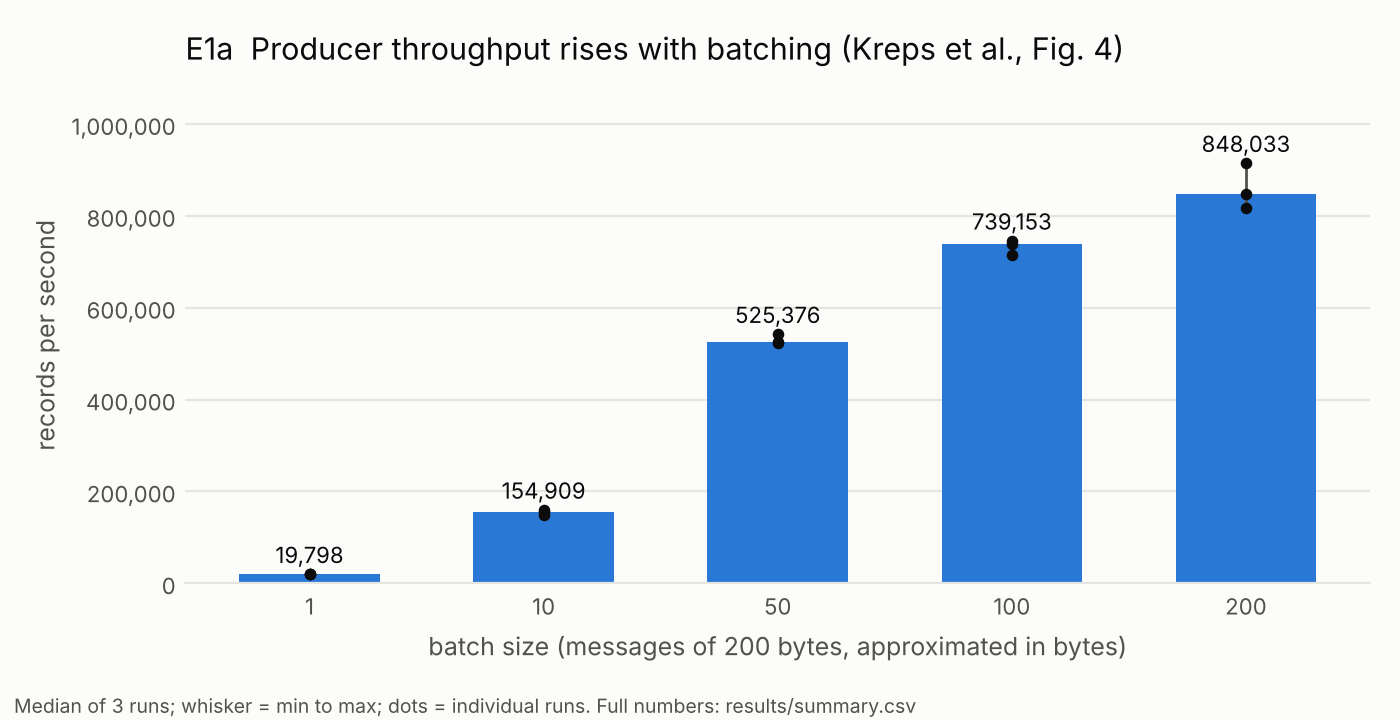
\includegraphics[width=0.8\textwidth]{e1a_producer_batching.png}
\caption{E1a: batching raises producer throughput.}
\label{fig:e1a}
\end{figure}

\subsection{E1b: continuous versus micro-batch (reproduction of Armbrust et al., Figure 7)}
A stateless pass-through job copies one topic to another. In continuous mode with 4 partitions, median
latency was 43 to 83 ms from 5,000 to 40,000 records per second (p99 0.3 to 0.9 s). At 80,000 records per
second its four tasks saturated: p50 rose to 1.8 s and p99 to 6.9 s. Micro-batch mode with a 100 ms
trigger kept up with the highest rate we could generate, at least 100,000 records per second, with
p50 between 0.27 and 0.62 s. See Figure~\ref{fig:e1b}.

\begin{figure}[H]
\centering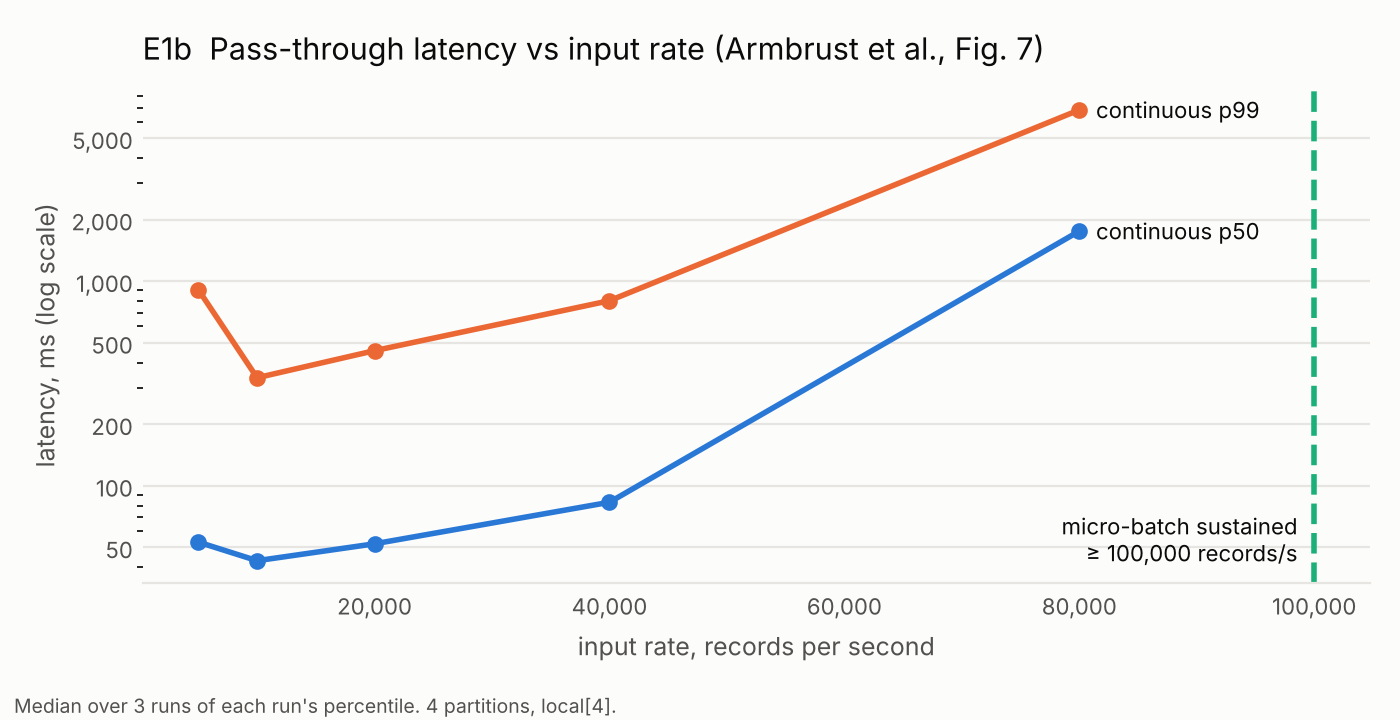
\includegraphics[width=0.85\textwidth]{e1b_continuous_vs_microbatch.png}
\caption{E1b: continuous mode has the lower latency until it saturates; micro-batch sustains a higher rate.}
\label{fig:e1b}
\end{figure}

\subsection{E1c: partitions and trigger interval (RQ1)}
Here we ran the real bars job in five-minute steps at 30,000, 60,000 and 90,000 records per second.
One partition sustained 75,000 records per second (one of three runs passed 90,000). Three and six
partitions, and every trigger from 500 ms to 5 s, sustained at least 90,000, which is the most our
generator could supply while sharing four cores with Spark. The 100 ms trigger reached its limit in one run of
three, at 75,000. Figure~\ref{fig:e1c-tp} shows this.

\begin{figure}[H]
\centering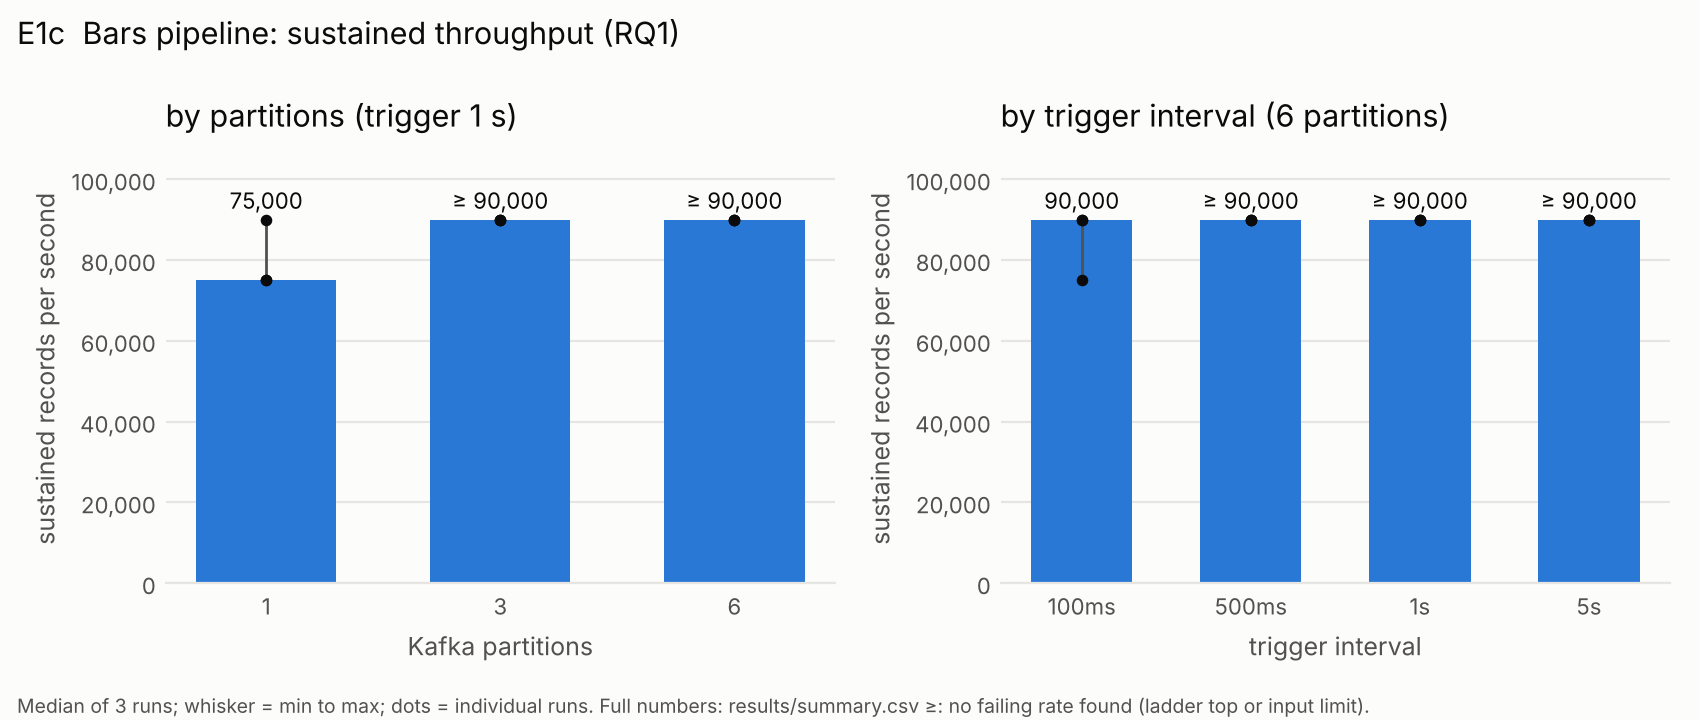
\includegraphics[width=0.85\textwidth]{e1c_sustained_throughput.png}
\caption{E1c: sustained throughput by partition count and trigger. Bars marked with a lower bound reached
our input limit before Spark's.}
\label{fig:e1c-tp}
\end{figure}

Bar latency runs from the window end plus the watermark to the moment the row is written.
Table~\ref{tab:e1c} gives the median p50.

\begin{table}[H]
\centering\small
\caption{E1c: bar latency p50 in seconds. The two sweeps ran on different CPUs (machine B, 2.30~GHz, and
machine A, 2.10~GHz), so we compare values only within one row.}
\label{tab:e1c}
\begin{tabular}{@{}lrr@{}}
\toprule
Setting & 30,000 records/s & 60,000 records/s \\
\midrule
1, 3, 6 partitions, trigger 1 s (machine B) & 2.5, 2.4, 2.5 & 2.4, 2.1, 3.5 \\
Trigger 100 ms, 500 ms, 1 s, 5 s, 6 partitions (machine A) & 2.2, \textbf{1.7}, 2.9, 7.2 & 6.4, 5.7, \textbf{4.9}, 8.7 \\
\bottomrule
\end{tabular}
\end{table}

The best trigger depends on the load. At 30,000 records per second a 500 ms trigger is fastest. At
60,000 a batch takes about two seconds whatever the trigger (batch duration p50 2.4 s at 100 ms, 2.1 s
at 500 ms, 2.0 s at 1 s), so a shorter trigger no longer starts batches sooner and only adds
per-batch overhead. There 1 s wins. A 5 s trigger always waits the longest. Below saturation the partition
count matters little, and at 60,000 six partitions on four cores cost more than three, because each
batch has more tasks and more state-store work. See Figures~\ref{fig:e1c-30} and~\ref{fig:e1c-60}.

\begin{figure}[H]
\centering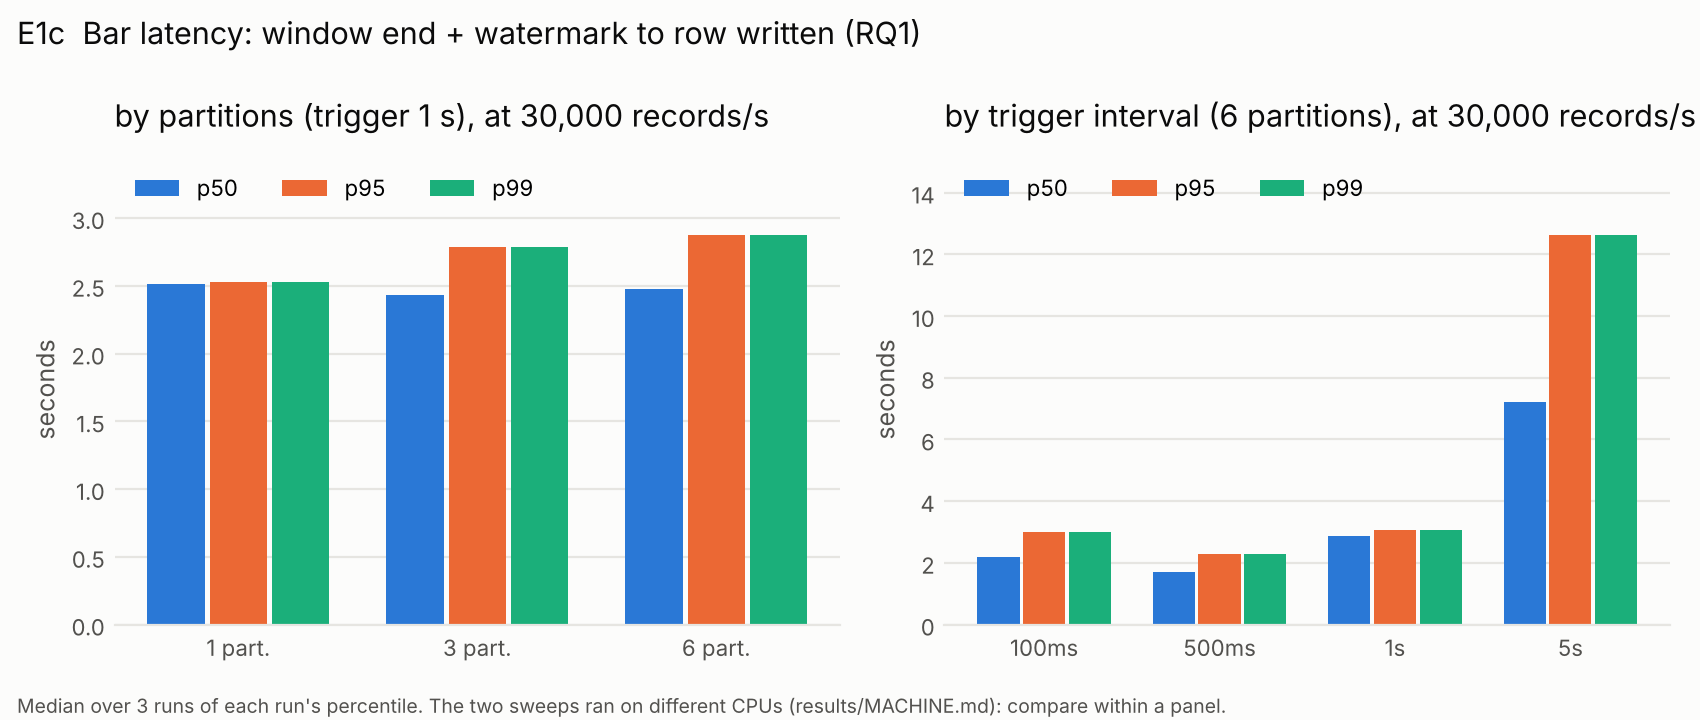
\includegraphics[width=0.85\textwidth]{e1c_bar_latency_30k.png}
\caption{E1c: bar latency at 30,000 records per second.}
\label{fig:e1c-30}
\end{figure}
\begin{figure}[H]
\centering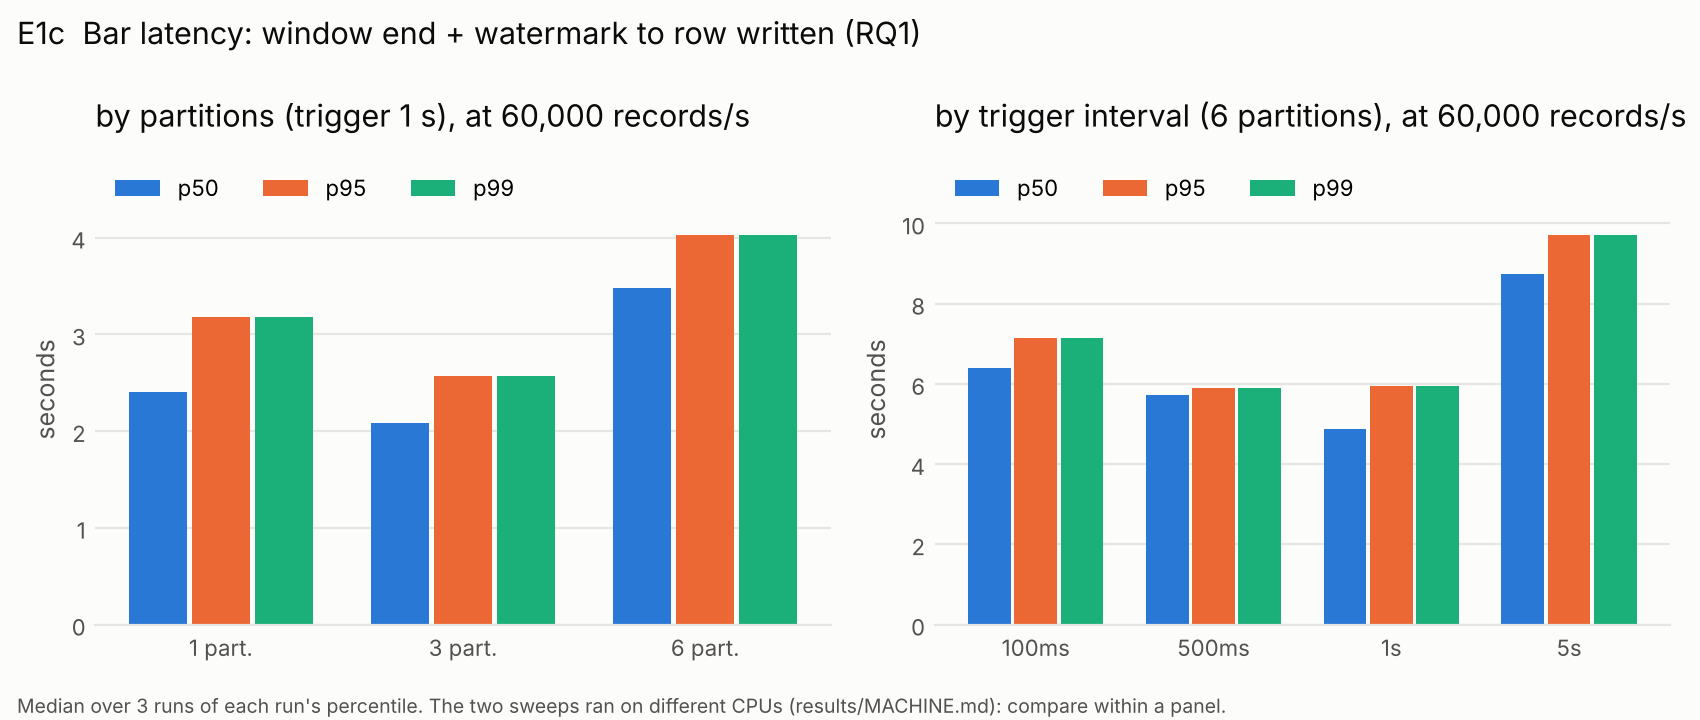
\includegraphics[width=0.85\textwidth]{e1c_bar_latency_60k.png}
\caption{E1c: bar latency at 60,000 records per second.}
\label{fig:e1c-60}
\end{figure}

\subsection{E2: broker crash (RQ2)}
We killed the broker that led partition 0 halfway through a 40-minute virtual run, with acks=1, with
acks=all, and with acks=all but no idempotence. No acknowledged trade was lost in any of the 12 kills.

With acks=all, writes stalled for 9.3 s [8.1 to 9.5] on every partition. The longest gap with no
acknowledgement anywhere was 9.1 s. The reason is that the dead broker stays in every partition's ISR
until the controller fences it, which takes the 9 s \code{broker.session.timeout.ms}. With acks=1 only the
partitions the dead broker led stalled, for 10.3 s [9.3 to 12.4], and the other partitions kept
acknowledging (longest gap anywhere 0.08 s). No duplicates appeared in these runs, even without
idempotence, although an earlier fault check did produce one (Section~\ref{sec:challenges}). A dry run
at a different rate did lose 2 acknowledged trades with acks=1, so loss is possible but rare.

One of the three runs without idempotence produced 33 wrong bars in a single minute even though Kafka
held every trade. The partitions resumed 3.8 s apart, the experiment's tenfold time compression turned
that into far more than the 10 s watermark, and Spark dropped those trades as late. This is a
real interaction between failover and watermarks, and we come back to it in Section~\ref{sec:limits}.
Figure~\ref{fig:e2} shows the stalls.

\begin{figure}[H]
\centering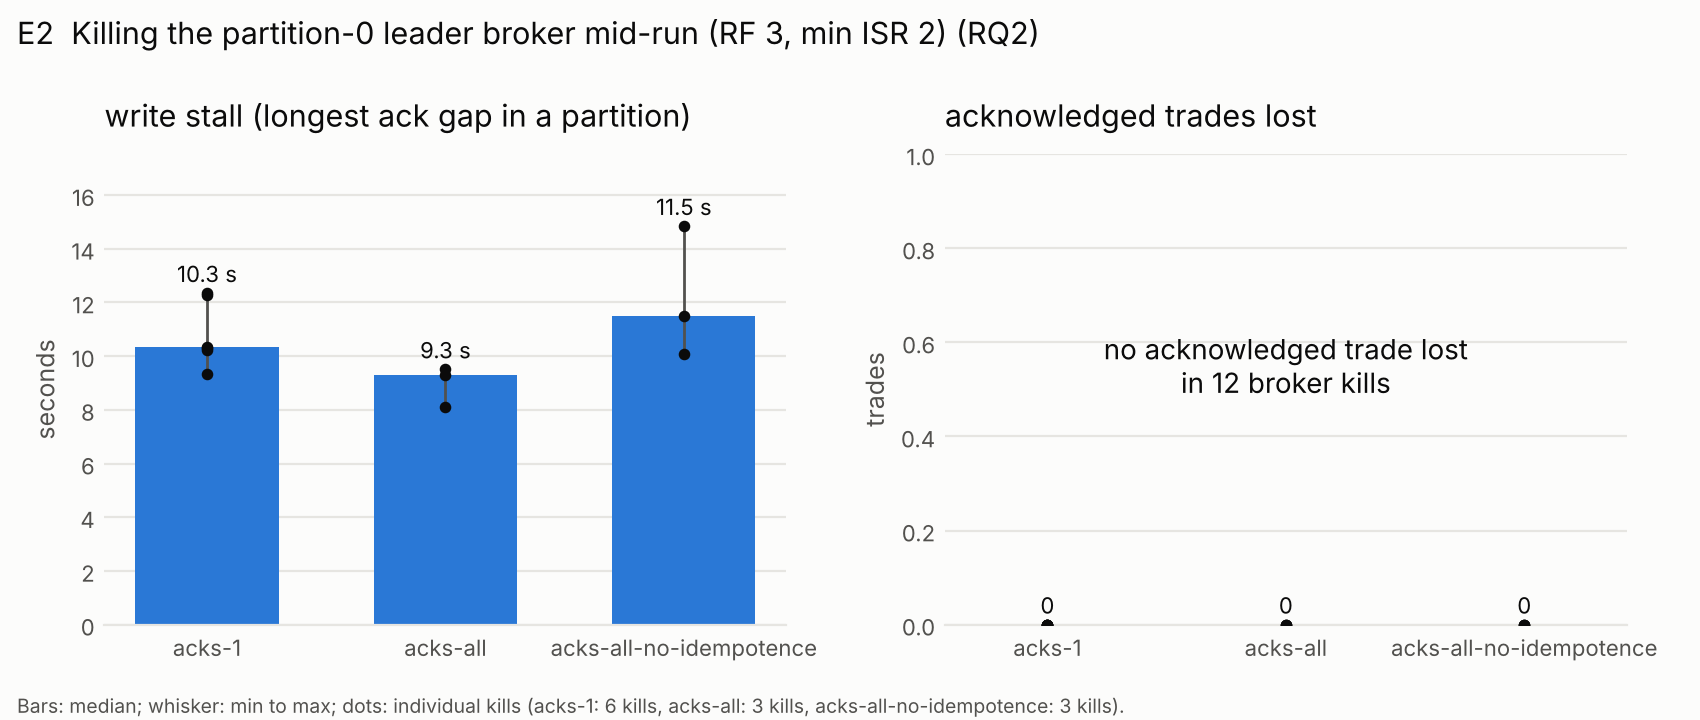
\includegraphics[width=0.9\textwidth]{e2_broker_crash.png}
\caption{E2: write stall and lost trades after a leader kill.}
\label{fig:e2}
\end{figure}

\subsection{E3: Spark crash (RQ2)}
We sent SIGKILL to the Spark container and restarted it at once on the same checkpoint. The first new bar
appeared 12.8 s [12.6 to 12.9] later in deterministic replay and 14.6 s [14.2 to 14.9] later on a live
stream, and the output was exact in all six runs. Almost all of that time is JVM and Spark start-up:
the first completed batch came 12.8 to 13.4 s after the restart. See Figure~\ref{fig:e3}.

\begin{figure}[H]
\centering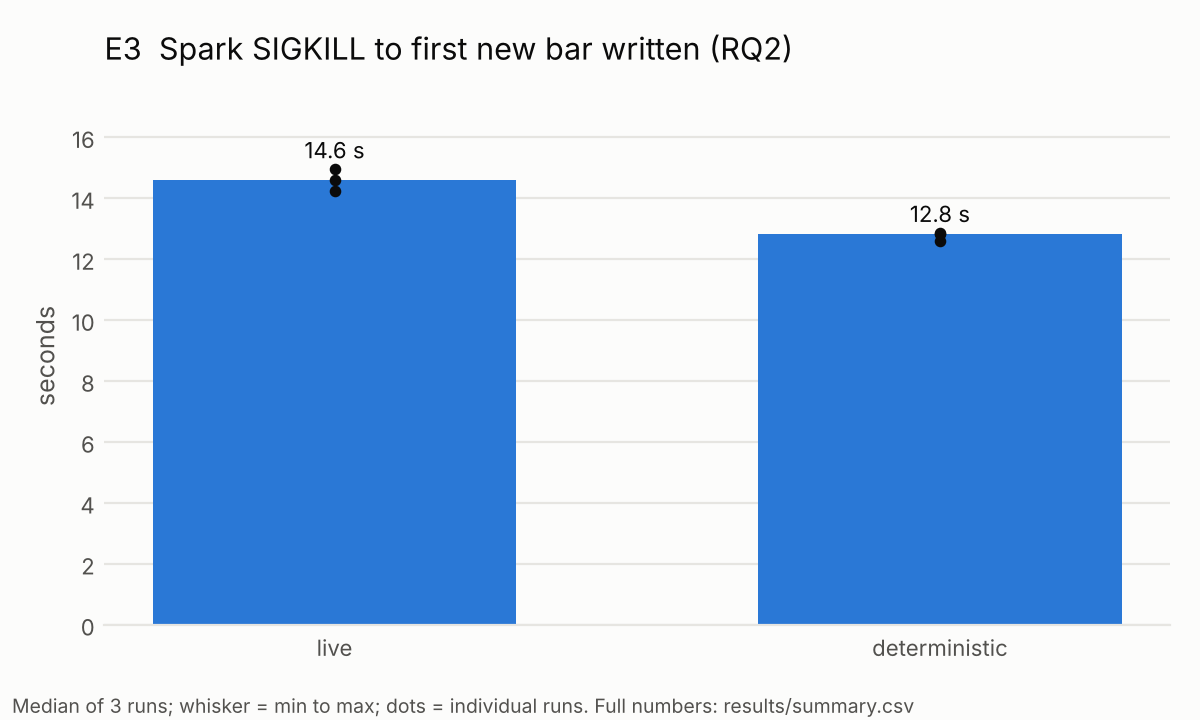
\includegraphics[width=0.7\textwidth]{e3_spark_recovery.png}
\caption{E3: time from the kill to the first new bar.}
\label{fig:e3}
\end{figure}

\subsection{E4: cost of exactly-once output (RQ3)}
We made Spark kill itself after the database commit and before Spark recorded the batch, so the restart
replays a batch that is already in the database. With plain inserts this left 300 duplicate bar rows in every
run, and with upserts none (three runs each). Without a crash, at 2,000 records per second, we could
not measure a cost for upserting. Batch duration p50 was 460 ms for inserts and 451 ms for upserts. Bar
latency p50 was 1.7 s [1.5 to 1.9] against 2.1 s [1.7 to 2.3], with overlapping ranges, and p99 was
2.45 s against 2.43 s. Both kept up. Figure~\ref{fig:e4} shows the results.

\begin{figure}[H]
\centering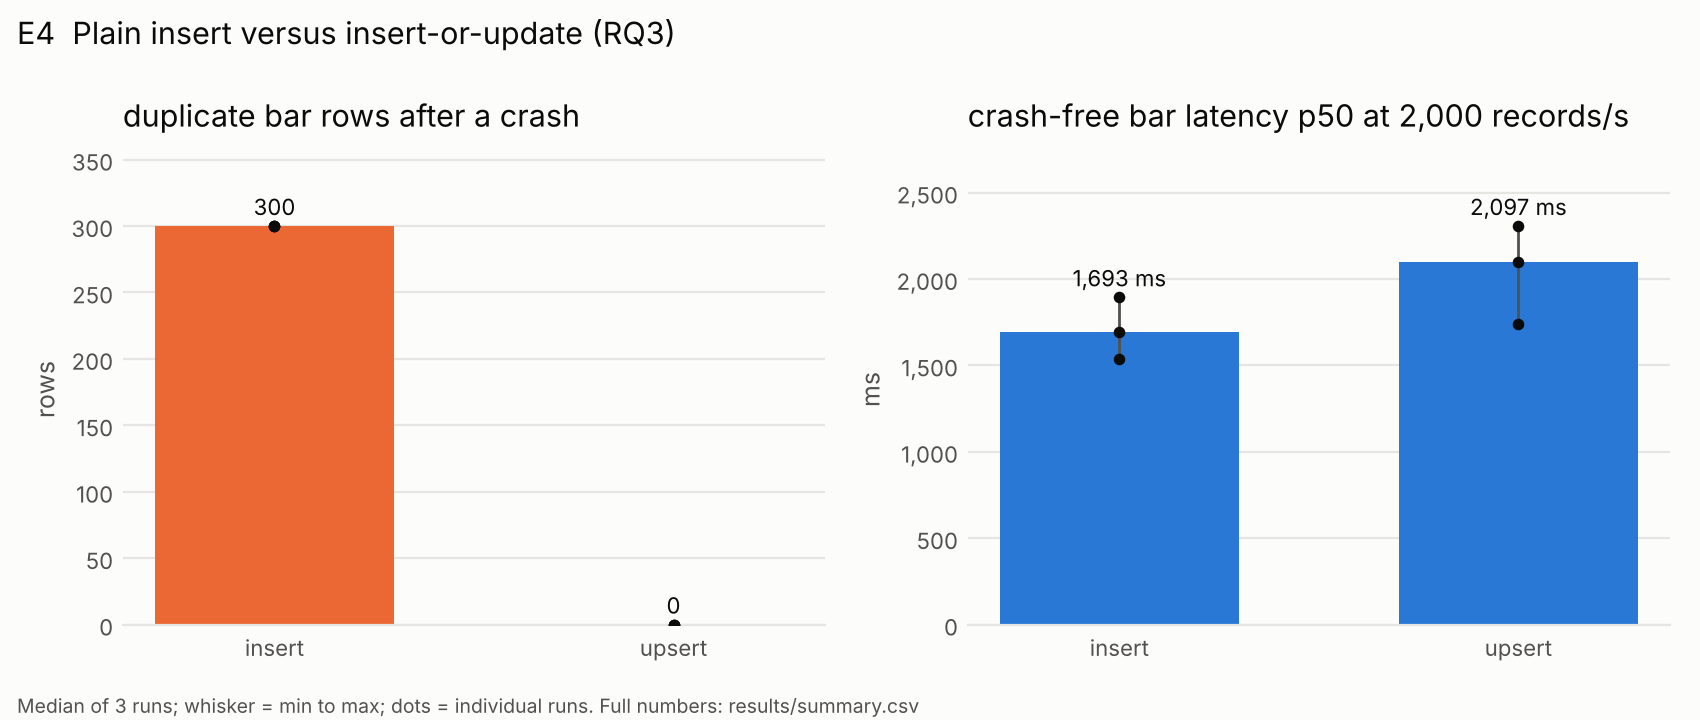
\includegraphics[width=0.9\textwidth]{e4_exactly_once.png}
\caption{E4: duplicate rows after a crash, and the cost of upserts without one.}
\label{fig:e4}
\end{figure}

\subsection{Live Coinbase run}
\label{sec:live}
We also ran the pipeline on live trades from Coinbase's public market-data feed for ten products (BTC, ETH,
SOL, XRP, DOGE, ADA, AVAX, LINK, LTC and BCH), on a Windows laptop with Docker Desktop, for more than 20
minutes. The producer connected to the feed, sent every trade to Kafka with acks=all, and saved a capture. The
dashboard filled with one-minute bars for all ten symbols, with Spark's lag at zero. No alert fired, which is
expected: live prices rarely move three standard deviations from their previous 30 one-minute returns, while the
synthetic data injects such shocks on purpose. After stopping the producer we ran the verifier against the
topic's own contents, because no generator file exists for live data. All 230 bars matched exactly (none
missing, extra, duplicated or different), and there were no alerts to match.

%------------------------------------------------------------------------------------------------
\section{Discussion: reproduction and extension}
\paragraph{Reproduction (a).} Batching raises producer throughput by more than an order of magnitude,
as Kreps et al.\ found, so the shape holds. Our unbatched rate is lower than theirs because every
one-record request is a round trip on a single shared four-core machine, and our batched rates are
higher because the producer and the CPU are newer. The paper used two dedicated 8-core machines, and we
approximate a batch of $n$ messages as $n \times 200$ bytes, since the Java producer sizes batches in bytes.

\paragraph{Reproduction (b).} Continuous processing gives much lower latency (tens of milliseconds
against hundreds) up to a saturation point, past which its latency climbs steeply, while micro-batch
sustains a higher input rate. The shape matches Armbrust et al. Their continuous latency was about
1 ms, and ours is tens of milliseconds because ours includes the producer's batching (\code{linger.ms}
of 5), a Kafka write with acks=all on three replicas, and the sink's own producer. The limit of one
core per partition on four cores is the constraint the paper describes, and we hit it.

\paragraph{Extension.} For RQ2, with replication factor 3 and a minimum ISR of 2, no acknowledged trade
was lost in 12 leader kills. The price of acks=all is a stall of about 9 s on every partition until the
dead broker is fenced. Acks=1 confines the stall to the dead broker's partitions but can lose
acknowledged writes, which we saw once, in a dry run. Spark recovers from its own crash in 13 to 15 s
with exact output. For RQ3, plain inserts are wrong after a crash (300 duplicate rows every time), and upserts
are exact at no cost we could measure at 2,000 records per second.

%------------------------------------------------------------------------------------------------
\section{Challenges}
\label{sec:challenges}
\begin{enumerate}
  \item \textbf{Determinism against late data.} An unpaced replay squeezes 40 virtual minutes into a few
        seconds, so a few milliseconds of skew between partitions looked like more than the 10 s watermark
        and trades would have been dropped as late. We now preload the topic before Spark starts.
  \item \textbf{Duplicates from producer retries.} With acks=all but idempotence off, killing a leader made
        the producer write one trade twice, and the verifier caught the wrong bar. Idempotence is now the
        default, and E2 measures the difference.
  \item \textbf{Measuring a write stall.} Looking at all partitions together hid the acks=1 behavior.
        We now compute the stall per partition from timestamped acknowledgements.
  \item \textbf{JVM warm-up} made the first latencies about twenty times worse, so we discard a warm-up
        period.
  \item \textbf{Continuous mode needs a core per partition.} With 6 partitions on 4 cores, two partitions were
        never processed, with no error. Continuous runs use 4 partitions.
  \item \textbf{Crashing between two commits.} A SIGKILL sent to PID 1 inside a container is ignored. The fault
        hook needed an init process and a kill of the driver JVM from inside \code{foreachBatch}.
  \item \textbf{Floating-point equality.} Fractional crypto sizes summed in a different order differ in
        the last bits, so the verifier allows a relative $10^{-9}$ for volume only.
  \item \textbf{Versions and tooling.} We checked that Kafka 4.4, Spark 4.2, PostgreSQL 18 and Grafana 13
        exist before pinning them, and had to build images behind a TLS-inspecting proxy and around Docker
        Hub rate limits.
  \item \textbf{Live data access.} The cloud development environment could not reach the Coinbase feed, so we
        first tested the adapter against a fake server that follows the protocol, and from captured sessions. We
        later ran it on a laptop (Section~\ref{sec:live}). Getting the stack to start on Windows took four fixes
        (a Linux-only default path, a missing image build, and two host ports that Windows had reserved or
        another project was using).
\end{enumerate}

%------------------------------------------------------------------------------------------------
\section{Reproducibility}
\label{sec:repro}
The repository holds everything needed to repeat the work. \code{docker compose up} starts the pipeline
and the demo. Image tags and Python packages are pinned and locked. A golden dataset with a SHA-256
manifest lets \code{make golden} replay a known stream through Kafka and Spark and check every bar and
alert against the oracle. \code{make bench-all} runs every experiment (about 12 hours), and
\code{uv run python -m bench.summarize} rebuilds every table and figure from the raw runs. Each run stores
its parameters, versions, git commit and machine. Continuous integration runs the linter, the unit tests and
the PostgreSQL integration tests on every push. The README explains how to run each step.

%------------------------------------------------------------------------------------------------
\section{Limitations: what one machine can and cannot show}
\label{sec:limits}
All three brokers, Spark (\code{local[4]}), PostgreSQL, Grafana, the generator and the measuring harness
ran on one virtual machine with 4 CPUs and 16 GB. Every container shares those four cores, one disk and
the loopback network. Our results are therefore sound for what they compare on this machine and weak as
absolute numbers.

\subsection{Throughput}
\begin{itemize}
  \item \textbf{Components compete for the same CPUs.} A measured rate is the pipeline's capacity while the
        generator, three brokers and PostgreSQL also run. On a cluster Kafka, Spark and the producers would
        have their own cores and every rate here would probably be higher. We report sustained rates as
        properties of this machine, not as limits of Kafka or Spark.
  \item \textbf{Our input is itself a ceiling.} The Python generator tops out near 100,000 records per second
        while Spark runs beside it. ``At least 90,000'' and ``micro-batch kept up at 100,000'' mean that the
        pipeline did not saturate before our input did. The true maximum is unknown.
  \item \textbf{Partition scaling is capped by cores.} More partitions than cores did not help (E1b, E1c). That
        shows the four-core limit and says nothing about how Kafka scales. The benefits of partitions in
        production, such as consumers on many machines and many disks, cannot appear here.
  \item \textbf{No network cost.} Replication between brokers crosses the loopback interface, so the latency of
        acks=all, which waits for replicas over a real network, is understated. E1a also differs from the
        paper because producer and broker share cores, where the paper used two 8-core machines.
  \item \textbf{One disk and the page cache.} Kafka depends on sequential disk writes and the page cache.
        Three brokers on one volume cannot show per-broker disk limits, and we did not enable \code{fsync}.
  \item \textbf{Changing hardware.} The virtual machine's CPU changed from 2.30 to 2.10 GHz between two
        experiments. We added a baseline setting (\code{p6-1s-b}) and compare triggers only within one machine
        state. Three runs per setting give a range, not a confidence interval.
  \item \textbf{Synthetic data.} Every measurement uses the seeded generator. Live Coinbase data appears only
        in the demonstration and in the short run of Section~\ref{sec:live}.
\end{itemize}

\subsection{Fault tolerance}
\begin{itemize}
  \item \textbf{A killed container is not a failed node.} \code{docker kill} stops one broker process at once.
        It does not model a network partition, a slow or full disk, a failed rack, a lost machine, or two
        brokers failing together. With three brokers on one host, the host is a single point of failure that
        none of our experiments can survive.
  \item \textbf{Detection time is configuration, not network behavior.} The 9 s stall in E2 equals the
        controller's \code{broker.session.timeout.ms} of 9,000 ms. On a real network, detection also depends on
        latency, partitions and clocks, and the stall could be shorter if tuned, or longer. We measured how this
        configuration reacts to a clean kill, not how fast Kafka recovers in general.
  \item \textbf{We injected the favorable failure.} A crashed leader's followers hold identical data, so a
        minimum ISR of 2 with unclean election off loses nothing. A leader that stays up but is cut off from
        its followers would test those settings harder, and we cannot produce that here.
  \item \textbf{Spark recovery excludes a cluster.} \code{local[4]} has no executors to lose, no rescheduling and
        no network shuffle. E3 measures checkpoint recovery of the driver (JVM start, state restore and
        replay), which is real, but not recovery on a standalone, YARN or Kubernetes cluster.
  \item \textbf{Time compression magnifies skew.} The crash experiments run virtual time ten times faster than
        the wall clock. A failover skew of a few seconds between partitions became tens of seconds of event
        time and made the 10 s watermark drop trades in one run (Section~\ref{sec:results}). With real-time data
        the same skew is ten times smaller relative to the watermark, so the failure would be rarer. The
        lesson that the watermark must exceed the partition skew still holds.
  \item \textbf{One local database.} A single PostgreSQL on the same machine has no network round trip and no
        competing writers, so the upsert cost we measured at 2,000 records per second is a lower bound for a
        remote or shared database.
\end{itemize}

\subsection{What still holds}
The correctness results do not depend on the machine. The bars and alerts match the oracle in every run,
no acknowledged trade was lost, and the duplicate rows in E4 follow from the protocol: a crash between
the database commit and Spark's commit replays the batch. The relative comparisons made on one machine
state (batching against none, continuous against micro-batch, trigger intervals, insert against upsert)
are valid for that machine, and their shapes agree with the published papers. We described Kafka's
security features (TLS, SASL, ACLs) but did not measure them. The harness could be pointed at a
multi-node cluster to extend the study.

%------------------------------------------------------------------------------------------------
\section{Conclusion}
\paragraph{RQ1.} The processing mode sets the latency floor. Continuous processing answers in tens of
milliseconds but saturates between 40,000 and 80,000 records per second on four cores, while micro-batch
trades hundreds of milliseconds for at least 100,000 records per second. For the bars pipeline the
trigger should match the load: 500 ms at moderate load, 1 s at high load, and 5 s was never best. More
partitions than cores did not help.

\paragraph{RQ2.} With replication factor 3 and a minimum ISR of 2, no acknowledged trade was lost in 12
leader kills. Acks=all stalls all writes for about 9 s until the dead broker is fenced, and acks=1 stalls
only its partitions but can lose acknowledged writes. A failover can also make Spark drop trades as late
when the watermark is shorter than the skew between partitions. Spark recovers from its own crash in
about 13 to 15 s with exact output.

\paragraph{RQ3.} Exactly-once output needs an idempotent sink. Plain inserts duplicated 300 rows after
every crash between the database commit and Spark's commit, upserts duplicated none, and at 2,000 records
per second the upsert cost nothing measurable.

\bibliographystyle{unsrt}
\bibliography{references}

%------------------------------------------------------------------------------------------------
\appendix
\section{Configuration of each experiment}
\label{app:config}
These tables come from \path{docker-compose.yml}, the topic script, the generator's defaults and the
experiment definitions in \path{bench/experiments/}. Each run also stores its own parameters in
\path{config.json} next to its raw output.

\subsection{Settings shared by all experiments}
\begin{table}[H]
\centering\small
\caption{Stack settings.}
\begin{tabularx}{\textwidth}{@{}>{\raggedright\arraybackslash}p{3.2cm}Y@{}}
\toprule
Component & Setting \\
\midrule
Kafka brokers & Image \code{apache/kafka:4.4.0}; 3 nodes, each broker and controller (KRaft combined mode); heap 1 GB per broker; \code{default.replication.factor=3}; \code{min.insync.replicas=2}; \code{unclean.leader.election.enable=false}; \code{auto.create.topics.enable=false}; PLAINTEXT listeners; no \code{log.flush.*} override; failure detection at the defaults (session timeout 9,000 ms, heartbeat 2,000 ms). \\
Topics & \code{trades}: 6 partitions by default (set per experiment), RF 3, min ISR 2, retention 1 day. \code{passthrough\_out}: same partitions as \code{trades}, RF 3, min ISR 2, \code{LogAppendTime}, retention 1 day. \code{perf\_test}: 1 partition, RF 1, min ISR 1, retention 1 hour. \\
Spark & Image \code{spark:4.2.1-scala2.13-java17-python3-ubuntu} with the Kafka connector \code{spark-sql-kafka-0-10\_2.13:4.2.1}; \code{--master local[4]}; driver memory 2 GB; container limit 4 CPUs and 3 GB; \code{spark.sql.shuffle.partitions=4}; session time zone UTC; \code{failOnDataLoss=true}; checkpoints on a named volume. \\
Bars job & Trigger 1 s; watermark 10 s; sink mode upsert; \code{startingOffsets=earliest}. \\
Pass-through job & Micro-batch trigger 100 ms, or continuous with a 1 s checkpoint interval; \code{startingOffsets=latest}. \\
PostgreSQL & Image \code{postgres:18.6}. \\
Producer (\code{confluent-kafka}) & \code{linger.ms=5}; \code{batch.size=1000000}; \code{retries=2147483647}; \code{queue.buffering.max.messages=500000}; \code{acks=all} with \code{enable.idempotence=true}, except where an experiment says otherwise (idempotence cannot be combined with acks=1). \\
\bottomrule
\end{tabularx}
\end{table}

\subsection{Settings per experiment}
\begin{table}[H]
\centering\footnotesize
\caption{Per-experiment settings. ``Records/s'' is the input rate.}
\begin{tabularx}{\textwidth}{@{}>{\raggedright\arraybackslash}p{1.1cm}YYY@{}}
\toprule
 & Kafka & Spark & Producer and input \\
\midrule
E1a & \code{perf\_test}: 1 partition, RF 1, min ISR 1; topic recreated for each setting & None & \code{kafka-producer-perf-test} inside \code{kafka-1}, 10 million records of 200 bytes, unlimited rate, \code{acks=0}; \code{batch.size} 0, 2,000, 10,000, 20,000, 40,000 bytes; \code{linger.ms} 0 (batch 1) or 10 \\
E1b & \code{trades} and \code{passthrough\_out}: 4 partitions, RF 3, min ISR 2 & Pass-through job; continuous (1 s checkpoint) or micro-batch (100 ms trigger); \code{startingOffsets=latest} & Realtime, \code{acks=all}, idempotent; continuous at 5,000, 10,000, 20,000, 40,000 and 80,000 records/s for 120 s (20 s warm-up); micro-batch at 40,000, 80,000 and 100,000 for 300 s (30 s warm-up) \\
E1c & \code{trades}: 1, 3 or 6 partitions, RF 3, min ISR 2; recreated before each step & Bars job, upsert sink; trigger 100 ms, 500 ms, 1 s or 5 s; \code{startingOffsets=latest} & Realtime, \code{acks=all}, idempotent, no closing trade; 30,000, 60,000 and 90,000 records/s, 300 s per step, 70 s warm-up; settings p1, p3, p6 with a 1 s trigger, and p6 with 100 ms, 500 ms, 5 s, plus a repeat of p6 at 1 s \\
E2 & \code{trades}: 6 partitions, RF 3, min ISR 2; the leader of partition 0 killed at 50\% of the run & Bars job, trigger 1 s, \code{startingOffsets=earliest} & Virtual mode, seed 42, 40 virtual minutes at 10 times speed, 1.0 trades per symbol per virtual second; acks=all with idempotence (3 kills), acks=1 (6 kills), acks=all without idempotence (3 kills) \\
E3 & \code{trades}: 6 partitions, RF 3, min ISR 2 & Bars job; SIGKILL at 50\% of the stream (live) or after batch 5 (deterministic, \code{maxOffsetsPerTrigger=5000}); restart at once on the same checkpoint & Live: virtual mode, seed 42, 40 minutes at 10 times speed. Deterministic: golden dataset (60,163 trades) preloaded and replayed at maximum speed. \code{acks=all}, idempotent \\
E4 & \code{trades}: 6 partitions, RF 3, min ISR 2 & Bars job; sink insert (\code{bars\_plain}) or upsert (\code{bars}); crash runs use \code{FAULT\_AFTER\_BATCH=5} and \code{maxOffsetsPerTrigger=5000} & Crash runs: golden replay. Cost runs: realtime at 2,000 records/s for 300 s, 70 s warm-up, no crash \\
\bottomrule
\end{tabularx}
\end{table}

\section{Machine and versions}
\label{app:machine}
Runs started on 11 November 2026 and finished on 12 November 2026 (72 runs, none failed). The development
virtual machine was moved between physical hosts when it restarted, so two CPUs appear. Both are 4-vCPU Intel
Xeon virtual machines with 15.7 GB of memory, Docker 29.9.2 and Linux 6.18.44: machine A at 2.10 GHz and
machine B at 2.30 GHz. Table~\ref{tab:machines} says which experiments ran where, and results are compared
only within one machine.

\begin{table}[H]
\centering\small
\caption{Where each experiment ran.}
\label{tab:machines}
\begin{tabular}{@{}ll@{}}
\toprule
Machine & Settings \\
\midrule
A (2.10 GHz) & E1c p6-100ms, p6-500ms, p6-5s and p6-1s-b; E2 (all); E3 (all); E4 crash runs \\
B (2.30 GHz) & E1a (all); E1b (all); E1c p1-1s, p3-1s and p6-1s; E4 cost runs \\
\bottomrule
\end{tabular}
\end{table}

\noindent Software: Apache Kafka 4.4.0, Apache Spark 4.2.1 (PySpark, Python 3.10 in the image), PostgreSQL
18.6, Grafana 13.3.0; on the host Python 3.13, confluent-kafka 2.16.1, psycopg 3.3.8, numpy 2.5.3 and
pandas 3.0.5, all pinned in the repository's lock file.
